\documentclass[8pt,aspectratio=169]{beamer}
\usetheme{Madrid}
\usepackage{graphicx,booktabs,adjustbox,multicol,amsmath,amssymb,listings,xcolor,colortbl}
\definecolor{mlblue}{RGB}{0,102,204}
\definecolor{mlpurple}{RGB}{51,51,178}
\definecolor{mllavender}{RGB}{173,173,224}
\definecolor{mllavender2}{RGB}{193,193,232}
\definecolor{mllavender3}{RGB}{204,204,235}
\definecolor{mllavender4}{RGB}{214,214,239}
\definecolor{mlorange}{RGB}{255,127,14}
\definecolor{mlgreen}{RGB}{44,160,44}
\definecolor{mlred}{RGB}{214,39,40}
\definecolor{mlgray}{RGB}{127,127,127}
% Solidity colors
\definecolor{solkeyword}{RGB}{0,102,153}
\definecolor{solstring}{RGB}{163,21,21}
\definecolor{solcomment}{RGB}{0,128,0}
\definecolor{solnumber}{RGB}{0,128,128}
\setbeamercolor{palette primary}{bg=mllavender3,fg=mlpurple}
\setbeamercolor{palette secondary}{bg=mllavender2,fg=mlpurple}
\setbeamercolor{palette tertiary}{bg=mllavender,fg=white}
\setbeamercolor{palette quaternary}{bg=mlpurple,fg=white}
\setbeamercolor{structure}{fg=mlpurple}
\setbeamercolor{title}{fg=mlpurple}
\setbeamercolor{frametitle}{fg=mlpurple,bg=mllavender3}
\setbeamercolor{block title}{bg=mllavender2,fg=mlpurple}
\setbeamercolor{block body}{bg=mllavender4,fg=black}
\setbeamertemplate{navigation symbols}{}
\setbeamertemplate{itemize items}[circle]
\setbeamersize{text margin left=5mm,text margin right=5mm}
\newcommand{\bottomnote}[1]{\vfill\vspace{-2mm}\textcolor{mllavender2}{\rule{\textwidth}{0.4pt}}\vspace{1mm}\footnotesize\textbf{#1}}
% Solidity language definition
\lstdefinelanguage{Solidity}{
  keywords={pragma, solidity, contract, function, public, private, external, internal, view, pure, payable, returns, return, if, else, for, while, mapping, address, uint, uint256, int, string, bool, bytes, bytes32, event, emit, modifier, require, constructor, memory, storage, calldata, msg, sender, value, this, new, delete, true, false, import, is, constant, override, virtual, interface, library, abstract, struct, enum, unchecked, assembly, abi, encode, decode, keccak256, receive, fallback},
  keywordstyle=\color{solkeyword}\bfseries,
  sensitive=true,
  comment=[l]{//},
  morecomment=[s]{/*}{*/},
  commentstyle=\color{solcomment}\ttfamily,
  stringstyle=\color{solstring}\ttfamily,
  morestring=[b]',
  morestring=[b]"
}
\lstset{language=Solidity,basicstyle=\ttfamily\scriptsize,breaklines=true,frame=single,backgroundcolor=\color{mllavender4},numbers=left,numberstyle=\tiny\color{mlgray},numbersep=5pt,tabsize=2,showstringspaces=false}
\usepackage{tikz,pgfplots}
\pgfplotsset{compat=1.18}
\usetikzlibrary{arrows.meta,positioning,shapes.geometric,calc,chains,decorations.pathmorphing,automata,fit}
\title{NFTs \& Digital Assets: A Quantitative Deep Dive}
\subtitle{Standalone Technical Lecture}
\author{Prof.~Dr.~Joerg Osterrieder}
\institute{University Lecture Series}
\date{\today}
\begin{document}

%% ============================================================
%% SECTION 0: OPENING
%% ============================================================

% Frame 1: Title
\begin{frame}
\titlepage
\end{frame}

% Frame 2: Lecture Roadmap
\begin{frame}{Lecture Roadmap}
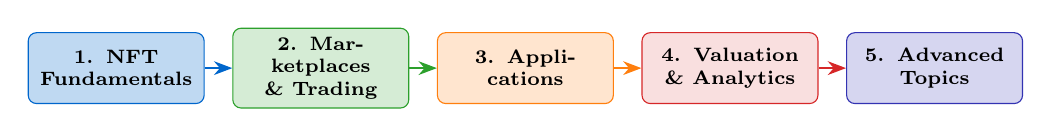
\begin{tikzpicture}[remember picture]
  \node[draw=mlblue, fill=mlblue!25, rounded corners=3pt, minimum width=2.1cm, minimum height=0.9cm, text width=2.0cm, align=center, font=\scriptsize\bfseries] (b1) {1. NFT\\Fundamentals};
  \node[draw=mlgreen, fill=mlgreen!20, rounded corners=3pt, minimum width=2.1cm, minimum height=0.9cm, text width=2.0cm, align=center, font=\scriptsize\bfseries, right=0.35cm of b1] (b2) {2. Marketplaces\\\& Trading};
  \node[draw=mlorange, fill=mlorange!20, rounded corners=3pt, minimum width=2.1cm, minimum height=0.9cm, text width=2.0cm, align=center, font=\scriptsize\bfseries, right=0.35cm of b2] (b3) {3. Applications};
  \node[draw=mlred, fill=mlred!15, rounded corners=3pt, minimum width=2.1cm, minimum height=0.9cm, text width=2.0cm, align=center, font=\scriptsize\bfseries, right=0.35cm of b3] (b4) {4. Valuation\\\& Analytics};
  \node[draw=mlpurple, fill=mlpurple!20, rounded corners=3pt, minimum width=2.1cm, minimum height=0.9cm, text width=2.0cm, align=center, font=\scriptsize\bfseries, right=0.35cm of b4] (b5) {5. Advanced\\Topics};
  \draw[-{Stealth}, thick, mlblue] (b1.east) -- (b2.west);
  \draw[-{Stealth}, thick, mlgreen] (b2.east) -- (b3.west);
  \draw[-{Stealth}, thick, mlorange] (b3.east) -- (b4.west);
  \draw[-{Stealth}, thick, mlred] (b4.east) -- (b5.west);
\end{tikzpicture}

\vspace{3mm}
\begin{columns}[T]
\column{0.5\textwidth}
\begin{block}{Learning Objectives}
\begin{itemize}\setlength{\itemsep}{1pt}
  \item Understand NFT mechanics and token standards
  \item Analyse marketplace dynamics and pricing
  \item Explore real-world NFT applications
  \item Apply quantitative valuation methods
  \item Evaluate advanced NFT architectures
\end{itemize}
\end{block}
\column{0.5\textwidth}
\begin{block}{Prerequisites}
\begin{itemize}\setlength{\itemsep}{1pt}
  \item Blockchain fundamentals (Lessons 1--2)
  \item Smart contract basics (Lessons 3--4)
  \item Ethereum architecture (Lesson 5)
  \item Basic programming knowledge
\end{itemize}
\end{block}
\end{columns}
\bottomnote{Duration: 90 minutes | 5 sections | \textasciitilde55 frames | Prerequisite: Lessons 1--5}
\end{frame}

% Frame 3: Table of Contents
\begin{frame}{Table of Contents}
\tableofcontents
\bottomnote{Navigate through 5 sections covering NFT fundamentals to advanced topics}
\end{frame}

%% ============================================================
%% SECTION 1: NFT FUNDAMENTALS & STANDARDS
%% ============================================================
\section{NFT Fundamentals \& Standards}

% Frame 4: Section Divider
\begin{frame}{Section 1: NFT Fundamentals \& Standards}
\begin{beamercolorbox}[sep=12pt,center,rounded=true,shadow=true]{palette quaternary}
  {\Large\bfseries Section 1: NFT Fundamentals \& Standards}\\[4pt]
  {\normalsize Building the conceptual and technical foundation for non-fungible tokens}
\end{beamercolorbox}

\vspace{4mm}
\begin{columns}[T]
\column{0.55\textwidth}
\begin{block}{What You Will Learn}
\begin{itemize}\setlength{\itemsep}{2pt}
  \item What makes a token non-fungible and why it matters
  \item The ERC-721 standard: interface, events, and patterns
  \item ERC-1155 multi-token standard and its advantages
  \item NFT metadata architecture and storage trade-offs
\end{itemize}
\end{block}
\column{0.42\textwidth}
\begin{block}{Frames in This Section}
\begin{itemize}\setlength{\itemsep}{1pt}
  \item Frame 4 --- Section overview
  \item Frame 5 --- What is an NFT?
  \item Frame 6 --- Fungible vs.\ Non-Fungible
  \item Frame 7 --- ERC-721 standard
  \item Frame 8 --- ERC-721 interface code
  \item Frame 9 --- ERC-1155 standard
  \item Frame 10 --- Metadata architecture
  \item Frame 11 --- Storage comparison
  \item Frame 12 --- Token ID \& ownership
  \item Frame 13 --- Minting process
  \item Frame 14 --- Section 1 summary
\end{itemize}
\end{block}
\end{columns}
\bottomnote{Section 1 | Frames 4--14 | NFT Fundamentals \& Standards}
\end{frame}

% Frame 5: What is a Non-Fungible Token?
\begin{frame}{What is a Non-Fungible Token?}
\begin{columns}[T]
\column{0.48\textwidth}
\begin{block}{Definition}
A \textbf{Non-Fungible Token (NFT)} is a cryptographic token on a blockchain that represents a \textit{unique} asset. Unlike fungible tokens, each NFT has a distinct identifier and is not interchangeable with any other token.
\end{block}
\vspace{2mm}
\begin{block}{Core Properties}
\begin{itemize}\setlength{\itemsep}{2pt}
  \item \textbf{Unique} --- each token has a distinct \texttt{tokenId}
  \item \textbf{Indivisible} --- cannot be split into fractions
  \item \textbf{Verifiable} --- ownership provable on-chain
  \item \textbf{Transferable} --- can be bought, sold, gifted
  \item \textbf{Programmable} --- smart contract logic attached
\end{itemize}
\end{block}

\column{0.48\textwidth}
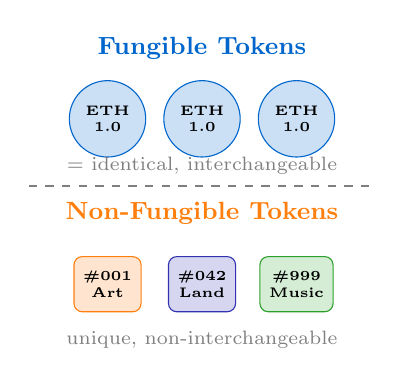
\begin{tikzpicture}[remember picture]
  % Fungible section
  \node[font=\small\bfseries, text=mlblue] (ftitle) at (2.2,4.2) {Fungible Tokens};
  \node[draw=mlblue, fill=mlblue!20, circle, minimum size=0.7cm, font=\tiny\bfseries, align=center] (fc1) at (1.0,3.3) {ETH\\1.0};
  \node[draw=mlblue, fill=mlblue!20, circle, minimum size=0.7cm, font=\tiny\bfseries, align=center] (fc2) at (2.2,3.3) {ETH\\1.0};
  \node[draw=mlblue, fill=mlblue!20, circle, minimum size=0.7cm, font=\tiny\bfseries, align=center] (fc3) at (3.4,3.3) {ETH\\1.0};
  \node[font=\scriptsize, text=mlgray] at (2.2,2.7) {= identical, interchangeable};

  % Non-Fungible section
  \node[font=\small\bfseries, text=mlorange] (nftitle) at (2.2,2.1) {Non-Fungible Tokens};
  \node[draw=mlorange, fill=mlorange!20, rounded corners=3pt, minimum size=0.7cm, font=\tiny\bfseries, align=center] (nfc1) at (1.0,1.2) {\#001\\Art};
  \node[draw=mlpurple, fill=mlpurple!20, rounded corners=3pt, minimum size=0.7cm, font=\tiny\bfseries, align=center] (nfc2) at (2.2,1.2) {\#042\\Land};
  \node[draw=mlgreen, fill=mlgreen!20, rounded corners=3pt, minimum size=0.7cm, font=\tiny\bfseries, align=center] (nfc3) at (3.4,1.2) {\#999\\Music};
  \node[font=\scriptsize, text=mlgray] at (2.2,0.5) {unique, non-interchangeable};

  % Divider
  \draw[dashed, mlgray, thick] (0,2.45) -- (4.4,2.45);
\end{tikzpicture}
\end{columns}
\bottomnote{Non-fungible means each token is unique and not interchangeable with any other token}
\end{frame}

% Frame 6: Fungible vs Non-Fungible: A Visual Comparison
\begin{frame}{Fungible vs Non-Fungible: A Visual Comparison}
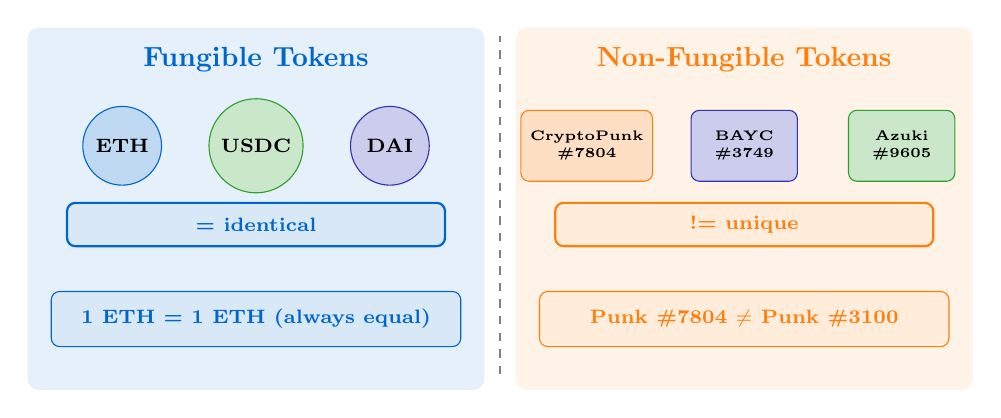
\begin{tikzpicture}[remember picture]
  % Background panels
  \fill[mlblue!10, rounded corners=4pt] (0,0) rectangle (5.8,4.6);
  \fill[mlorange!10, rounded corners=4pt] (6.2,0) rectangle (12.0,4.6);

  % Headers
  \node[font=\normalsize\bfseries, text=mlblue] at (2.9,4.2) {Fungible Tokens};
  \node[font=\normalsize\bfseries, text=mlorange] at (9.1,4.2) {Non-Fungible Tokens};

  % Fungible examples
  \node[draw=mlblue, fill=mlblue!25, circle, minimum size=1.0cm, font=\scriptsize\bfseries, align=center] at (1.2,3.1) {ETH};
  \node[draw=mlgreen, fill=mlgreen!25, circle, minimum size=1.0cm, font=\scriptsize\bfseries, align=center] at (2.9,3.1) {USDC};
  \node[draw=mlpurple, fill=mlpurple!25, circle, minimum size=1.0cm, font=\scriptsize\bfseries, align=center] at (4.6,3.1) {DAI};

  \node[draw=mlblue, thick, rounded corners=3pt, fill=mlblue!15, minimum width=4.8cm, minimum height=0.55cm, font=\scriptsize\bfseries, align=center, text=mlblue] at (2.9,2.1) {= identical};

  % Non-fungible examples
  \node[draw=mlorange, fill=mlorange!25, rounded corners=3pt, minimum width=1.35cm, minimum height=0.9cm, font=\tiny\bfseries, align=center] at (7.1,3.1) {CryptoPunk\\\#7804};
  \node[draw=mlpurple, fill=mlpurple!25, rounded corners=3pt, minimum width=1.35cm, minimum height=0.9cm, font=\tiny\bfseries, align=center] at (9.1,3.1) {BAYC\\\#3749};
  \node[draw=mlgreen, fill=mlgreen!25, rounded corners=3pt, minimum width=1.35cm, minimum height=0.9cm, font=\tiny\bfseries, align=center] at (11.1,3.1) {Azuki\\\#9605};

  \node[draw=mlorange, thick, rounded corners=3pt, fill=mlorange!15, minimum width=4.8cm, minimum height=0.55cm, font=\scriptsize\bfseries, align=center, text=mlorange] at (9.1,2.1) {!= unique};

  % Bottom comparison
  \node[draw=mlblue, fill=mlblue!15, rounded corners=3pt, minimum width=5.2cm, minimum height=0.7cm, font=\scriptsize\bfseries, align=center, text=mlblue] at (2.9,0.9) {1 ETH = 1 ETH (always equal)};
  \node[draw=mlorange, fill=mlorange!15, rounded corners=3pt, minimum width=5.2cm, minimum height=0.7cm, font=\scriptsize\bfseries, align=center, text=mlorange] at (9.1,0.9) {Punk \#7804 $\neq$ Punk \#3100};

  % Divider line
  \draw[thick, mlgray, dashed] (6.0,0.2) -- (6.0,4.5);
\end{tikzpicture}
\bottomnote{Fungibility is about substitutability -- fungible tokens are interchangeable, NFTs are not}
\end{frame}

% Frame 7: ERC-721: The NFT Standard
\begin{frame}{ERC-721: The NFT Standard}
\begin{columns}[T]
\column{0.50\textwidth}
\begin{block}{Core Interface Functions}
\begin{itemize}\setlength{\itemsep}{2pt}
  \item \texttt{balanceOf(owner)} --- count NFTs owned
  \item \texttt{ownerOf(tokenId)} --- get current owner
  \item \texttt{transferFrom(from, to, id)} --- transfer token
  \item \texttt{approve(to, tokenId)} --- allow one transfer
  \item \texttt{safeTransferFrom(...)} --- transfer with safety check
  \item \texttt{tokenURI(tokenId)} --- get metadata URI
\end{itemize}
\end{block}
\vspace{2mm}
\begin{block}{Key Events}
\begin{itemize}\setlength{\itemsep}{2pt}
  \item \texttt{Transfer(from, to, tokenId)} --- ownership change
  \item \texttt{Approval(owner, approved, tokenId)} --- approval set
\end{itemize}
\end{block}

\column{0.46\textwidth}
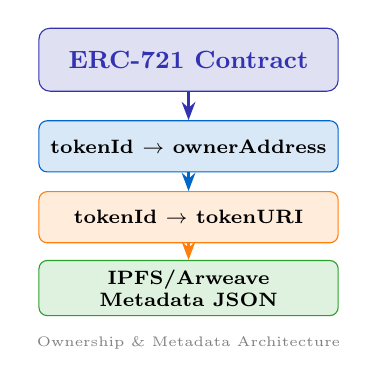
\begin{tikzpicture}[remember picture]
  % Contract box
  \node[draw=mlpurple, fill=mlpurple!15, rounded corners=4pt, minimum width=3.8cm, minimum height=0.8cm, font=\small\bfseries, align=center, text=mlpurple] (contract) at (1.9,4.0) {ERC-721 Contract};

  % Mapping box
  \node[draw=mlblue, fill=mlblue!15, rounded corners=3pt, minimum width=3.8cm, minimum height=0.65cm, font=\scriptsize\bfseries, align=center] (mapping) at (1.9,2.9) {tokenId $\to$ ownerAddress};

  % TokenURI box
  \node[draw=mlorange, fill=mlorange!15, rounded corners=3pt, minimum width=3.8cm, minimum height=0.65cm, font=\scriptsize\bfseries, align=center] (uri) at (1.9,2.0) {tokenId $\to$ tokenURI};

  % Metadata box
  \node[draw=mlgreen, fill=mlgreen!15, rounded corners=3pt, minimum width=3.8cm, minimum height=0.65cm, font=\scriptsize\bfseries, align=center] (meta) at (1.9,1.1) {IPFS/Arweave\\Metadata JSON};

  % Arrows
  \draw[-{Stealth}, thick, mlpurple] (contract.south) -- (mapping.north);
  \draw[-{Stealth}, thick, mlblue] (mapping.south) -- (uri.north);
  \draw[-{Stealth}, thick, mlorange] (uri.south) -- (meta.north);

  % Label
  \node[font=\tiny, text=mlgray, align=center] at (1.9,0.4) {Ownership \& Metadata Architecture};
\end{tikzpicture}
\end{columns}
\bottomnote{ERC-721 was proposed in January 2018 (EIP-721) and is the foundation for most NFT projects}
\end{frame}

% Frame 8: ERC-721 Interface [FRAGILE]
\begin{frame}[fragile]{ERC-721 Interface}
\begin{columns}[T]
\column{0.40\textwidth}
\begin{block}{Key Functions Explained}
\begin{itemize}\setlength{\itemsep}{2pt}
  \item \texttt{balanceOf} --- returns total NFTs held by an address
  \item \texttt{ownerOf} --- resolves tokenId to owner address
  \item \texttt{transferFrom} --- moves token between addresses
  \item \texttt{approve} --- delegates transfer right for one token
  \item \texttt{tokenURI} --- returns off-chain metadata location
\end{itemize}
\end{block}
\vspace{2mm}
\begin{block}{Implementation Note}
All transfers must emit the \texttt{Transfer} event. Safe transfers check if the receiver implements \texttt{IERC721Receiver}.
\end{block}

\column{0.57\textwidth}
\begin{lstlisting}[language=Solidity]
// SPDX-License-Identifier: MIT
pragma solidity ^0.8.0;

interface IERC721 {
    function balanceOf(address owner)
        external view returns (uint256);
    function ownerOf(uint256 tokenId)
        external view returns (address);
    function transferFrom(
        address from, address to,
        uint256 tokenId
    ) external;
    function approve(
        address to, uint256 tokenId
    ) external;
    function tokenURI(uint256 tokenId)
        external view returns (string memory);
}
\end{lstlisting}
\end{columns}
\bottomnote{The ERC-721 interface defines the minimal functions every NFT contract must implement}
\end{frame}

% Frame 9: ERC-1155: The Multi-Token Standard
\begin{frame}{ERC-1155: The Multi-Token Standard}
\begin{columns}[T]
\column{0.48\textwidth}
\begin{block}{ERC-1155 Advantages}
\begin{itemize}\setlength{\itemsep}{2pt}
  \item \textbf{Batch transfers} --- move many tokens in one call
  \item \textbf{Gas efficiency} --- up to 90\% savings vs ERC-721
  \item \textbf{Mixed types} --- fungible and non-fungible together
  \item \textbf{Single contract} --- manages entire token ecosystem
  \item \textbf{Atomic swaps} --- safe multi-token exchanges
\end{itemize}
\end{block}
\vspace{2mm}
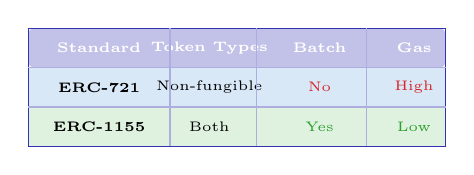
\begin{tikzpicture}[remember picture]
  % Comparison table header
  \fill[mlpurple!30, rounded corners=2pt] (0,1.85) rectangle (5.3,2.35);
  \node[font=\tiny\bfseries, text=white] at (0.9,2.1) {Standard};
  \node[font=\tiny\bfseries, text=white] at (2.3,2.1) {Token Types};
  \node[font=\tiny\bfseries, text=white] at (3.7,2.1) {Batch};
  \node[font=\tiny\bfseries, text=white] at (4.9,2.1) {Gas};
  % Row 1
  \fill[mlblue!15] (0,1.35) rectangle (5.3,1.85);
  \node[font=\tiny\bfseries] at (0.9,1.6) {ERC-721};
  \node[font=\tiny] at (2.3,1.6) {Non-fungible};
  \node[font=\tiny, text=mlred] at (3.7,1.6) {No};
  \node[font=\tiny, text=mlred] at (4.9,1.6) {High};
  % Row 2
  \fill[mlgreen!15] (0,0.85) rectangle (5.3,1.35);
  \node[font=\tiny\bfseries] at (0.9,1.1) {ERC-1155};
  \node[font=\tiny] at (2.3,1.1) {Both};
  \node[font=\tiny, text=mlgreen] at (3.7,1.1) {Yes};
  \node[font=\tiny, text=mlgreen] at (4.9,1.1) {Low};
  % Border
  \draw[mlpurple, thin] (0,0.85) rectangle (5.3,2.35);
  \draw[mlpurple!40, thin] (1.8,0.85) -- (1.8,2.35);
  \draw[mlpurple!40, thin] (2.9,0.85) -- (2.9,2.35);
  \draw[mlpurple!40, thin] (4.3,0.85) -- (4.3,2.35);
  \draw[mlpurple!40, thin] (0,1.35) -- (5.3,1.35);
  \draw[mlpurple!40, thin] (0,1.85) -- (5.3,1.85);
\end{tikzpicture}

\column{0.48\textwidth}
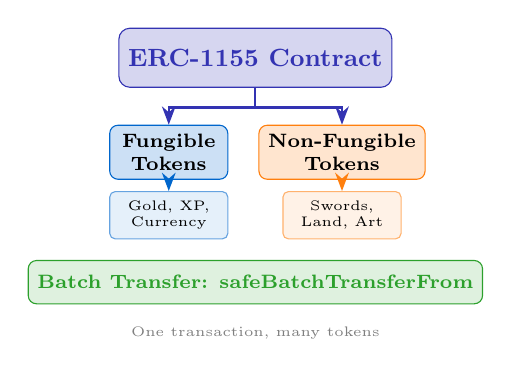
\begin{tikzpicture}[remember picture]
  % Single contract node
  \node[draw=mlpurple, fill=mlpurple!20, rounded corners=4pt, minimum width=3.4cm, minimum height=0.75cm, font=\small\bfseries, align=center, text=mlpurple] (sc) at (1.7,4.2) {ERC-1155 Contract};

  % Fungible branch
  \node[draw=mlblue, fill=mlblue!20, rounded corners=3pt, minimum width=1.5cm, minimum height=0.65cm, font=\scriptsize\bfseries, align=center] (ft) at (0.6,3.0) {Fungible\\Tokens};
  \node[draw=mlblue!60, fill=mlblue!10, rounded corners=2pt, minimum width=1.5cm, minimum height=0.5cm, font=\tiny, align=center] (fe) at (0.6,2.2) {Gold, XP,\\Currency};

  % Non-fungible branch
  \node[draw=mlorange, fill=mlorange!20, rounded corners=3pt, minimum width=1.5cm, minimum height=0.65cm, font=\scriptsize\bfseries, align=center] (nft) at (2.8,3.0) {Non-Fungible\\Tokens};
  \node[draw=mlorange!60, fill=mlorange!10, rounded corners=2pt, minimum width=1.5cm, minimum height=0.5cm, font=\tiny, align=center] (nfe) at (2.8,2.2) {Swords,\\Land, Art};

  \draw[-{Stealth}, thick, mlpurple] (sc.south) -- ++(0,-0.25) -| (ft.north);
  \draw[-{Stealth}, thick, mlpurple] (sc.south) -- ++(0,-0.25) -| (nft.north);
  \draw[-{Stealth}, thick, mlblue] (ft.south) -- (fe.north);
  \draw[-{Stealth}, thick, mlorange] (nft.south) -- (nfe.north);

  % Batch transfer label
  \node[draw=mlgreen, fill=mlgreen!15, rounded corners=3pt, minimum width=3.4cm, minimum height=0.55cm, font=\scriptsize\bfseries, align=center, text=mlgreen] at (1.7,1.35) {Batch Transfer: safeBatchTransferFrom};
  \node[font=\tiny, text=mlgray, align=center] at (1.7,0.7) {One transaction, many tokens};
\end{tikzpicture}
\end{columns}
\bottomnote{ERC-1155 supports both fungible and non-fungible tokens in a single contract, reducing gas costs}
\end{frame}

% Frame 10: NFT Metadata Architecture
\begin{frame}{NFT Metadata Architecture}
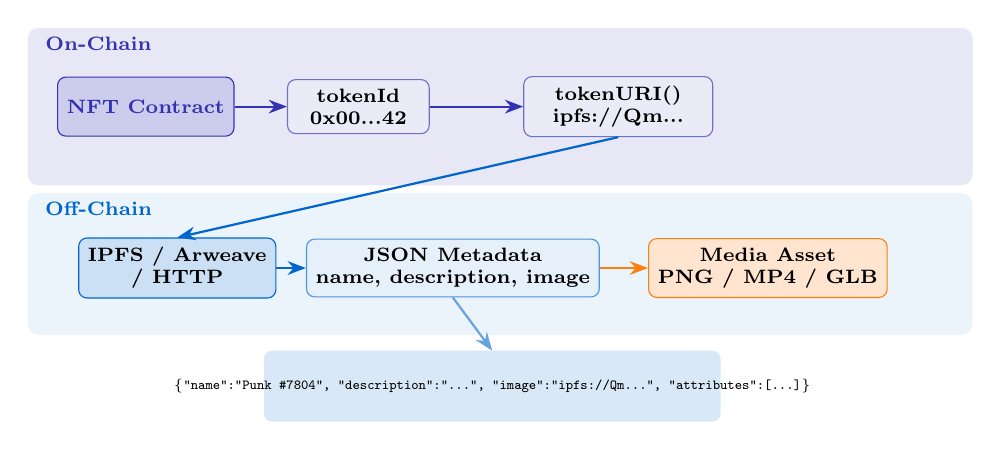
\begin{tikzpicture}[remember picture]
  %--- On-chain layer ---
  \fill[mlpurple!12, rounded corners=4pt] (0.0,3.0) rectangle (12.0,5.0);
  \node[font=\scriptsize\bfseries, text=mlpurple] at (0.9,4.8) {On-Chain};

  \node[draw=mlpurple, fill=mlpurple!25, rounded corners=3pt, minimum width=2.2cm, minimum height=0.75cm, font=\scriptsize\bfseries, align=center, text=mlpurple] (contract) at (1.5,4.0) {NFT Contract};
  \node[draw=mlpurple!70, fill=mlpurple!10, rounded corners=3pt, minimum width=1.8cm, minimum height=0.65cm, font=\scriptsize\bfseries, align=center] (tokenid) at (4.2,4.0) {tokenId\\0x00...42};
  \node[draw=mlpurple!70, fill=mlpurple!10, rounded corners=3pt, minimum width=2.4cm, minimum height=0.65cm, font=\scriptsize\bfseries, align=center] (tokuri) at (7.5,4.0) {tokenURI()\\ipfs://Qm...};

  \draw[-{Stealth}, thick, mlpurple] (contract.east) -- (tokenid.west);
  \draw[-{Stealth}, thick, mlpurple] (tokenid.east) -- (tokuri.west);

  %--- Off-chain layer ---
  \fill[mlblue!8, rounded corners=4pt] (0.0,1.1) rectangle (12.0,2.9);
  \node[font=\scriptsize\bfseries, text=mlblue] at (0.9,2.7) {Off-Chain};

  \node[draw=mlblue, fill=mlblue!20, rounded corners=3pt, minimum width=2.2cm, minimum height=0.65cm, font=\scriptsize\bfseries, align=center] (ipfs) at (1.9,1.95) {IPFS / Arweave\\/ HTTP};
  \node[draw=mlblue!70, fill=mlblue!10, rounded corners=3pt, minimum width=3.0cm, minimum height=0.65cm, font=\scriptsize\bfseries, align=center] (json) at (5.4,1.95) {JSON Metadata\\name, description, image};
  \node[draw=mlorange, fill=mlorange!20, rounded corners=3pt, minimum width=2.4cm, minimum height=0.65cm, font=\scriptsize\bfseries, align=center] (media) at (9.4,1.95) {Media Asset\\PNG / MP4 / GLB};

  \draw[-{Stealth}, thick, mlblue] (tokuri.south) -- (ipfs.north);
  \draw[-{Stealth}, thick, mlblue] (ipfs.east) -- (json.west);
  \draw[-{Stealth}, thick, mlorange] (json.east) -- (media.west);

  %--- JSON structure box ---
  \fill[mlblue!15, rounded corners=3pt] (3.0,0.0) rectangle (8.8,0.9);
  \node[font=\tiny\ttfamily, align=left] at (5.9,0.45)
    {\{"name":"Punk \#7804", "description":"...", "image":"ipfs://Qm...", "attributes":[...]\}};

  \draw[-{Stealth}, thick, mlblue!60] (json.south) -- (5.9,0.9);
\end{tikzpicture}
\bottomnote{NFT metadata follows the ERC-721 Metadata JSON Schema -- name, description, image, and attributes}
\end{frame}

% Frame 11: On-Chain vs Off-Chain Storage
\begin{frame}{On-Chain vs Off-Chain Storage}
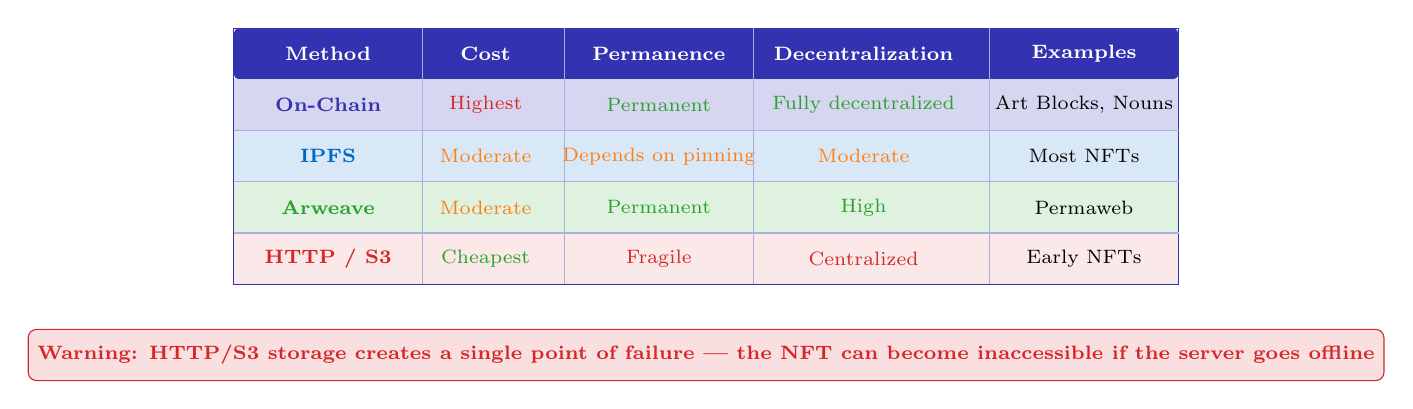
\begin{tikzpicture}[remember picture]
  % Header row
  \fill[mlpurple, rounded corners=2pt] (0,5.1) rectangle (12.0,5.75);
  \node[font=\scriptsize\bfseries, text=white, align=center] at (1.2,5.425) {Method};
  \node[font=\scriptsize\bfseries, text=white, align=center] at (3.2,5.425) {Cost};
  \node[font=\scriptsize\bfseries, text=white, align=center] at (5.4,5.425) {Permanence};
  \node[font=\scriptsize\bfseries, text=white, align=center] at (8.0,5.425) {Decentralization};
  \node[font=\scriptsize\bfseries, text=white, align=center] at (10.8,5.425) {Examples};

  % Row 1: On-chain
  \fill[mlpurple!20] (0,4.45) rectangle (12.0,5.1);
  \node[font=\scriptsize\bfseries, text=mlpurple, align=center] at (1.2,4.775) {On-Chain};
  \node[font=\scriptsize, text=mlred, align=center] at (3.2,4.775) {Highest};
  \node[font=\scriptsize, text=mlgreen, align=center] at (5.4,4.775) {Permanent};
  \node[font=\scriptsize, text=mlgreen, align=center] at (8.0,4.775) {Fully decentralized};
  \node[font=\scriptsize, align=center] at (10.8,4.775) {Art Blocks, Nouns};

  % Row 2: IPFS
  \fill[mlblue!15] (0,3.8) rectangle (12.0,4.45);
  \node[font=\scriptsize\bfseries, text=mlblue, align=center] at (1.2,4.125) {IPFS};
  \node[font=\scriptsize, text=mlorange, align=center] at (3.2,4.125) {Moderate};
  \node[font=\scriptsize, text=mlorange, align=center] at (5.4,4.125) {Depends on pinning};
  \node[font=\scriptsize, text=mlorange, align=center] at (8.0,4.125) {Moderate};
  \node[font=\scriptsize, align=center] at (10.8,4.125) {Most NFTs};

  % Row 3: Arweave
  \fill[mlgreen!15] (0,3.15) rectangle (12.0,3.8);
  \node[font=\scriptsize\bfseries, text=mlgreen, align=center] at (1.2,3.475) {Arweave};
  \node[font=\scriptsize, text=mlorange, align=center] at (3.2,3.475) {Moderate};
  \node[font=\scriptsize, text=mlgreen, align=center] at (5.4,3.475) {Permanent};
  \node[font=\scriptsize, text=mlgreen, align=center] at (8.0,3.475) {High};
  \node[font=\scriptsize, align=center] at (10.8,3.475) {Permaweb};

  % Row 4: HTTP/S3
  \fill[mlred!10] (0,2.5) rectangle (12.0,3.15);
  \node[font=\scriptsize\bfseries, text=mlred, align=center] at (1.2,2.825) {HTTP / S3};
  \node[font=\scriptsize, text=mlgreen, align=center] at (3.2,2.825) {Cheapest};
  \node[font=\scriptsize, text=mlred, align=center] at (5.4,2.825) {Fragile};
  \node[font=\scriptsize, text=mlred, align=center] at (8.0,2.825) {Centralized};
  \node[font=\scriptsize, align=center] at (10.8,2.825) {Early NFTs};

  % Table border and column lines
  \draw[mlpurple, thin] (0,2.5) rectangle (12.0,5.75);
  \draw[mlpurple!40, thin] (2.4,2.5) -- (2.4,5.75);
  \draw[mlpurple!40, thin] (4.2,2.5) -- (4.2,5.75);
  \draw[mlpurple!40, thin] (6.6,2.5) -- (6.6,5.75);
  \draw[mlpurple!40, thin] (9.6,2.5) -- (9.6,5.75);
  \draw[mlpurple!40, thin] (0,3.15) -- (12.0,3.15);
  \draw[mlpurple!40, thin] (0,3.8) -- (12.0,3.8);
  \draw[mlpurple!40, thin] (0,4.45) -- (12.0,4.45);

  % Warning box
  \node[draw=mlred, fill=mlred!15, rounded corners=3pt, minimum width=11.6cm, minimum height=0.65cm, font=\scriptsize\bfseries, align=center, text=mlred] at (6.0,1.6) {Warning: HTTP/S3 storage creates a single point of failure --- the NFT can become inaccessible if the server goes offline};
\end{tikzpicture}
\bottomnote{Storage choice is the most critical design decision for NFT longevity}
\end{frame}

% Frame 12: Token ID and Ownership Mapping
\begin{frame}{Token ID and Ownership Mapping}
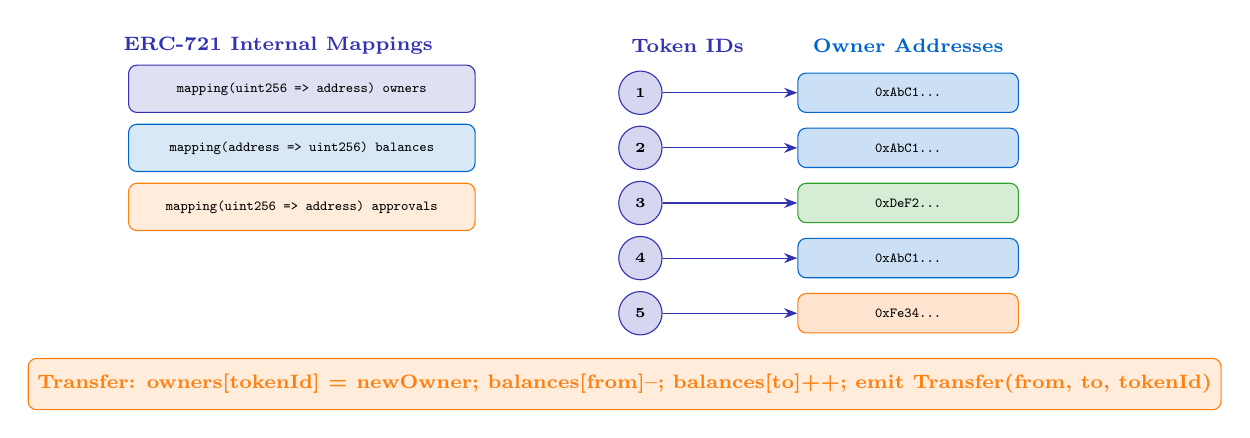
\begin{tikzpicture}[remember picture]
  %--- Data structures ---
  \node[font=\scriptsize\bfseries, text=mlpurple] at (1.6,5.3) {ERC-721 Internal Mappings};

  \node[draw=mlpurple, fill=mlpurple!15, rounded corners=3pt, minimum width=4.4cm, minimum height=0.6cm, font=\tiny\ttfamily, align=center] at (1.9,4.75) {mapping(uint256 => address) owners};
  \node[draw=mlblue, fill=mlblue!15, rounded corners=3pt, minimum width=4.4cm, minimum height=0.6cm, font=\tiny\ttfamily, align=center] at (1.9,4.0) {mapping(address => uint256) balances};
  \node[draw=mlorange, fill=mlorange!15, rounded corners=3pt, minimum width=4.4cm, minimum height=0.6cm, font=\tiny\ttfamily, align=center] at (1.9,3.25) {mapping(uint256 => address) approvals};

  %--- Token IDs ---
  \node[font=\scriptsize\bfseries, text=mlpurple] at (6.8,5.3) {Token IDs};
  \node[draw=mlpurple, fill=mlpurple!20, circle, minimum size=0.55cm, font=\tiny\bfseries] (t1) at (6.2,4.7) {1};
  \node[draw=mlpurple, fill=mlpurple!20, circle, minimum size=0.55cm, font=\tiny\bfseries] (t2) at (6.2,4.0) {2};
  \node[draw=mlpurple, fill=mlpurple!20, circle, minimum size=0.55cm, font=\tiny\bfseries] (t3) at (6.2,3.3) {3};
  \node[draw=mlpurple, fill=mlpurple!20, circle, minimum size=0.55cm, font=\tiny\bfseries] (t4) at (6.2,2.6) {4};
  \node[draw=mlpurple, fill=mlpurple!20, circle, minimum size=0.55cm, font=\tiny\bfseries] (t5) at (6.2,1.9) {5};

  %--- Owner addresses ---
  \node[font=\scriptsize\bfseries, text=mlblue] at (9.6,5.3) {Owner Addresses};
  \node[draw=mlblue, fill=mlblue!20, rounded corners=3pt, minimum width=2.8cm, minimum height=0.5cm, font=\tiny\ttfamily, align=center] (a1) at (9.6,4.7) {0xAbC1...};
  \node[draw=mlblue, fill=mlblue!20, rounded corners=3pt, minimum width=2.8cm, minimum height=0.5cm, font=\tiny\ttfamily, align=center] (a2) at (9.6,4.0) {0xAbC1...};
  \node[draw=mlgreen, fill=mlgreen!20, rounded corners=3pt, minimum width=2.8cm, minimum height=0.5cm, font=\tiny\ttfamily, align=center] (a3) at (9.6,3.3) {0xDeF2...};
  \node[draw=mlblue, fill=mlblue!20, rounded corners=3pt, minimum width=2.8cm, minimum height=0.5cm, font=\tiny\ttfamily, align=center] (a4) at (9.6,2.6) {0xAbC1...};
  \node[draw=mlorange, fill=mlorange!20, rounded corners=3pt, minimum width=2.8cm, minimum height=0.5cm, font=\tiny\ttfamily, align=center] (a5) at (9.6,1.9) {0xFe34...};

  % Arrows tokenId -> owner
  \draw[-{Stealth}, mlpurple, thin] (t1.east) -- (a1.west);
  \draw[-{Stealth}, mlpurple, thin] (t2.east) -- (a2.west);
  \draw[-{Stealth}, mlpurple, thin] (t3.east) -- (a3.west);
  \draw[-{Stealth}, mlpurple, thin] (t4.east) -- (a4.west);
  \draw[-{Stealth}, mlpurple, thin] (t5.east) -- (a5.west);

  % Transfer flow note
  \node[draw=mlorange, fill=mlorange!15, rounded corners=3pt, minimum width=11.5cm, minimum height=0.65cm, font=\scriptsize\bfseries, align=center, text=mlorange] at (6.0,1.0) {Transfer: owners[tokenId] = newOwner; balances[from]--; balances[to]++; emit Transfer(from, to, tokenId)};
\end{tikzpicture}
\bottomnote{An NFT contract is fundamentally a mapping from token IDs to owner addresses}
\end{frame}

% Frame 13: NFT Minting Process
\begin{frame}{NFT Minting Process}
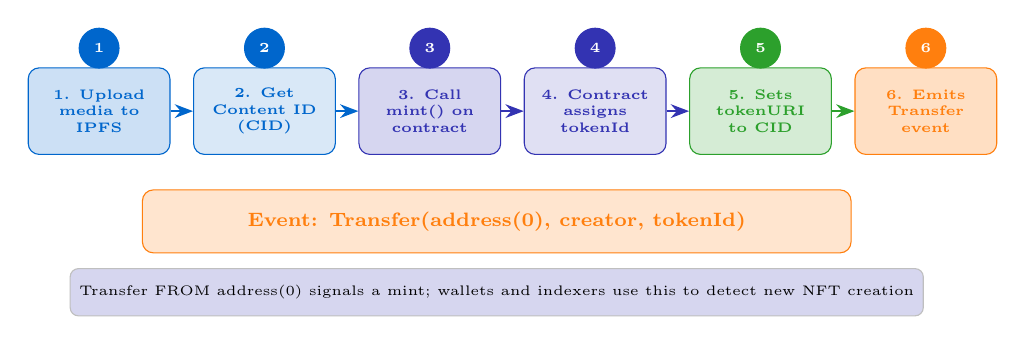
\begin{tikzpicture}[remember picture]
  % Step nodes
  \node[draw=mlblue, fill=mlblue!20, rounded corners=4pt, minimum width=1.8cm, minimum height=1.1cm, font=\tiny\bfseries, align=center, text=mlblue] (s1) at (0.95,3.5) {1. Upload\\media to\\IPFS};
  \node[draw=mlblue, fill=mlblue!15, rounded corners=4pt, minimum width=1.8cm, minimum height=1.1cm, font=\tiny\bfseries, align=center, text=mlblue] (s2) at (3.05,3.5) {2. Get\\Content ID\\(CID)};
  \node[draw=mlpurple, fill=mlpurple!20, rounded corners=4pt, minimum width=1.8cm, minimum height=1.1cm, font=\tiny\bfseries, align=center, text=mlpurple] (s3) at (5.15,3.5) {3. Call\\mint() on\\contract};
  \node[draw=mlpurple, fill=mlpurple!15, rounded corners=4pt, minimum width=1.8cm, minimum height=1.1cm, font=\tiny\bfseries, align=center, text=mlpurple] (s4) at (7.25,3.5) {4. Contract\\assigns\\tokenId};
  \node[draw=mlgreen, fill=mlgreen!20, rounded corners=4pt, minimum width=1.8cm, minimum height=1.1cm, font=\tiny\bfseries, align=center, text=mlgreen] (s5) at (9.35,3.5) {5. Sets\\tokenURI\\to CID};
  \node[draw=mlorange, fill=mlorange!25, rounded corners=4pt, minimum width=1.8cm, minimum height=1.1cm, font=\tiny\bfseries, align=center, text=mlorange] (s6) at (11.45,3.5) {6. Emits\\Transfer\\event};

  % Arrows between steps
  \draw[-{Stealth}, thick, mlblue] (s1.east) -- (s2.west);
  \draw[-{Stealth}, thick, mlblue] (s2.east) -- (s3.west);
  \draw[-{Stealth}, thick, mlpurple] (s3.east) -- (s4.west);
  \draw[-{Stealth}, thick, mlpurple] (s4.east) -- (s5.west);
  \draw[-{Stealth}, thick, mlgreen] (s5.east) -- (s6.west);

  % Step number circles
  \node[draw=mlblue, fill=mlblue, circle, minimum size=0.4cm, font=\tiny\bfseries, text=white] at (0.95,4.3) {1};
  \node[draw=mlblue, fill=mlblue, circle, minimum size=0.4cm, font=\tiny\bfseries, text=white] at (3.05,4.3) {2};
  \node[draw=mlpurple, fill=mlpurple, circle, minimum size=0.4cm, font=\tiny\bfseries, text=white] at (5.15,4.3) {3};
  \node[draw=mlpurple, fill=mlpurple, circle, minimum size=0.4cm, font=\tiny\bfseries, text=white] at (7.25,4.3) {4};
  \node[draw=mlgreen, fill=mlgreen, circle, minimum size=0.4cm, font=\tiny\bfseries, text=white] at (9.35,4.3) {5};
  \node[draw=mlorange, fill=mlorange, circle, minimum size=0.4cm, font=\tiny\bfseries, text=white] at (11.45,4.3) {6};

  % Event highlight box
  \node[draw=mlorange, fill=mlorange!20, rounded corners=4pt, minimum width=9.0cm, minimum height=0.8cm, font=\scriptsize\bfseries, align=center, text=mlorange] at (6.0,2.1) {Event: Transfer(address(0), creator, tokenId)};

  % Explanation
  \node[draw=mlgray!50, fill=mllavender4, rounded corners=3pt, minimum width=9.0cm, minimum height=0.6cm, font=\tiny, align=center] at (6.0,1.2) {Transfer FROM address(0) signals a mint; wallets and indexers use this to detect new NFT creation};
\end{tikzpicture}
\bottomnote{Minting emits a Transfer event from the zero address -- this is how wallets detect new NFTs}
\end{frame}

% Frame 14: Section 1 Summary
\begin{frame}{Section 1 Summary}
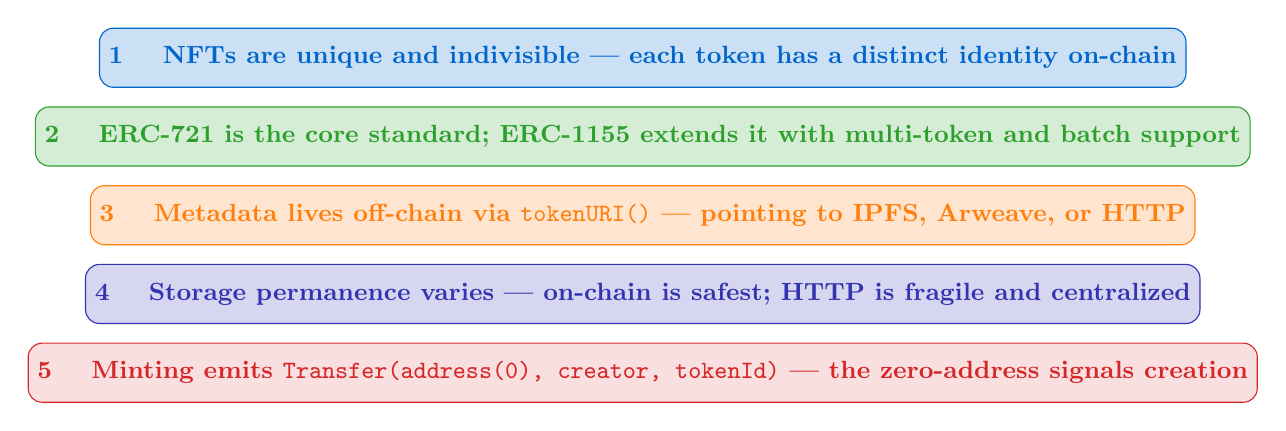
\begin{tikzpicture}[remember picture]
  \node[draw=mlblue, fill=mlblue!20, rounded corners=5pt, minimum width=11.6cm, minimum height=0.75cm, font=\small\bfseries, align=center, text=mlblue] at (6.0,5.2) {1 \quad NFTs are unique and indivisible --- each token has a distinct identity on-chain};
  \node[draw=mlgreen, fill=mlgreen!20, rounded corners=5pt, minimum width=11.6cm, minimum height=0.75cm, font=\small\bfseries, align=center, text=mlgreen] at (6.0,4.2) {2 \quad ERC-721 is the core standard; ERC-1155 extends it with multi-token and batch support};
  \node[draw=mlorange, fill=mlorange!20, rounded corners=5pt, minimum width=11.6cm, minimum height=0.75cm, font=\small\bfseries, align=center, text=mlorange] at (6.0,3.2) {3 \quad Metadata lives off-chain via \texttt{tokenURI()} --- pointing to IPFS, Arweave, or HTTP};
  \node[draw=mlpurple, fill=mlpurple!20, rounded corners=5pt, minimum width=11.6cm, minimum height=0.75cm, font=\small\bfseries, align=center, text=mlpurple] at (6.0,2.2) {4 \quad Storage permanence varies --- on-chain is safest; HTTP is fragile and centralized};
  \node[draw=mlred, fill=mlred!15, rounded corners=5pt, minimum width=11.6cm, minimum height=0.75cm, font=\small\bfseries, align=center, text=mlred] at (6.0,1.2) {5 \quad Minting emits \texttt{Transfer(address(0), creator, tokenId)} --- the zero-address signals creation};
\end{tikzpicture}
\bottomnote{Section 1 complete -- next: NFT Marketplaces \& Trading}
\end{frame}

%% ============================================================
%% SECTION 2: NFT MARKETPLACES & TRADING
%% ============================================================
\section{NFT Marketplaces \& Trading}

% Frame 15: Section 2 Divider
\begin{frame}{Section 2: NFT Marketplaces \& Trading}
\begin{beamercolorbox}[sep=12pt,center,rounded=true,shadow=true]{palette quaternary}
  {\Large\bfseries Section 2: NFT Marketplaces \& Trading}\\[4pt]
  {\normalsize Platforms, pricing mechanics, royalties, and market structure}
\end{beamercolorbox}

\vspace{4mm}
\begin{columns}[T]
\column{0.55\textwidth}
\begin{block}{What You Will Learn}
\begin{itemize}\setlength{\itemsep}{2pt}
  \item How NFT marketplace ecosystems are structured
  \item Mechanics of on-chain NFT trading and settlement
  \item Pricing models: fixed price, English and Dutch auctions
  \item Creator royalties and the EIP-2981 standard
  \item Floor price, wash trading, and market integrity
\end{itemize}
\end{block}
\column{0.42\textwidth}
\begin{block}{Frames in This Section}
\begin{itemize}\setlength{\itemsep}{1pt}
  \item Frame 15 --- Section overview
  \item Frame 16 --- Marketplace landscape
  \item Frame 17 --- How NFT trading works
  \item Frame 18 --- Pricing mechanisms
  \item Frame 19 --- Royalty mechanics
  \item Frame 20 --- Fee comparison
  \item Frame 21 --- Floor price mechanics
  \item Frame 22 --- Order book vs AMM
  \item Frame 23 --- NFT lending
  \item Frame 24 --- Wash trading
  \item Frame 25 --- Gas costs \& Layer-2
  \item Frame 26 --- Section 2 summary
\end{itemize}
\end{block}
\end{columns}
\bottomnote{Section 2 | Frames 15--26 | NFT Marketplaces \& Trading}
\end{frame}

% Frame 16: NFT Marketplace Landscape
\begin{frame}{NFT Marketplace Landscape}
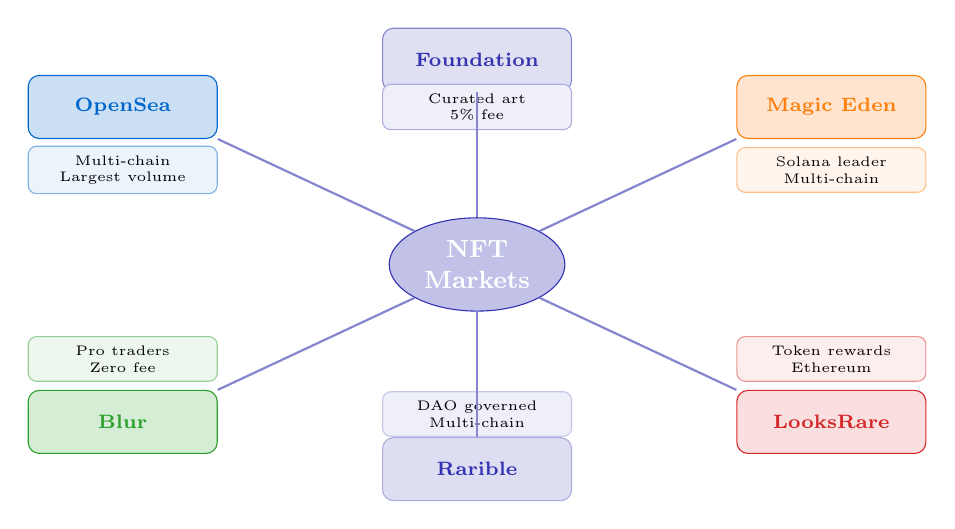
\begin{tikzpicture}[remember picture]
  % Center node
  \node[draw=mlpurple, fill=mlpurple!30, ellipse, minimum width=2.2cm, minimum height=1.0cm, font=\small\bfseries, align=center, text=white] (center) at (6.0,3.0) {NFT\\Markets};

  % OpenSea
  \node[draw=mlblue, fill=mlblue!20, rounded corners=4pt, minimum width=2.4cm, minimum height=0.8cm, font=\scriptsize\bfseries, align=center, text=mlblue] (opensea) at (1.5,5.0) {OpenSea};
  \node[draw=mlblue!50, fill=mlblue!8, rounded corners=3pt, minimum width=2.4cm, minimum height=0.55cm, font=\tiny, align=center] (opensea2) at (1.5,4.2) {Multi-chain\\Largest volume};

  % Blur
  \node[draw=mlgreen, fill=mlgreen!20, rounded corners=4pt, minimum width=2.4cm, minimum height=0.8cm, font=\scriptsize\bfseries, align=center, text=mlgreen] (blur) at (1.5,1.0) {Blur};
  \node[draw=mlgreen!50, fill=mlgreen!8, rounded corners=3pt, minimum width=2.4cm, minimum height=0.55cm, font=\tiny, align=center] (blur2) at (1.5,1.8) {Pro traders\\Zero fee};

  % Magic Eden
  \node[draw=mlorange, fill=mlorange!20, rounded corners=4pt, minimum width=2.4cm, minimum height=0.8cm, font=\scriptsize\bfseries, align=center, text=mlorange] (magic) at (10.5,5.0) {Magic Eden};
  \node[draw=mlorange!50, fill=mlorange!8, rounded corners=3pt, minimum width=2.4cm, minimum height=0.55cm, font=\tiny, align=center] (magic2) at (10.5,4.2) {Solana leader\\Multi-chain};

  % LooksRare
  \node[draw=mlred, fill=mlred!15, rounded corners=4pt, minimum width=2.4cm, minimum height=0.8cm, font=\scriptsize\bfseries, align=center, text=mlred] (looks) at (10.5,1.0) {LooksRare};
  \node[draw=mlred!50, fill=mlred!8, rounded corners=3pt, minimum width=2.4cm, minimum height=0.55cm, font=\tiny, align=center] (looks2) at (10.5,1.8) {Token rewards\\Ethereum};

  % Foundation
  \node[draw=mlpurple!60, fill=mlpurple!15, rounded corners=4pt, minimum width=2.4cm, minimum height=0.8cm, font=\scriptsize\bfseries, align=center, text=mlpurple] (found) at (6.0,5.6) {Foundation};
  \node[draw=mlpurple!40, fill=mlpurple!8, rounded corners=3pt, minimum width=2.4cm, minimum height=0.55cm, font=\tiny, align=center] (found2) at (6.0,5.0) {Curated art\\5\% fee};

  % Rarible
  \node[draw=mllavender, fill=mllavender!40, rounded corners=4pt, minimum width=2.4cm, minimum height=0.8cm, font=\scriptsize\bfseries, align=center, text=mlpurple] (rarible) at (6.0,0.4) {Rarible};
  \node[draw=mllavender!70, fill=mllavender!20, rounded corners=3pt, minimum width=2.4cm, minimum height=0.55cm, font=\tiny, align=center] (rarible2) at (6.0,1.1) {DAO governed\\Multi-chain};

  % Spokes from center
  \draw[thick, mlpurple!60] (center.north west) -- (opensea.south east);
  \draw[thick, mlpurple!60] (center.south west) -- (blur.north east);
  \draw[thick, mlpurple!60] (center.north east) -- (magic.south west);
  \draw[thick, mlpurple!60] (center.south east) -- (looks.north west);
  \draw[thick, mlpurple!60] (center.north) -- (found.south);
  \draw[thick, mlpurple!60] (center.south) -- (rarible.north);
\end{tikzpicture}
\bottomnote{The NFT marketplace landscape has shifted from OpenSea dominance to competitive multi-platform trading}
\end{frame}

% Frame 17: How NFT Trading Works
\begin{frame}{How NFT Trading Works}
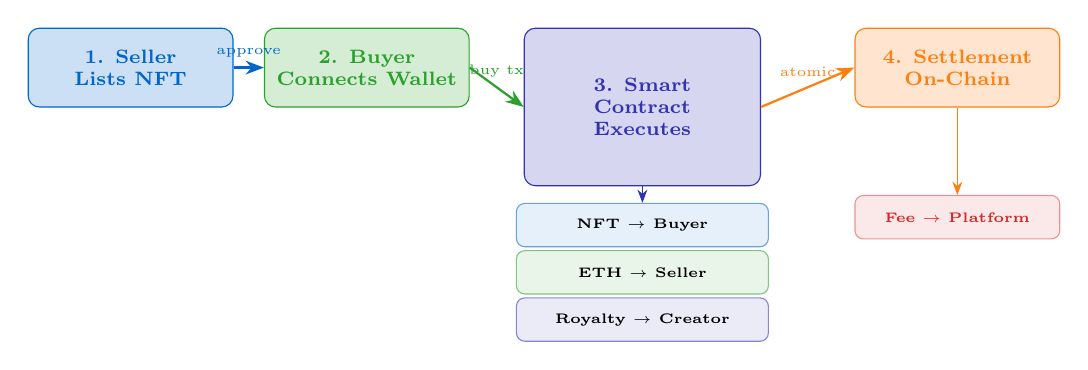
\begin{tikzpicture}[remember picture]
  % Step 1: Seller lists
  \node[draw=mlblue, fill=mlblue!20, rounded corners=4pt, minimum width=2.6cm, minimum height=1.0cm, font=\scriptsize\bfseries, align=center, text=mlblue] (list) at (0.5,3.5) {1. Seller\\Lists NFT};

  % Step 2: Buyer connects
  \node[draw=mlgreen, fill=mlgreen!20, rounded corners=4pt, minimum width=2.6cm, minimum height=1.0cm, font=\scriptsize\bfseries, align=center, text=mlgreen] (connect) at (3.5,3.5) {2. Buyer\\Connects Wallet};

  % Step 3: Smart contract
  \node[draw=mlpurple, fill=mlpurple!20, rounded corners=4pt, minimum width=3.0cm, minimum height=2.0cm, font=\scriptsize\bfseries, align=center, text=mlpurple] (sc) at (7.0,3.0) {3. Smart\\Contract\\Executes};

  % Step 4: Settlement
  \node[draw=mlorange, fill=mlorange!20, rounded corners=4pt, minimum width=2.6cm, minimum height=1.0cm, font=\scriptsize\bfseries, align=center, text=mlorange] (settle) at (11.0,3.5) {4. Settlement\\On-Chain};

  % Arrows
  \draw[-{Stealth}, thick, mlblue] (list.east) -- node[above, font=\tiny] {approve} (connect.west);
  \draw[-{Stealth}, thick, mlgreen] (connect.east) -- node[above, font=\tiny] {buy tx} (sc.west);
  \draw[-{Stealth}, thick, mlorange] (sc.east) -- node[above, font=\tiny] {atomic} (settle.west);

  % Smart contract outputs
  \node[draw=mlblue!60, fill=mlblue!10, rounded corners=3pt, minimum width=3.2cm, minimum height=0.55cm, font=\tiny\bfseries, align=center] (nfttob) at (7.0,1.5) {NFT $\to$ Buyer};
  \node[draw=mlgreen!60, fill=mlgreen!10, rounded corners=3pt, minimum width=3.2cm, minimum height=0.55cm, font=\tiny\bfseries, align=center] (ethtosell) at (7.0,0.9) {ETH $\to$ Seller};
  \node[draw=mlpurple!60, fill=mlpurple!10, rounded corners=3pt, minimum width=3.2cm, minimum height=0.55cm, font=\tiny\bfseries, align=center] (roytocreate) at (7.0,0.3) {Royalty $\to$ Creator};

  \draw[-{Stealth}, thin, mlpurple] (sc.south) -- (nfttob.north);

  % Platform fee note
  \node[draw=mlred!50, fill=mlred!10, rounded corners=3pt, minimum width=2.6cm, minimum height=0.55cm, font=\tiny\bfseries, align=center, text=mlred] (fee) at (11.0,1.6) {Fee $\to$ Platform};
  \draw[-{Stealth}, thin, mlorange] (settle.south) -- (fee.north);
\end{tikzpicture}
\bottomnote{NFT trades are atomic on-chain transactions -- payment and delivery happen simultaneously}
\end{frame}

% Frame 18: Pricing Mechanisms
\begin{frame}{Pricing Mechanisms}
\begin{columns}[T]
\column{0.32\textwidth}
\begin{block}{Fixed Price}
\begin{itemize}\setlength{\itemsep}{2pt}
  \item Seller sets a price
  \item First buyer pays and receives NFT
  \item No time pressure
  \item Simple and predictable
\end{itemize}
\end{block}
\vspace{2mm}
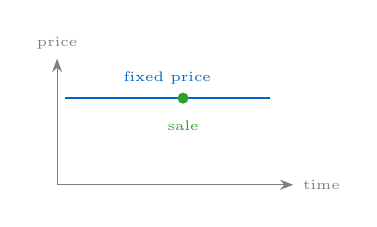
\begin{tikzpicture}[remember picture]
  \draw[-{Stealth}, thin, mlgray] (0,0) -- (3.0,0) node[right, font=\tiny] {time};
  \draw[-{Stealth}, thin, mlgray] (0,0) -- (0,1.6) node[above, font=\tiny] {price};
  \draw[thick, mlblue] (0.1,1.1) -- (2.7,1.1);
  \node[font=\tiny, text=mlblue] at (1.4,1.35) {fixed price};
  \fill[mlgreen] (1.6,1.1) circle (2pt);
  \node[font=\tiny, text=mlgreen] at (1.6,0.75) {sale};
\end{tikzpicture}

\column{0.32\textwidth}
\begin{block}{English Auction}
\begin{itemize}\setlength{\itemsep}{2pt}
  \item Ascending bid competition
  \item Highest bid wins at close
  \item Creates urgency and FOMO
  \item Price discovery via demand
\end{itemize}
\end{block}
\vspace{2mm}
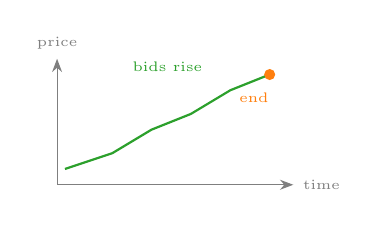
\begin{tikzpicture}[remember picture]
  \draw[-{Stealth}, thin, mlgray] (0,0) -- (3.0,0) node[right, font=\tiny] {time};
  \draw[-{Stealth}, thin, mlgray] (0,0) -- (0,1.6) node[above, font=\tiny] {price};
  \draw[thick, mlgreen] (0.1,0.2) -- (0.7,0.4) -- (1.2,0.7) -- (1.7,0.9) -- (2.2,1.2) -- (2.7,1.4);
  \node[font=\tiny, text=mlgreen] at (1.4,1.5) {bids rise};
  \fill[mlorange] (2.7,1.4) circle (2pt);
  \node[font=\tiny, text=mlorange] at (2.5,1.1) {end};
\end{tikzpicture}

\column{0.32\textwidth}
\begin{block}{Dutch Auction}
\begin{itemize}\setlength{\itemsep}{2pt}
  \item Price starts high, falls over time
  \item First buyer to accept wins
  \item Fair price discovery for mints
  \item Popular for large collections
\end{itemize}
\end{block}
\vspace{2mm}
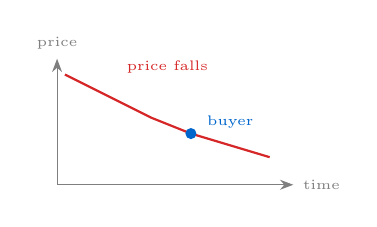
\begin{tikzpicture}[remember picture]
  \draw[-{Stealth}, thin, mlgray] (0,0) -- (3.0,0) node[right, font=\tiny] {time};
  \draw[-{Stealth}, thin, mlgray] (0,0) -- (0,1.6) node[above, font=\tiny] {price};
  \draw[thick, mlred] (0.1,1.4) -- (0.7,1.1) -- (1.2,0.85) -- (1.7,0.65) -- (2.2,0.5) -- (2.7,0.35);
  \node[font=\tiny, text=mlred] at (1.4,1.5) {price falls};
  \fill[mlblue] (1.7,0.65) circle (2pt);
  \node[font=\tiny, text=mlblue] at (2.2,0.8) {buyer};
\end{tikzpicture}
\end{columns}
\bottomnote{Dutch auctions are popular for NFT mints because they help discover fair market price}
\end{frame}

% Frame 19: NFT Royalty Mechanics [FRAGILE]
\begin{frame}[fragile]{NFT Royalty Mechanics}
\begin{columns}[T]
\column{0.46\textwidth}
\begin{block}{Creator Royalties}
\begin{itemize}\setlength{\itemsep}{2pt}
  \item Royalties give creators a \% of every secondary sale
  \item Typically 5--10\% of sale price
  \item Paid automatically by marketplace smart contracts
  \item \textbf{EIP-2981} standardizes royalty queries on-chain
\end{itemize}
\end{block}
\vspace{3mm}
\begin{block}{Enforcement Challenges}
\begin{itemize}\setlength{\itemsep}{2pt}
  \item EIP-2981 only \textit{declares} royalties --- cannot enforce
  \item Marketplaces may choose to ignore royalty info
  \item \textbf{Royalty wars (2022--23):} Blur made royalties optional
  \item Creator revenue fell significantly as a result
  \item Some projects use transfer restrictions to enforce
\end{itemize}
\end{block}

\column{0.51\textwidth}
\begin{lstlisting}[language=Solidity]
// EIP-2981 Royalty Standard
interface IERC2981 {
    function royaltyInfo(
        uint256 tokenId,
        uint256 salePrice
    ) external view returns (
        address receiver,
        uint256 royaltyAmount
    );
}
// Example: 5% royalty
// salePrice = 1 ether
// royaltyAmount = 0.05 ether
\end{lstlisting}
\end{columns}
\bottomnote{EIP-2981 standardizes royalty queries but enforcement depends on marketplace cooperation}
\end{frame}

% Frame 20: Marketplace Fee Comparison
\begin{frame}{Marketplace Fee Comparison}
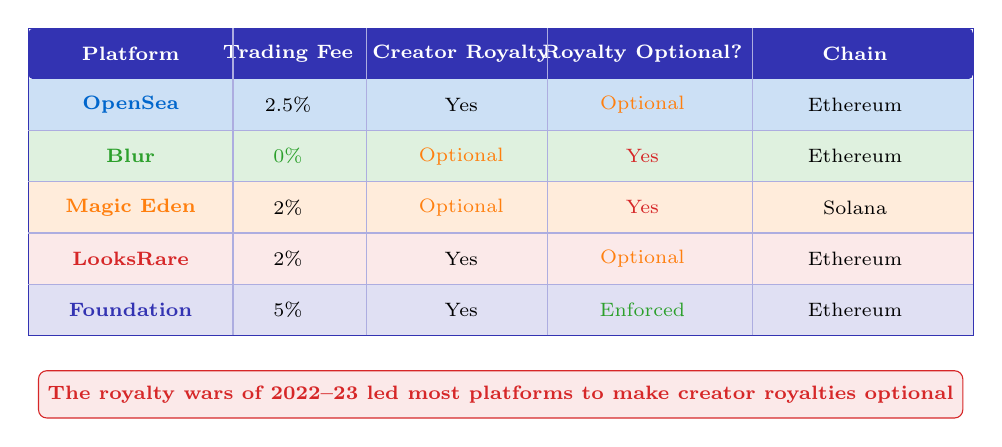
\begin{tikzpicture}[remember picture]
  % Header
  \fill[mlpurple, rounded corners=2pt] (0,5.1) rectangle (12.0,5.75);
  \node[font=\scriptsize\bfseries, text=white, align=center] at (1.3,5.425) {Platform};
  \node[font=\scriptsize\bfseries, text=white, align=center] at (3.3,5.425) {Trading Fee};
  \node[font=\scriptsize\bfseries, text=white, align=center] at (5.5,5.425) {Creator Royalty};
  \node[font=\scriptsize\bfseries, text=white, align=center] at (7.8,5.425) {Royalty Optional?};
  \node[font=\scriptsize\bfseries, text=white, align=center] at (10.5,5.425) {Chain};

  % Row 1: OpenSea
  \fill[mlblue!20] (0,4.45) rectangle (12.0,5.1);
  \node[font=\scriptsize\bfseries, text=mlblue, align=center] at (1.3,4.775) {OpenSea};
  \node[font=\scriptsize, align=center] at (3.3,4.775) {2.5\%};
  \node[font=\scriptsize, align=center] at (5.5,4.775) {Yes};
  \node[font=\scriptsize, text=mlorange, align=center] at (7.8,4.775) {Optional};
  \node[font=\scriptsize, align=center] at (10.5,4.775) {Ethereum};

  % Row 2: Blur
  \fill[mlgreen!15] (0,3.8) rectangle (12.0,4.45);
  \node[font=\scriptsize\bfseries, text=mlgreen, align=center] at (1.3,4.125) {Blur};
  \node[font=\scriptsize, text=mlgreen, align=center] at (3.3,4.125) {0\%};
  \node[font=\scriptsize, text=mlorange, align=center] at (5.5,4.125) {Optional};
  \node[font=\scriptsize, text=mlred, align=center] at (7.8,4.125) {Yes};
  \node[font=\scriptsize, align=center] at (10.5,4.125) {Ethereum};

  % Row 3: Magic Eden
  \fill[mlorange!15] (0,3.15) rectangle (12.0,3.8);
  \node[font=\scriptsize\bfseries, text=mlorange, align=center] at (1.3,3.475) {Magic Eden};
  \node[font=\scriptsize, align=center] at (3.3,3.475) {2\%};
  \node[font=\scriptsize, text=mlorange, align=center] at (5.5,3.475) {Optional};
  \node[font=\scriptsize, text=mlred, align=center] at (7.8,3.475) {Yes};
  \node[font=\scriptsize, align=center] at (10.5,3.475) {Solana};

  % Row 4: LooksRare
  \fill[mlred!10] (0,2.5) rectangle (12.0,3.15);
  \node[font=\scriptsize\bfseries, text=mlred, align=center] at (1.3,2.825) {LooksRare};
  \node[font=\scriptsize, align=center] at (3.3,2.825) {2\%};
  \node[font=\scriptsize, align=center] at (5.5,2.825) {Yes};
  \node[font=\scriptsize, text=mlorange, align=center] at (7.8,2.825) {Optional};
  \node[font=\scriptsize, align=center] at (10.5,2.825) {Ethereum};

  % Row 5: Foundation
  \fill[mlpurple!15] (0,1.85) rectangle (12.0,2.5);
  \node[font=\scriptsize\bfseries, text=mlpurple, align=center] at (1.3,2.175) {Foundation};
  \node[font=\scriptsize, align=center] at (3.3,2.175) {5\%};
  \node[font=\scriptsize, align=center] at (5.5,2.175) {Yes};
  \node[font=\scriptsize, text=mlgreen, align=center] at (7.8,2.175) {Enforced};
  \node[font=\scriptsize, align=center] at (10.5,2.175) {Ethereum};

  % Table border and column lines
  \draw[mlpurple, thin] (0,1.85) rectangle (12.0,5.75);
  \draw[mlpurple!40, thin] (2.6,1.85) -- (2.6,5.75);
  \draw[mlpurple!40, thin] (4.3,1.85) -- (4.3,5.75);
  \draw[mlpurple!40, thin] (6.6,1.85) -- (6.6,5.75);
  \draw[mlpurple!40, thin] (9.2,1.85) -- (9.2,5.75);
  \draw[mlpurple!40, thin] (0,2.5) -- (12.0,2.5);
  \draw[mlpurple!40, thin] (0,3.15) -- (12.0,3.15);
  \draw[mlpurple!40, thin] (0,3.8) -- (12.0,3.8);
  \draw[mlpurple!40, thin] (0,4.45) -- (12.0,4.45);

  % Note
  \node[draw=mlred, fill=mlred!10, rounded corners=3pt, minimum width=11.6cm, minimum height=0.6cm, font=\scriptsize\bfseries, align=center, text=mlred] at (6.0,1.1) {The royalty wars of 2022--23 led most platforms to make creator royalties optional};
\end{tikzpicture}
\bottomnote{The royalty wars of 2022--23 led most platforms to make creator royalties optional}
\end{frame}

% Frame 21: Floor Price Mechanics
\begin{frame}{Floor Price Mechanics}
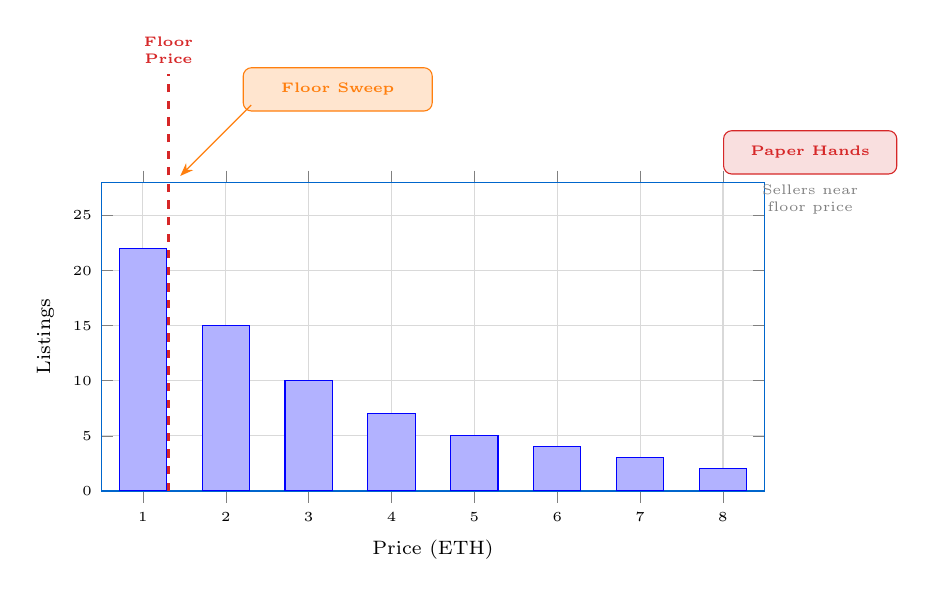
\begin{tikzpicture}[remember picture]
  \begin{axis}[
    at={(0.5cm,0.5cm)},
    width=10cm,
    height=5.5cm,
    xlabel={Price (ETH)},
    ylabel={Listings},
    xlabel style={font=\scriptsize},
    ylabel style={font=\scriptsize},
    xtick={1,2,3,4,5,6,7,8},
    xticklabels={1,2,3,4,5,6,7,8},
    ytick={0,5,10,15,20,25},
    tick label style={font=\tiny},
    ymin=0, ymax=28,
    xmin=0.5, xmax=8.5,
    grid=major,
    grid style={mlgray!30},
    bar width=0.6cm,
    ybar,
    fill=mlblue!50,
    draw=mlblue,
  ]
    \addplot coordinates {
      (1,22) (2,15) (3,10) (4,7) (5,5) (6,4) (7,3) (8,2)
    };
  \end{axis}
  % Floor price annotation
  \draw[dashed, mlred, very thick] (1.35,0.5) -- (1.35,5.8);
  \node[font=\tiny\bfseries, text=mlred, align=center] at (1.35,6.1) {Floor\\Price};
  % Annotations
  \node[draw=mlorange, fill=mlorange!20, rounded corners=3pt, minimum width=2.4cm, minimum height=0.55cm, font=\tiny\bfseries, align=center, text=mlorange] at (3.5,5.6) {Floor Sweep};
  \draw[-{Stealth}, thin, mlorange] (2.4,5.4) -- (1.5,4.5);
  \node[draw=mlred, fill=mlred!15, rounded corners=3pt, minimum width=2.2cm, minimum height=0.55cm, font=\tiny\bfseries, align=center, text=mlred] at (9.5,4.8) {Paper Hands};
  \node[font=\tiny, text=mlgray, align=center] at (9.5,4.2) {Sellers near\\floor price};
\end{tikzpicture}
\bottomnote{Floor price is the minimum entry cost for a collection -- it is the most-watched metric in NFT trading}
\end{frame}

% Frame 22: Order Book vs AMM for NFTs
\begin{frame}{Order Book vs AMM for NFTs}
\begin{columns}[T]
\column{0.47\textwidth}
\begin{block}{Traditional Order Book (OpenSea)}
\end{block}
\vspace{1mm}
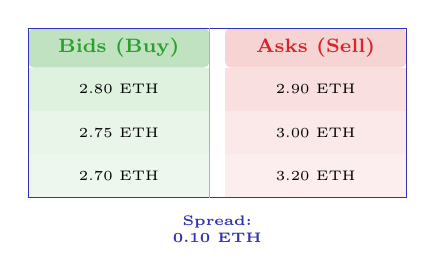
\begin{tikzpicture}[remember picture]
  % Bids column header
  \fill[mlgreen!30, rounded corners=2pt] (0,3.3) rectangle (2.3,3.8);
  \node[font=\scriptsize\bfseries, text=mlgreen] at (1.15,3.55) {Bids (Buy)};
  % Ask column header
  \fill[mlred!20, rounded corners=2pt] (2.5,3.3) rectangle (4.8,3.8);
  \node[font=\scriptsize\bfseries, text=mlred] at (3.65,3.55) {Asks (Sell)};
  % Bid rows
  \fill[mlgreen!15] (0,2.75) rectangle (2.3,3.3);
  \node[font=\tiny, align=center] at (1.15,3.025) {2.80 ETH};
  \fill[mlgreen!10] (0,2.2) rectangle (2.3,2.75);
  \node[font=\tiny, align=center] at (1.15,2.475) {2.75 ETH};
  \fill[mlgreen!8] (0,1.65) rectangle (2.3,2.2);
  \node[font=\tiny, align=center] at (1.15,1.925) {2.70 ETH};
  % Ask rows
  \fill[mlred!15] (2.5,2.75) rectangle (4.8,3.3);
  \node[font=\tiny, align=center] at (3.65,3.025) {2.90 ETH};
  \fill[mlred!10] (2.5,2.2) rectangle (4.8,2.75);
  \node[font=\tiny, align=center] at (3.65,2.475) {3.00 ETH};
  \fill[mlred!8] (2.5,1.65) rectangle (4.8,2.2);
  \node[font=\tiny, align=center] at (3.65,1.925) {3.20 ETH};
  % Spread label
  \node[font=\tiny\bfseries, text=mlpurple, align=center] at (2.4,1.25) {Spread:\\0.10 ETH};
  \draw[mlpurple, thin] (0,1.65) rectangle (4.8,3.8);
  \draw[mlpurple!40, thin] (2.3,1.65) -- (2.3,3.8);
\end{tikzpicture}

\column{0.47\textwidth}
\begin{block}{AMM Model (Sudoswap)}
\end{block}
\vspace{1mm}
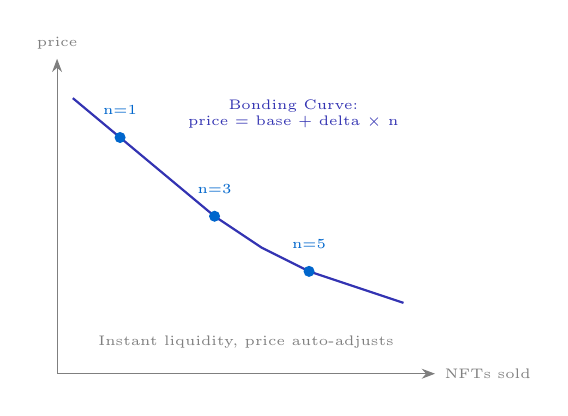
\begin{tikzpicture}[remember picture]
  \draw[-{Stealth}, thin, mlgray] (0,0) -- (4.8,0) node[right, font=\tiny] {NFTs sold};
  \draw[-{Stealth}, thin, mlgray] (0,0) -- (0,4.0) node[above, font=\tiny] {price};
  % Bonding curve
  \draw[thick, mlpurple] (0.2,3.5) -- (0.8,3.0) -- (1.4,2.5) -- (2.0,2.0) -- (2.6,1.6) -- (3.2,1.3) -- (3.8,1.1) -- (4.4,0.9);
  \node[font=\tiny, text=mlpurple, align=center] at (3.0,3.3) {Bonding Curve:\\price = base + delta $\times$ n};
  % Points on curve
  \fill[mlblue] (0.8,3.0) circle (2pt);
  \fill[mlblue] (2.0,2.0) circle (2pt);
  \fill[mlblue] (3.2,1.3) circle (2pt);
  % Labels
  \node[font=\tiny, text=mlblue, align=center] at (0.8,3.35) {n=1};
  \node[font=\tiny, text=mlblue, align=center] at (2.0,2.35) {n=3};
  \node[font=\tiny, text=mlblue, align=center] at (3.2,1.65) {n=5};
  \node[font=\tiny, text=mlgray, align=center] at (2.4,0.4) {Instant liquidity, price auto-adjusts};
\end{tikzpicture}
\end{columns}
\bottomnote{NFT AMMs like Sudoswap bring instant liquidity but work best for floor-priced items}
\end{frame}

% Frame 23: NFT Lending and Collateralization
\begin{frame}{NFT Lending and Collateralization}
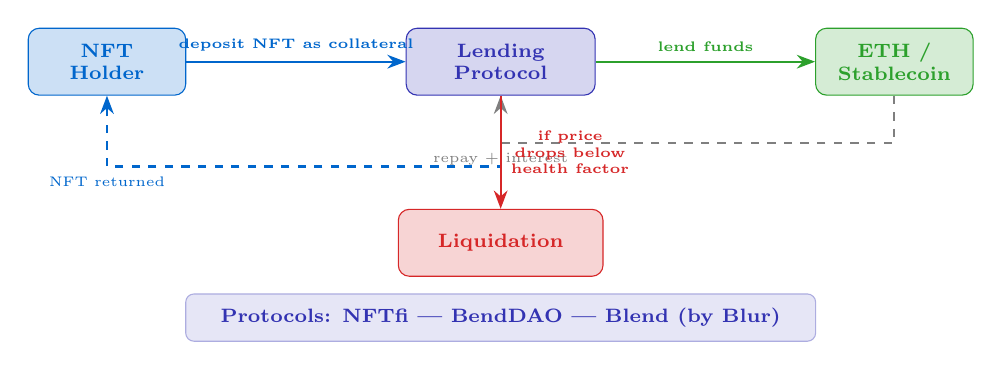
\begin{tikzpicture}[remember picture]
  % User node
  \node[draw=mlblue, fill=mlblue!20, rounded corners=4pt, minimum width=2.0cm, minimum height=0.85cm, font=\scriptsize\bfseries, align=center, text=mlblue] (user) at (1.0,3.5) {NFT\\Holder};

  % Protocol node
  \node[draw=mlpurple, fill=mlpurple!20, rounded corners=4pt, minimum width=2.4cm, minimum height=0.85cm, font=\scriptsize\bfseries, align=center, text=mlpurple] (proto) at (6.0,3.5) {Lending\\Protocol};

  % ETH/Stablecoin node
  \node[draw=mlgreen, fill=mlgreen!20, rounded corners=4pt, minimum width=2.0cm, minimum height=0.85cm, font=\scriptsize\bfseries, align=center, text=mlgreen] (eth) at (11.0,3.5) {ETH /\\Stablecoin};

  % NFT collateral
  \draw[-{Stealth}, thick, mlblue] (user.east) -- node[above, font=\tiny\bfseries] {deposit NFT as collateral} (proto.west);
  \draw[-{Stealth}, thick, mlgreen] (proto.east) -- node[above, font=\tiny\bfseries] {lend funds} (eth.west);
  \draw[-{Stealth}, thick, mlgray, dashed] (eth.south) -- ++(0,-0.6) -| node[below, font=\tiny] {repay + interest} (proto.south);
  \draw[-{Stealth}, thick, mlblue, dashed] (proto.south) -- ++(0,-0.9) -| node[below, font=\tiny] {NFT returned} (user.south);

  % Liquidation path
  \node[draw=mlred, fill=mlred!20, rounded corners=4pt, minimum width=2.6cm, minimum height=0.85cm, font=\scriptsize\bfseries, align=center, text=mlred] (liq) at (6.0,1.2) {Liquidation};
  \draw[-{Stealth}, thick, mlred] (proto.south) -- node[right, font=\tiny\bfseries, align=center] {if price\\drops below\\health factor} (liq.north);

  % Protocols box
  \node[draw=mllavender, fill=mllavender!30, rounded corners=3pt, minimum width=8.0cm, minimum height=0.6cm, font=\scriptsize\bfseries, align=center, text=mlpurple] at (6.0,0.25) {Protocols: NFTfi | BendDAO | Blend (by Blur)};
\end{tikzpicture}
\bottomnote{NFT lending unlocks liquidity for holders without selling -- but liquidation risk is significant}
\end{frame}

% Frame 24: Wash Trading Detection
\begin{frame}{Wash Trading Detection}
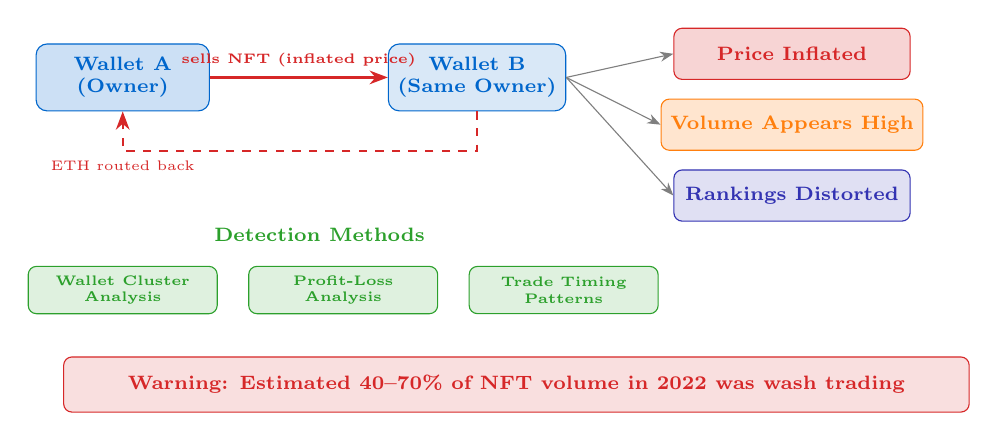
\begin{tikzpicture}[remember picture]
  % Wallet A
  \node[draw=mlblue, fill=mlblue!20, rounded corners=4pt, minimum width=2.2cm, minimum height=0.85cm, font=\scriptsize\bfseries, align=center, text=mlblue] (wA) at (1.0,4.5) {Wallet A\\(Owner)};

  % Wallet B
  \node[draw=mlblue, fill=mlblue!15, rounded corners=4pt, minimum width=2.2cm, minimum height=0.85cm, font=\scriptsize\bfseries, align=center, text=mlblue] (wB) at (5.5,4.5) {Wallet B\\(Same Owner)};

  % Arrow A to B
  \draw[-{Stealth}, thick, mlred] (wA.east) -- node[above, font=\tiny\bfseries, text=mlred] {sells NFT (inflated price)} (wB.west);
  \draw[-{Stealth}, thick, mlred, dashed] (wB.south) -- ++(0,-0.5) -| node[below, font=\tiny, text=mlred] {ETH routed back} (wA.south);

  % Effects
  \node[draw=mlred, fill=mlred!20, rounded corners=3pt, minimum width=3.0cm, minimum height=0.65cm, font=\scriptsize\bfseries, align=center, text=mlred] (eff1) at (9.5,4.8) {Price Inflated};
  \node[draw=mlorange, fill=mlorange!20, rounded corners=3pt, minimum width=3.0cm, minimum height=0.65cm, font=\scriptsize\bfseries, align=center, text=mlorange] (eff2) at (9.5,3.9) {Volume Appears High};
  \node[draw=mlpurple, fill=mlpurple!15, rounded corners=3pt, minimum width=3.0cm, minimum height=0.65cm, font=\scriptsize\bfseries, align=center, text=mlpurple] (eff3) at (9.5,3.0) {Rankings Distorted};

  \draw[-{Stealth}, thin, mlgray] (wB.east) -- (eff1.west);
  \draw[-{Stealth}, thin, mlgray] (wB.east) -- (eff2.west);
  \draw[-{Stealth}, thin, mlgray] (wB.east) -- (eff3.west);

  % Detection methods
  \node[font=\scriptsize\bfseries, text=mlgreen] at (3.5,2.5) {Detection Methods};
  \node[draw=mlgreen, fill=mlgreen!15, rounded corners=3pt, minimum width=2.4cm, minimum height=0.6cm, font=\tiny\bfseries, align=center, text=mlgreen] at (1.0,1.8) {Wallet Cluster\\Analysis};
  \node[draw=mlgreen, fill=mlgreen!15, rounded corners=3pt, minimum width=2.4cm, minimum height=0.6cm, font=\tiny\bfseries, align=center, text=mlgreen] at (3.8,1.8) {Profit-Loss\\Analysis};
  \node[draw=mlgreen, fill=mlgreen!15, rounded corners=3pt, minimum width=2.4cm, minimum height=0.6cm, font=\tiny\bfseries, align=center, text=mlgreen] at (6.6,1.8) {Trade Timing\\Patterns};

  % Warning
  \node[draw=mlred, fill=mlred!15, rounded corners=3pt, minimum width=11.5cm, minimum height=0.7cm, font=\scriptsize\bfseries, align=center, text=mlred] at (6.0,0.6) {Warning: Estimated 40--70\% of NFT volume in 2022 was wash trading};
\end{tikzpicture}
\bottomnote{Wash trading inflates volume metrics -- always verify organic trading activity before investing}
\end{frame}

% Frame 25: Gas Costs and Layer-2 NFTs
\begin{frame}{Gas Costs and Layer-2 NFTs}
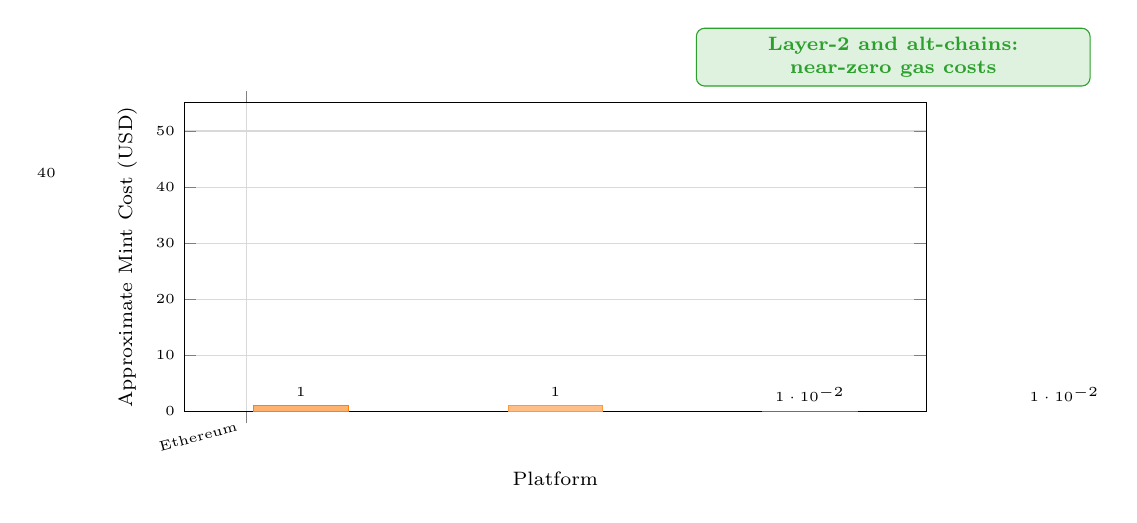
\begin{tikzpicture}[remember picture]
  \begin{axis}[
    at={(0.5cm,0.5cm)},
    width=11cm,
    height=5.5cm,
    xlabel={Platform},
    ylabel={Approximate Mint Cost (USD)},
    xlabel style={font=\scriptsize},
    ylabel style={font=\scriptsize},
    symbolic x coords={Ethereum,Arbitrum,Optimism,Polygon,Solana},
    xtick=data,
    xticklabel style={font=\tiny, rotate=15, anchor=east},
    ytick={0,10,20,30,40,50},
    tick label style={font=\tiny},
    ymin=0, ymax=55,
    ybar,
    bar width=1.2cm,
    grid=major,
    grid style={mlgray!30},
    nodes near coords,
    nodes near coords style={font=\tiny\bfseries},
  ]
    \addplot[fill=mlred!60, draw=mlred] coordinates {
      (Ethereum,40)
    };
    \addplot[fill=mlorange!60, draw=mlorange] coordinates {
      (Arbitrum,1)
    };
    \addplot[fill=mlorange!50, draw=mlorange!80] coordinates {
      (Optimism,1)
    };
    \addplot[fill=mlgreen!60, draw=mlgreen] coordinates {
      (Polygon,0.01)
    };
    \addplot[fill=mlblue!60, draw=mlblue] coordinates {
      (Solana,0.01)
    };
  \end{axis}
  % Annotation
  \node[draw=mlgreen, fill=mlgreen!15, rounded corners=3pt, minimum width=5.0cm, minimum height=0.6cm, font=\scriptsize\bfseries, align=center, text=mlgreen] at (9.5,5.0) {Layer-2 and alt-chains:\\near-zero gas costs};
\end{tikzpicture}
\bottomnote{Layer-2 and alternative chains dramatically reduce NFT gas costs, enabling mass-market adoption}
\end{frame}

% Frame 26: Section 2 Summary
\begin{frame}{Section 2 Summary}
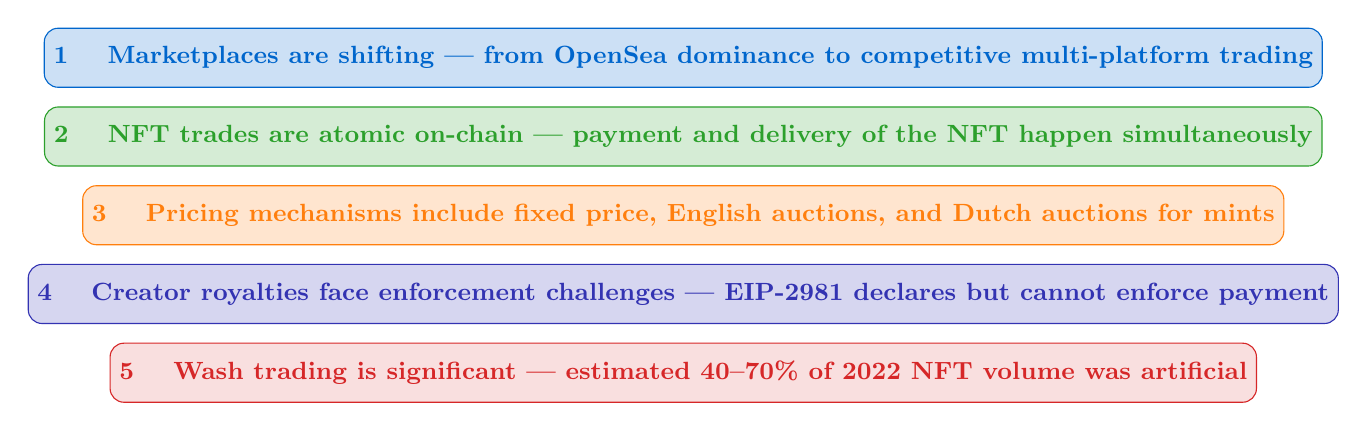
\begin{tikzpicture}[remember picture]
  \node[draw=mlblue, fill=mlblue!20, rounded corners=5pt, minimum width=11.6cm, minimum height=0.75cm, font=\small\bfseries, align=center, text=mlblue] at (6.0,5.2) {1 \quad Marketplaces are shifting --- from OpenSea dominance to competitive multi-platform trading};
  \node[draw=mlgreen, fill=mlgreen!20, rounded corners=5pt, minimum width=11.6cm, minimum height=0.75cm, font=\small\bfseries, align=center, text=mlgreen] at (6.0,4.2) {2 \quad NFT trades are atomic on-chain --- payment and delivery of the NFT happen simultaneously};
  \node[draw=mlorange, fill=mlorange!20, rounded corners=5pt, minimum width=11.6cm, minimum height=0.75cm, font=\small\bfseries, align=center, text=mlorange] at (6.0,3.2) {3 \quad Pricing mechanisms include fixed price, English auctions, and Dutch auctions for mints};
  \node[draw=mlpurple, fill=mlpurple!20, rounded corners=5pt, minimum width=11.6cm, minimum height=0.75cm, font=\small\bfseries, align=center, text=mlpurple] at (6.0,2.2) {4 \quad Creator royalties face enforcement challenges --- EIP-2981 declares but cannot enforce payment};
  \node[draw=mlred, fill=mlred!15, rounded corners=5pt, minimum width=11.6cm, minimum height=0.75cm, font=\small\bfseries, align=center, text=mlred] at (6.0,1.2) {5 \quad Wash trading is significant --- estimated 40--70\% of 2022 NFT volume was artificial};
\end{tikzpicture}
\bottomnote{Section 2 complete -- next: NFT Applications \& Use Cases}
\end{frame}

%% ============================================================
%% SECTION 3: NFT APPLICATIONS & USE CASES
%% ============================================================
\section{NFT Applications \& Use Cases}

% Frame 27: Section 3 Divider
\begin{frame}{Section 3: NFT Applications \& Use Cases}
\begin{beamercolorbox}[sep=12pt,center,rounded=true,shadow=true]{palette quaternary}
  {\Large\bfseries Section 3: NFT Applications \& Use Cases}\\[4pt]
  {\normalsize Art, gaming, music, real-world assets, identity, and credentials}
\end{beamercolorbox}

\vspace{4mm}
\begin{columns}[T]
\column{0.55\textwidth}
\begin{block}{What You Will Learn}
\begin{itemize}\setlength{\itemsep}{2pt}
  \item How digital art NFTs created verifiable scarcity for creators
  \item PFP collection mechanics and rarity distribution
  \item Gaming and play-to-earn ecosystems
  \item Music, media, and real-world asset tokenization
  \item Identity, credentials, domain names, and IP licensing
\end{itemize}
\end{block}
\column{0.42\textwidth}
\begin{block}{Frames in This Section}
\begin{itemize}\setlength{\itemsep}{1pt}
  \item Frame 27 --- Section overview
  \item Frame 28 --- Digital art NFTs
  \item Frame 29 --- PFP collections
  \item Frame 30 --- Generative art
  \item Frame 31 --- Gaming NFTs
  \item Frame 32 --- Music and media
  \item Frame 33 --- Real-world assets
  \item Frame 34 --- Identity \& credentials
  \item Frame 35 --- Domain names
  \item Frame 36 --- NFT ticketing
  \item Frame 37 --- IP and licensing
  \item Frame 38 --- Section 3 summary
\end{itemize}
\end{block}
\end{columns}
\bottomnote{Section 3 | Frames 27--38 | NFT Applications \& Use Cases}
\end{frame}

% Frame 28: Digital Art NFTs
\begin{frame}{Digital Art NFTs}
\begin{columns}[T]
\column{0.47\textwidth}
\begin{block}{Key Milestones}
\begin{itemize}\setlength{\itemsep}{3pt}
  \item \textbf{Beeple \$69M at Christie's (2021)} --- ``Everydays: The First 5000 Days'' sold as a single NFT, legitimising digital art in traditional auction houses
  \item \textbf{CryptoPunks (2017)} --- 10,000 pixelated characters; first collectible NFT project on Ethereum; free to claim at launch
  \item \textbf{Art Blocks (2020)} --- Generative art platform; each piece minted on demand from an algorithm stored on-chain
\end{itemize}
\end{block}
\vspace{2mm}
\begin{block}{Why Digital Art NFTs Matter}
Verifiable scarcity on a public ledger converts infinitely-copyable files into provably unique digital assets with traceable provenance.
\end{block}

\column{0.50\textwidth}
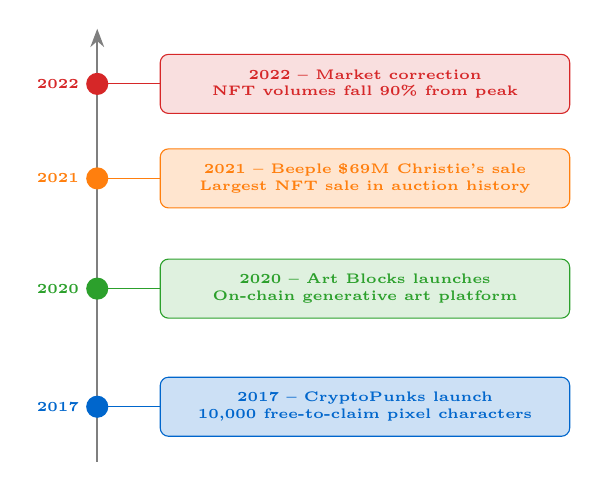
\begin{tikzpicture}[remember picture]
  % Timeline axis
  \draw[thick, mlgray] (0.5,0.3) -- (0.5,5.5);
  \draw[-{Stealth}, thick, mlgray] (0.5,5.5) -- (0.5,5.8);

  % 2017 - CryptoPunks
  \fill[mlblue] (0.5,1.0) circle (4pt);
  \draw[mlblue, thin] (0.5,1.0) -- (1.3,1.0);
  \node[draw=mlblue, fill=mlblue!20, rounded corners=3pt, minimum width=5.2cm, minimum height=0.75cm, font=\tiny\bfseries, align=center, text=mlblue] at (3.9,1.0) {2017 -- CryptoPunks launch\\10,000 free-to-claim pixel characters};

  % 2020 - Art Blocks
  \fill[mlgreen] (0.5,2.5) circle (4pt);
  \draw[mlgreen, thin] (0.5,2.5) -- (1.3,2.5);
  \node[draw=mlgreen, fill=mlgreen!15, rounded corners=3pt, minimum width=5.2cm, minimum height=0.75cm, font=\tiny\bfseries, align=center, text=mlgreen] at (3.9,2.5) {2020 -- Art Blocks launches\\On-chain generative art platform};

  % 2021 - Beeple record
  \fill[mlorange] (0.5,3.9) circle (4pt);
  \draw[mlorange, thin] (0.5,3.9) -- (1.3,3.9);
  \node[draw=mlorange, fill=mlorange!20, rounded corners=3pt, minimum width=5.2cm, minimum height=0.75cm, font=\tiny\bfseries, align=center, text=mlorange] at (3.9,3.9) {2021 -- Beeple \$69M Christie's sale\\Largest NFT sale in auction history};

  % 2022 - correction
  \fill[mlred] (0.5,5.1) circle (4pt);
  \draw[mlred, thin] (0.5,5.1) -- (1.3,5.1);
  \node[draw=mlred, fill=mlred!15, rounded corners=3pt, minimum width=5.2cm, minimum height=0.75cm, font=\tiny\bfseries, align=center, text=mlred] at (3.9,5.1) {2022 -- Market correction\\NFT volumes fall 90\% from peak};

  % Year labels on axis
  \node[font=\tiny\bfseries, text=mlblue] at (0.0,1.0) {2017};
  \node[font=\tiny\bfseries, text=mlgreen] at (0.0,2.5) {2020};
  \node[font=\tiny\bfseries, text=mlorange] at (0.0,3.9) {2021};
  \node[font=\tiny\bfseries, text=mlred] at (0.0,5.1) {2022};
\end{tikzpicture}
\end{columns}
\bottomnote{Digital art NFTs proved that verifiable scarcity can create real value for digital creators}
\end{frame}

% Frame 29: Profile Picture (PFP) Collections
\begin{frame}{Profile Picture (PFP) Collections}
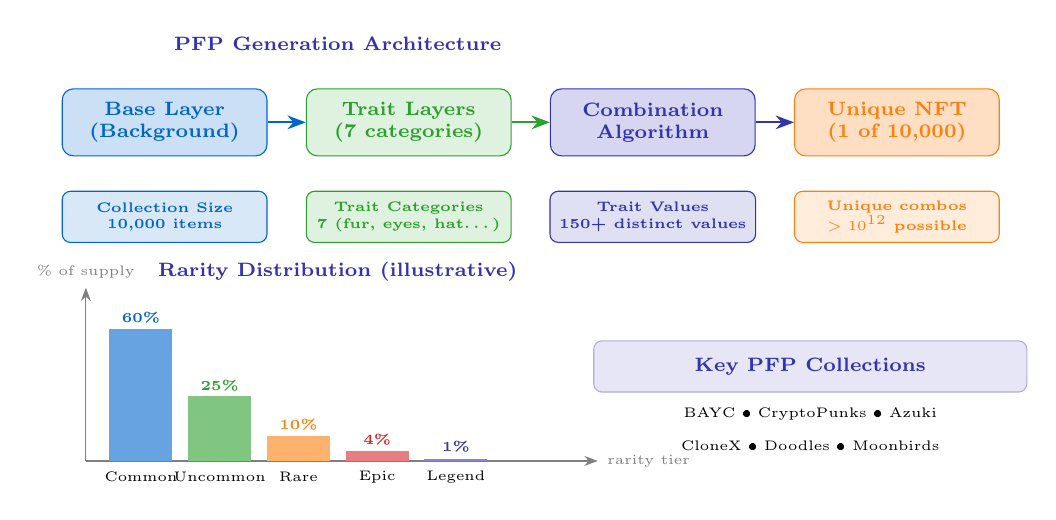
\begin{tikzpicture}[remember picture]
  %--- Generation pipeline ---
  \node[font=\scriptsize\bfseries, text=mlpurple] at (3.5,5.6) {PFP Generation Architecture};

  % Base layer box
  \node[draw=mlblue, fill=mlblue!20, rounded corners=4pt, minimum width=2.6cm, minimum height=0.85cm, font=\scriptsize\bfseries, align=center, text=mlblue] (base) at (1.3,4.6) {Base Layer\\(Background)};
  % Trait layers
  \node[draw=mlgreen, fill=mlgreen!15, rounded corners=4pt, minimum width=2.6cm, minimum height=0.85cm, font=\scriptsize\bfseries, align=center, text=mlgreen] (traits) at (4.4,4.6) {Trait Layers\\(7 categories)};
  % Algorithm
  \node[draw=mlpurple, fill=mlpurple!20, rounded corners=4pt, minimum width=2.6cm, minimum height=0.85cm, font=\scriptsize\bfseries, align=center, text=mlpurple] (algo) at (7.5,4.6) {Combination\\Algorithm};
  % Unique NFT
  \node[draw=mlorange, fill=mlorange!25, rounded corners=4pt, minimum width=2.6cm, minimum height=0.85cm, font=\scriptsize\bfseries, align=center, text=mlorange] (nft) at (10.6,4.6) {Unique NFT\\(1 of 10,000)};

  \draw[-{Stealth}, thick, mlblue] (base.east) -- (traits.west);
  \draw[-{Stealth}, thick, mlgreen] (traits.east) -- (algo.west);
  \draw[-{Stealth}, thick, mlpurple] (algo.east) -- (nft.west);

  %--- Stats row ---
  \node[draw=mlblue, fill=mlblue!15, rounded corners=3pt, minimum width=2.6cm, minimum height=0.65cm, font=\tiny\bfseries, align=center, text=mlblue] at (1.3,3.4) {Collection Size\\10,000 items};
  \node[draw=mlgreen, fill=mlgreen!15, rounded corners=3pt, minimum width=2.6cm, minimum height=0.65cm, font=\tiny\bfseries, align=center, text=mlgreen] at (4.4,3.4) {Trait Categories\\7 (fur, eyes, hat\ldots)};
  \node[draw=mlpurple, fill=mlpurple!15, rounded corners=3pt, minimum width=2.6cm, minimum height=0.65cm, font=\tiny\bfseries, align=center, text=mlpurple] at (7.5,3.4) {Trait Values\\150+ distinct values};
  \node[draw=mlorange, fill=mlorange!15, rounded corners=3pt, minimum width=2.6cm, minimum height=0.65cm, font=\tiny\bfseries, align=center, text=mlorange] at (10.6,3.4) {Unique combos\\$> 10^{12}$ possible};

  %--- Rarity bar chart (manual bars) ---
  \node[font=\scriptsize\bfseries, text=mlpurple] at (3.5,2.7) {Rarity Distribution (illustrative)};

  % Axes
  \draw[-{Stealth}, thin, mlgray] (0.3,0.3) -- (6.8,0.3) node[right, font=\tiny] {rarity tier};
  \draw[-{Stealth}, thin, mlgray] (0.3,0.3) -- (0.3,2.5) node[above, font=\tiny] {\% of supply};

  % Bars (Common 60%, Uncommon 25%, Rare 10%, Epic 4%, Legendary 1%)
  \fill[mlblue!60] (0.6,0.3) rectangle (1.4,1.98);
  \fill[mlgreen!60] (1.6,0.3) rectangle (2.4,1.125);
  \fill[mlorange!60] (2.6,0.3) rectangle (3.4,0.615);
  \fill[mlred!60] (3.6,0.3) rectangle (4.4,0.42);
  \fill[mlpurple!60] (4.6,0.3) rectangle (5.4,0.33);

  % Bar labels (values)
  \node[font=\tiny\bfseries, text=mlblue] at (1.0,2.12) {60\%};
  \node[font=\tiny\bfseries, text=mlgreen] at (2.0,1.25) {25\%};
  \node[font=\tiny\bfseries, text=mlorange] at (3.0,0.76) {10\%};
  \node[font=\tiny\bfseries, text=mlred] at (4.0,0.57) {4\%};
  \node[font=\tiny\bfseries, text=mlpurple] at (5.0,0.48) {1\%};

  % X-axis labels
  \node[font=\tiny] at (1.0,0.1) {Common};
  \node[font=\tiny] at (2.0,0.1) {Uncommon};
  \node[font=\tiny] at (3.0,0.1) {Rare};
  \node[font=\tiny] at (4.0,0.1) {Epic};
  \node[font=\tiny] at (5.0,0.1) {Legend};

  %--- Key collections ---
  \node[draw=mllavender, fill=mllavender!30, rounded corners=3pt, minimum width=5.5cm, minimum height=0.65cm, font=\scriptsize\bfseries, align=center, text=mlpurple] at (9.5,1.5) {Key PFP Collections};
  \node[font=\tiny, align=center] at (9.5,0.9) {BAYC \textbullet{} CryptoPunks \textbullet{} Azuki};
  \node[font=\tiny, align=center] at (9.5,0.5) {CloneX \textbullet{} Doodles \textbullet{} Moonbirds};
\end{tikzpicture}
\bottomnote{PFP collections use algorithmic generation to create thousands of unique but thematically consistent NFTs}
\end{frame}

% Frame 30: Generative Art NFTs
\begin{frame}{Generative Art NFTs}
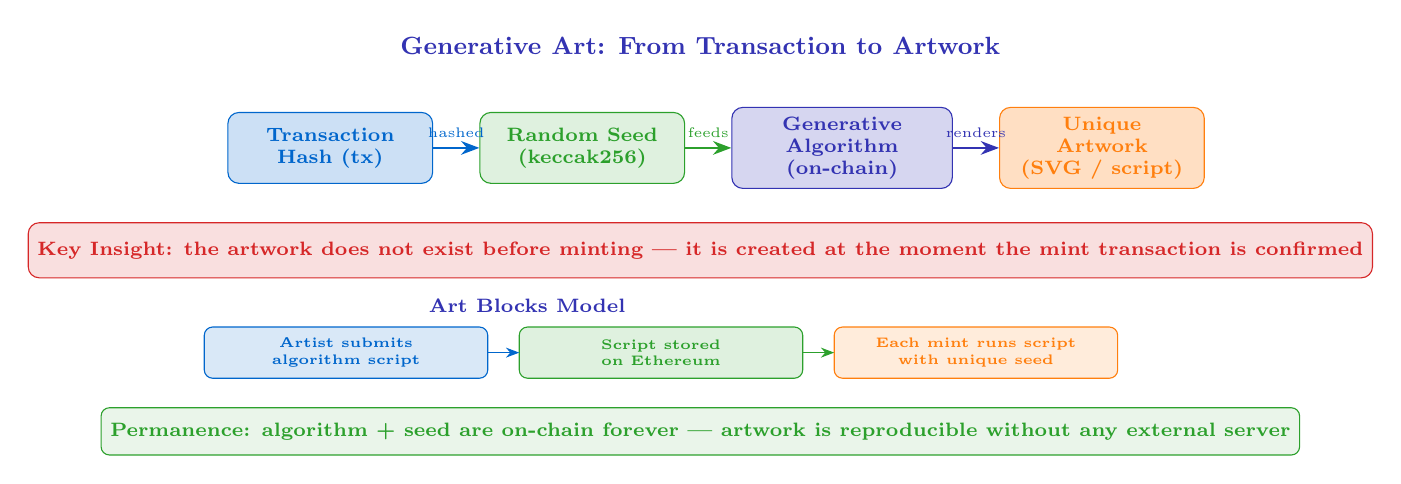
\begin{tikzpicture}[remember picture]
  %--- Main pipeline ---
  \node[font=\small\bfseries, text=mlpurple] at (6.0,5.6) {Generative Art: From Transaction to Artwork};

  % Transaction hash
  \node[draw=mlblue, fill=mlblue!20, rounded corners=4pt, minimum width=2.6cm, minimum height=0.9cm, font=\scriptsize\bfseries, align=center, text=mlblue] (txhash) at (1.3,4.3) {Transaction\\Hash (tx)};

  % Random seed
  \node[draw=mlgreen, fill=mlgreen!15, rounded corners=4pt, minimum width=2.6cm, minimum height=0.9cm, font=\scriptsize\bfseries, align=center, text=mlgreen] (seed) at (4.5,4.3) {Random Seed\\(keccak256)};

  % Generative algorithm
  \node[draw=mlpurple, fill=mlpurple!20, rounded corners=4pt, minimum width=2.8cm, minimum height=0.9cm, font=\scriptsize\bfseries, align=center, text=mlpurple] (algo) at (7.8,4.3) {Generative\\Algorithm\\(on-chain)};

  % Unique artwork
  \node[draw=mlorange, fill=mlorange!25, rounded corners=4pt, minimum width=2.6cm, minimum height=0.9cm, font=\scriptsize\bfseries, align=center, text=mlorange] (art) at (11.1,4.3) {Unique\\Artwork\\(SVG / script)};

  \draw[-{Stealth}, thick, mlblue] (txhash.east) -- node[above, font=\tiny] {hashed} (seed.west);
  \draw[-{Stealth}, thick, mlgreen] (seed.east) -- node[above, font=\tiny] {feeds} (algo.west);
  \draw[-{Stealth}, thick, mlpurple] (algo.east) -- node[above, font=\tiny] {renders} (art.west);

  %--- Key insight box ---
  \node[draw=mlred, fill=mlred!15, rounded corners=4pt, minimum width=11.5cm, minimum height=0.7cm, font=\scriptsize\bfseries, align=center, text=mlred] at (6.0,3.0) {Key Insight: the artwork does not exist before minting --- it is created at the moment the mint transaction is confirmed};

  %--- Art Blocks model ---
  \node[font=\scriptsize\bfseries, text=mlpurple] at (3.8,2.3) {Art Blocks Model};

  \node[draw=mlblue, fill=mlblue!15, rounded corners=3pt, minimum width=3.6cm, minimum height=0.65cm, font=\tiny\bfseries, align=center, text=mlblue] at (1.5,1.7) {Artist submits\\algorithm script};
  \node[draw=mlgreen, fill=mlgreen!15, rounded corners=3pt, minimum width=3.6cm, minimum height=0.65cm, font=\tiny\bfseries, align=center, text=mlgreen] at (5.5,1.7) {Script stored\\on Ethereum};
  \node[draw=mlorange, fill=mlorange!15, rounded corners=3pt, minimum width=3.6cm, minimum height=0.65cm, font=\tiny\bfseries, align=center, text=mlorange] at (9.5,1.7) {Each mint runs script\\with unique seed};

  \draw[-{Stealth}, thin, mlblue] (3.3,1.7) -- (3.7,1.7);
  \draw[-{Stealth}, thin, mlgreen] (7.3,1.7) -- (7.7,1.7);

  %--- Permanence note ---
  \node[draw=mlgreen, fill=mlgreen!10, rounded corners=3pt, minimum width=11.5cm, minimum height=0.6cm, font=\scriptsize\bfseries, align=center, text=mlgreen] at (6.0,0.7) {Permanence: algorithm + seed are on-chain forever --- artwork is reproducible without any external server};
\end{tikzpicture}
\bottomnote{Generative art NFTs are unique because the artwork is created on-chain at the moment of minting}
\end{frame}

% Frame 31: Gaming NFTs
\begin{frame}{Gaming NFTs}
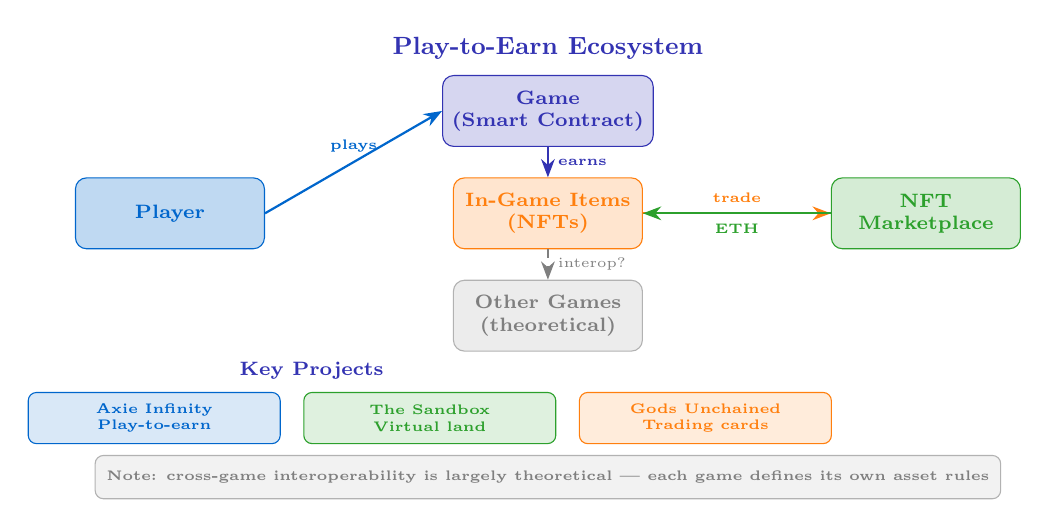
\begin{tikzpicture}[remember picture]
  %--- Ecosystem diagram ---
  \node[font=\small\bfseries, text=mlpurple] at (6.0,5.6) {Play-to-Earn Ecosystem};

  % Player node
  \node[draw=mlblue, fill=mlblue!25, rounded corners=4pt, minimum width=2.4cm, minimum height=0.9cm, font=\scriptsize\bfseries, align=center, text=mlblue] (player) at (1.2,3.5) {Player};

  % Game node
  \node[draw=mlpurple, fill=mlpurple!20, rounded corners=4pt, minimum width=2.4cm, minimum height=0.9cm, font=\scriptsize\bfseries, align=center, text=mlpurple] (game) at (6.0,4.8) {Game\\(Smart Contract)};

  % NFT items node
  \node[draw=mlorange, fill=mlorange!20, rounded corners=4pt, minimum width=2.4cm, minimum height=0.9cm, font=\scriptsize\bfseries, align=center, text=mlorange] (items) at (6.0,3.5) {In-Game Items\\(NFTs)};

  % Marketplace node
  \node[draw=mlgreen, fill=mlgreen!20, rounded corners=4pt, minimum width=2.4cm, minimum height=0.9cm, font=\scriptsize\bfseries, align=center, text=mlgreen] (market) at (10.8,3.5) {NFT\\Marketplace};

  % Theoretical interop node
  \node[draw=mlgray!60, fill=mlgray!15, rounded corners=4pt, minimum width=2.4cm, minimum height=0.9cm, font=\scriptsize\bfseries, align=center, text=mlgray] (interop) at (6.0,2.2) {Other Games\\(theoretical)};

  % Arrows
  \draw[-{Stealth}, thick, mlblue] (player.east) -- node[above, font=\tiny\bfseries] {plays} (game.west);
  \draw[-{Stealth}, thick, mlpurple] (game.south) -- node[right, font=\tiny\bfseries] {earns} (items.north);
  \draw[-{Stealth}, thick, mlorange] (items.east) -- node[above, font=\tiny\bfseries] {trade} (market.west);
  \draw[-{Stealth}, thick, mlgreen] (market.west) -- node[below, font=\tiny\bfseries] {ETH} (items.east);
  \draw[-{Stealth}, thick, mlgray, dashed] (items.south) -- node[right, font=\tiny, text=mlgray] {interop?} (interop.north);

  %--- Examples ---
  \node[font=\scriptsize\bfseries, text=mlpurple] at (3.0,1.5) {Key Projects};

  \node[draw=mlblue, fill=mlblue!15, rounded corners=3pt, minimum width=3.2cm, minimum height=0.65cm, font=\tiny\bfseries, align=center, text=mlblue] at (1.0,0.9) {Axie Infinity\\Play-to-earn};
  \node[draw=mlgreen, fill=mlgreen!15, rounded corners=3pt, minimum width=3.2cm, minimum height=0.65cm, font=\tiny\bfseries, align=center, text=mlgreen] at (4.5,0.9) {The Sandbox\\Virtual land};
  \node[draw=mlorange, fill=mlorange!15, rounded corners=3pt, minimum width=3.2cm, minimum height=0.65cm, font=\tiny\bfseries, align=center, text=mlorange] at (8.0,0.9) {Gods Unchained\\Trading cards};

  % Caveat
  \node[draw=mlgray!60, fill=mlgray!10, rounded corners=3pt, minimum width=11.5cm, minimum height=0.55cm, font=\tiny\bfseries, align=center, text=mlgray] at (6.0,0.15) {Note: cross-game interoperability is largely theoretical --- each game defines its own asset rules};
\end{tikzpicture}
\bottomnote{Gaming NFTs give players true ownership of in-game assets -- but interoperability remains largely theoretical}
\end{frame}

% Frame 32: Music and Media NFTs
\begin{frame}{Music and Media NFTs}
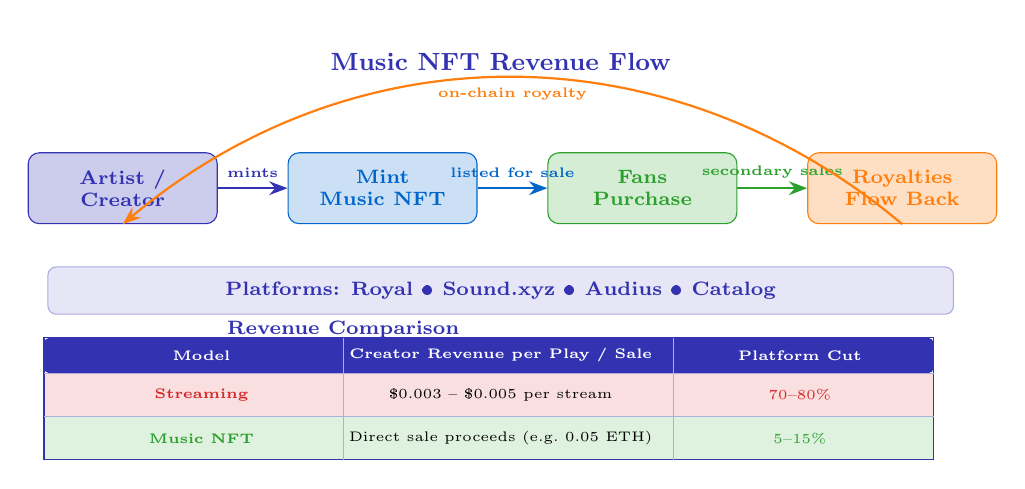
\begin{tikzpicture}[remember picture]
  %--- Revenue flow ---
  \node[font=\small\bfseries, text=mlpurple] at (6.0,5.6) {Music NFT Revenue Flow};

  % Creator
  \node[draw=mlpurple, fill=mlpurple!25, rounded corners=4pt, minimum width=2.4cm, minimum height=0.9cm, font=\scriptsize\bfseries, align=center, text=mlpurple] (creator) at (1.2,4.0) {Artist /\\Creator};

  % Mint NFT
  \node[draw=mlblue, fill=mlblue!20, rounded corners=4pt, minimum width=2.4cm, minimum height=0.9cm, font=\scriptsize\bfseries, align=center, text=mlblue] (mint) at (4.5,4.0) {Mint\\Music NFT};

  % Fans
  \node[draw=mlgreen, fill=mlgreen!20, rounded corners=4pt, minimum width=2.4cm, minimum height=0.9cm, font=\scriptsize\bfseries, align=center, text=mlgreen] (fans) at (7.8,4.0) {Fans\\Purchase};

  % Royalties
  \node[draw=mlorange, fill=mlorange!25, rounded corners=4pt, minimum width=2.4cm, minimum height=0.9cm, font=\scriptsize\bfseries, align=center, text=mlorange] (royalty) at (11.1,4.0) {Royalties\\Flow Back};

  \draw[-{Stealth}, thick, mlpurple] (creator.east) -- node[above, font=\tiny\bfseries] {mints} (mint.west);
  \draw[-{Stealth}, thick, mlblue] (mint.east) -- node[above, font=\tiny\bfseries] {listed for sale} (fans.west);
  \draw[-{Stealth}, thick, mlgreen] (fans.east) -- node[above, font=\tiny\bfseries] {secondary sales} (royalty.west);
  \draw[-{Stealth}, thick, mlorange, bend right=40] (royalty.south) to node[below, font=\tiny\bfseries] {on-chain royalty} (creator.south);

  %--- Platforms ---
  \node[draw=mllavender, fill=mllavender!30, rounded corners=3pt, minimum width=11.5cm, minimum height=0.6cm, font=\scriptsize\bfseries, align=center, text=mlpurple] at (6.0,2.7) {Platforms: Royal \textbullet{} Sound.xyz \textbullet{} Audius \textbullet{} Catalog};

  %--- Comparison table ---
  \node[font=\scriptsize\bfseries, text=mlpurple] at (4.0,2.2) {Revenue Comparison};

  % Header
  \fill[mlpurple, rounded corners=2pt] (0.2,1.65) rectangle (11.5,2.1);
  \node[font=\tiny\bfseries, text=white] at (2.2,1.875) {Model};
  \node[font=\tiny\bfseries, text=white] at (6.0,1.875) {Creator Revenue per Play / Sale};
  \node[font=\tiny\bfseries, text=white] at (9.8,1.875) {Platform Cut};

  % Row 1: Streaming
  \fill[mlred!15] (0.2,1.1) rectangle (11.5,1.65);
  \node[font=\tiny\bfseries, text=mlred] at (2.2,1.375) {Streaming};
  \node[font=\tiny] at (6.0,1.375) {\$0.003 -- \$0.005 per stream};
  \node[font=\tiny, text=mlred] at (9.8,1.375) {70--80\%};

  % Row 2: Music NFT
  \fill[mlgreen!15] (0.2,0.55) rectangle (11.5,1.1);
  \node[font=\tiny\bfseries, text=mlgreen] at (2.2,0.825) {Music NFT};
  \node[font=\tiny] at (6.0,0.825) {Direct sale proceeds (e.g.\ 0.05 ETH)};
  \node[font=\tiny, text=mlgreen] at (9.8,0.825) {5--15\%};

  % Border
  \draw[mlpurple, thin] (0.2,0.55) rectangle (11.5,2.1);
  \draw[mlpurple!40, thin] (4.0,0.55) -- (4.0,2.1);
  \draw[mlpurple!40, thin] (8.2,0.55) -- (8.2,2.1);
  \draw[mlpurple!40, thin] (0.2,1.1) -- (11.5,1.1);
  \draw[mlpurple!40, thin] (0.2,1.65) -- (11.5,1.65);
\end{tikzpicture}
\bottomnote{Music NFTs let artists earn directly from fans without intermediary platforms taking 70--80\% of revenue}
\end{frame}

% Frame 33: Real-World Asset (RWA) Tokenization
\begin{frame}{Real-World Asset (RWA) Tokenization}
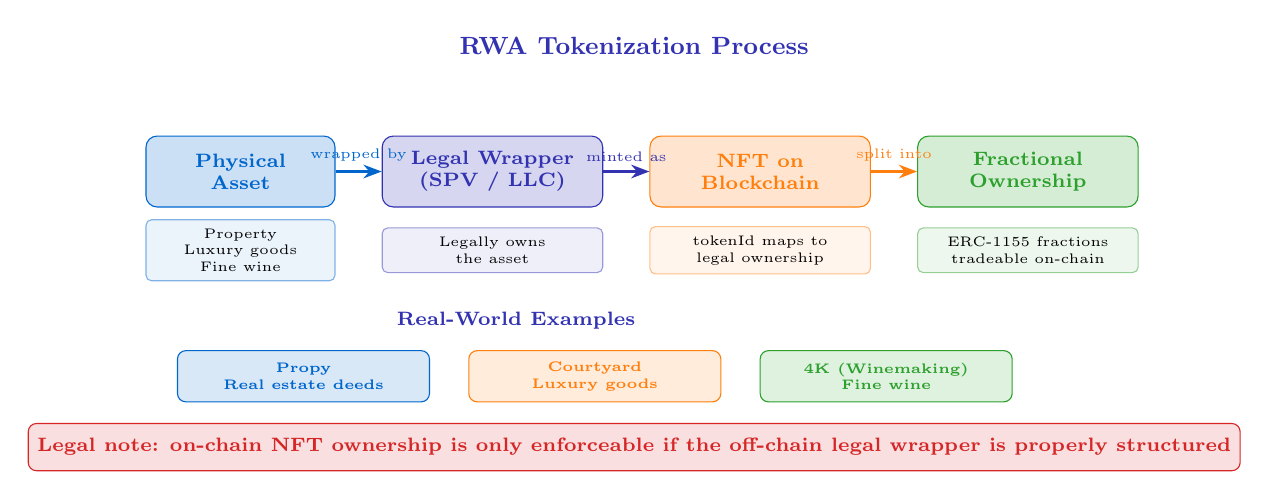
\begin{tikzpicture}[remember picture]
  \node[font=\small\bfseries, text=mlpurple] at (6.0,5.6) {RWA Tokenization Process};

  % Step 1: Physical asset
  \node[draw=mlblue, fill=mlblue!20, rounded corners=4pt, minimum width=2.4cm, minimum height=0.9cm, font=\scriptsize\bfseries, align=center, text=mlblue] (asset) at (1.0,4.0) {Physical\\Asset};

  % Step 2: Legal wrapper
  \node[draw=mlpurple, fill=mlpurple!20, rounded corners=4pt, minimum width=2.8cm, minimum height=0.9cm, font=\scriptsize\bfseries, align=center, text=mlpurple] (legal) at (4.2,4.0) {Legal Wrapper\\(SPV / LLC)};

  % Step 3: NFT on-chain
  \node[draw=mlorange, fill=mlorange!20, rounded corners=4pt, minimum width=2.8cm, minimum height=0.9cm, font=\scriptsize\bfseries, align=center, text=mlorange] (nft) at (7.6,4.0) {NFT on\\Blockchain};

  % Step 4: Fractional ownership
  \node[draw=mlgreen, fill=mlgreen!20, rounded corners=4pt, minimum width=2.8cm, minimum height=0.9cm, font=\scriptsize\bfseries, align=center, text=mlgreen] (frac) at (11.0,4.0) {Fractional\\Ownership};

  \draw[-{Stealth}, thick, mlblue] (asset.east) -- node[above, font=\tiny] {wrapped by} (legal.west);
  \draw[-{Stealth}, thick, mlpurple] (legal.east) -- node[above, font=\tiny] {minted as} (nft.west);
  \draw[-{Stealth}, thick, mlorange] (nft.east) -- node[above, font=\tiny] {split into} (frac.west);

  %--- Sub-labels ---
  \node[draw=mlblue!50, fill=mlblue!8, rounded corners=2pt, minimum width=2.4cm, minimum height=0.55cm, font=\tiny, align=center] at (1.0,3.0) {Property\\Luxury goods\\Fine wine};
  \node[draw=mlpurple!50, fill=mlpurple!8, rounded corners=2pt, minimum width=2.8cm, minimum height=0.55cm, font=\tiny, align=center] at (4.2,3.0) {Legally owns\\the asset};
  \node[draw=mlorange!50, fill=mlorange!8, rounded corners=2pt, minimum width=2.8cm, minimum height=0.55cm, font=\tiny, align=center] at (7.6,3.0) {tokenId maps to\\legal ownership};
  \node[draw=mlgreen!50, fill=mlgreen!8, rounded corners=2pt, minimum width=2.8cm, minimum height=0.55cm, font=\tiny, align=center] at (11.0,3.0) {ERC-1155 fractions\\tradeable on-chain};

  %--- Examples ---
  \node[font=\scriptsize\bfseries, text=mlpurple] at (4.5,2.1) {Real-World Examples};

  \node[draw=mlblue, fill=mlblue!15, rounded corners=3pt, minimum width=3.2cm, minimum height=0.65cm, font=\tiny\bfseries, align=center, text=mlblue] at (1.8,1.4) {Propy\\Real estate deeds};
  \node[draw=mlorange, fill=mlorange!15, rounded corners=3pt, minimum width=3.2cm, minimum height=0.65cm, font=\tiny\bfseries, align=center, text=mlorange] at (5.5,1.4) {Courtyard\\Luxury goods};
  \node[draw=mlgreen, fill=mlgreen!15, rounded corners=3pt, minimum width=3.2cm, minimum height=0.65cm, font=\tiny\bfseries, align=center, text=mlgreen] at (9.2,1.4) {4K (Winemaking)\\Fine wine};

  %--- Legal note ---
  \node[draw=mlred, fill=mlred!15, rounded corners=3pt, minimum width=11.5cm, minimum height=0.6cm, font=\scriptsize\bfseries, align=center, text=mlred] at (6.0,0.5) {Legal note: on-chain NFT ownership is only enforceable if the off-chain legal wrapper is properly structured};
\end{tikzpicture}
\bottomnote{RWA tokenization bridges physical and digital ownership -- legal frameworks are still evolving}
\end{frame}

% Frame 34: Identity and Credential NFTs
\begin{frame}{Identity and Credential NFTs}
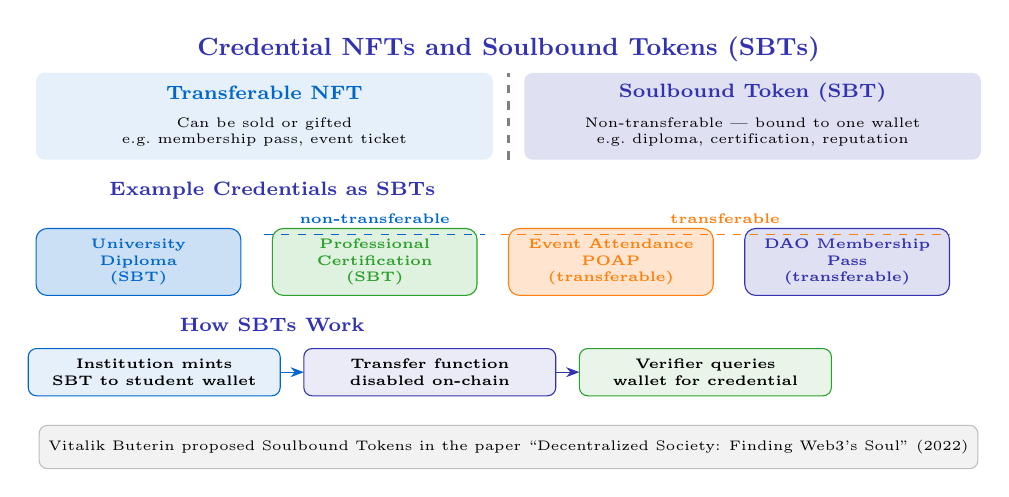
\begin{tikzpicture}[remember picture]
  \node[font=\small\bfseries, text=mlpurple] at (6.0,5.6) {Credential NFTs and Soulbound Tokens (SBTs)};

  %--- Transferable vs Soulbound ---
  \fill[mlblue!10, rounded corners=3pt] (0.0,4.2) rectangle (5.8,5.3);
  \node[font=\scriptsize\bfseries, text=mlblue] at (2.9,5.05) {Transferable NFT};
  \node[font=\tiny, align=center] at (2.9,4.55) {Can be sold or gifted\\e.g.\ membership pass, event ticket};

  \fill[mlpurple!15, rounded corners=3pt] (6.2,4.2) rectangle (12.0,5.3);
  \node[font=\scriptsize\bfseries, text=mlpurple] at (9.1,5.05) {Soulbound Token (SBT)};
  \node[font=\tiny, align=center] at (9.1,4.55) {Non-transferable --- bound to one wallet\\e.g.\ diploma, certification, reputation};

  \draw[thick, mlgray, dashed] (6.0,4.2) -- (6.0,5.3);

  %--- Example credential cards ---
  \node[font=\scriptsize\bfseries, text=mlpurple] at (3.0,3.8) {Example Credentials as SBTs};

  % Diploma
  \node[draw=mlblue, fill=mlblue!20, rounded corners=4pt, minimum width=2.6cm, minimum height=0.85cm, font=\tiny\bfseries, align=center, text=mlblue] (dip) at (1.3,2.9) {University\\Diploma\\(SBT)};

  % Professional cert
  \node[draw=mlgreen, fill=mlgreen!15, rounded corners=4pt, minimum width=2.6cm, minimum height=0.85cm, font=\tiny\bfseries, align=center, text=mlgreen] (cert) at (4.3,2.9) {Professional\\Certification\\(SBT)};

  % POAP
  \node[draw=mlorange, fill=mlorange!20, rounded corners=4pt, minimum width=2.6cm, minimum height=0.85cm, font=\tiny\bfseries, align=center, text=mlorange] (poap) at (7.3,2.9) {Event Attendance\\POAP\\(transferable)};

  % Membership
  \node[draw=mlpurple, fill=mlpurple!15, rounded corners=4pt, minimum width=2.6cm, minimum height=0.85cm, font=\tiny\bfseries, align=center, text=mlpurple] (mem) at (10.3,2.9) {DAO Membership\\Pass\\(transferable)};

  % Connecting line
  \draw[mlblue, thin, dashed] (2.9,3.25) -- (5.7,3.25);
  \node[font=\tiny\bfseries, text=mlblue] at (4.3,3.45) {non-transferable};
  \draw[mlorange, thin, dashed] (5.9,3.25) -- (11.6,3.25);
  \node[font=\tiny\bfseries, text=mlorange] at (8.75,3.45) {transferable};

  %--- How it works ---
  \node[font=\scriptsize\bfseries, text=mlpurple] at (3.0,2.1) {How SBTs Work};

  \node[draw=mlblue, fill=mlblue!10, rounded corners=3pt, minimum width=3.2cm, minimum height=0.6cm, font=\tiny\bfseries, align=center] at (1.5,1.5) {Institution mints\\SBT to student wallet};
  \node[draw=mlpurple, fill=mlpurple!10, rounded corners=3pt, minimum width=3.2cm, minimum height=0.6cm, font=\tiny\bfseries, align=center] at (5.0,1.5) {Transfer function\\disabled on-chain};
  \node[draw=mlgreen, fill=mlgreen!10, rounded corners=3pt, minimum width=3.2cm, minimum height=0.6cm, font=\tiny\bfseries, align=center] at (8.5,1.5) {Verifier queries\\wallet for credential};

  \draw[-{Stealth}, thin, mlblue] (3.1,1.5) -- (3.4,1.5);
  \draw[-{Stealth}, thin, mlpurple] (6.6,1.5) -- (6.9,1.5);

  \node[draw=mlgray!50, fill=mlgray!10, rounded corners=3pt, minimum width=11.5cm, minimum height=0.55cm, font=\tiny, align=center] at (6.0,0.55) {Vitalik Buterin proposed Soulbound Tokens in the paper ``Decentralized Society: Finding Web3's Soul'' (2022)};
\end{tikzpicture}
\bottomnote{Credential NFTs and soulbound tokens may replace traditional paper certificates and membership cards}
\end{frame}

% Frame 35: Domain Names as NFTs
\begin{frame}{Domain Names as NFTs}
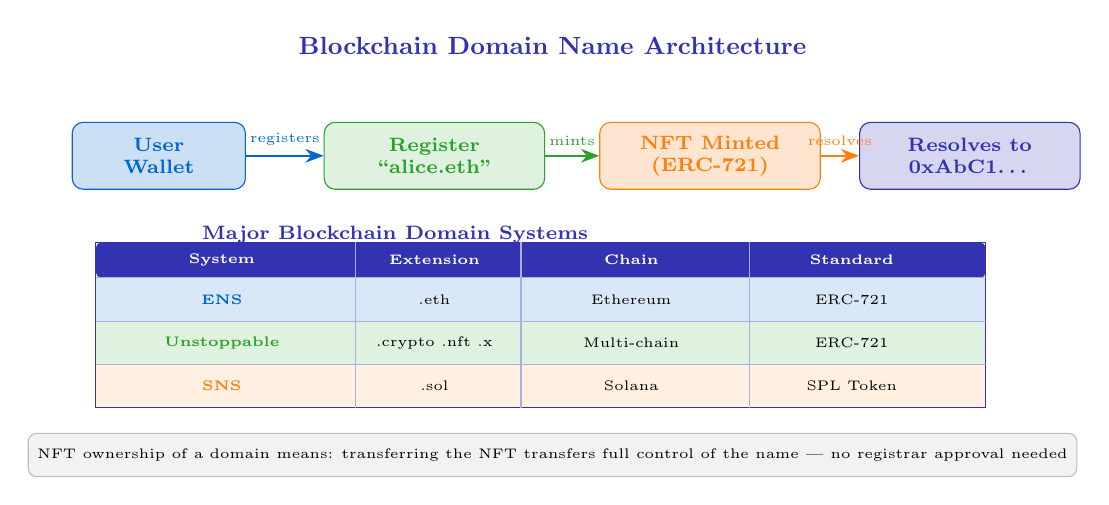
\begin{tikzpicture}[remember picture]
  \node[font=\small\bfseries, text=mlpurple] at (6.0,5.6) {Blockchain Domain Name Architecture};

  %--- Registration flow ---
  % User
  \node[draw=mlblue, fill=mlblue!20, rounded corners=4pt, minimum width=2.2cm, minimum height=0.85cm, font=\scriptsize\bfseries, align=center, text=mlblue] (user) at (1.0,4.2) {User\\Wallet};

  % Registers name
  \node[draw=mlgreen, fill=mlgreen!15, rounded corners=4pt, minimum width=2.8cm, minimum height=0.85cm, font=\scriptsize\bfseries, align=center, text=mlgreen] (reg) at (4.5,4.2) {Register\\``alice.eth''};

  % NFT minted
  \node[draw=mlorange, fill=mlorange!20, rounded corners=4pt, minimum width=2.8cm, minimum height=0.85cm, font=\scriptsize\bfseries, align=center, text=mlorange] (nft) at (8.0,4.2) {NFT Minted\\(ERC-721)};

  % Resolves to address
  \node[draw=mlpurple, fill=mlpurple!20, rounded corners=4pt, minimum width=2.8cm, minimum height=0.85cm, font=\scriptsize\bfseries, align=center, text=mlpurple] (resolve) at (11.3,4.2) {Resolves to\\0xAbC1\ldots};

  \draw[-{Stealth}, thick, mlblue] (user.east) -- node[above, font=\tiny] {registers} (reg.west);
  \draw[-{Stealth}, thick, mlgreen] (reg.east) -- node[above, font=\tiny] {mints} (nft.west);
  \draw[-{Stealth}, thick, mlorange] (nft.east) -- node[above, font=\tiny] {resolves} (resolve.west);

  %--- Comparison table ---
  \node[font=\scriptsize\bfseries, text=mlpurple] at (4.0,3.2) {Major Blockchain Domain Systems};

  % Header
  \fill[mlpurple, rounded corners=2pt] (0.2,2.65) rectangle (11.5,3.1);
  \node[font=\tiny\bfseries, text=white] at (1.8,2.875) {System};
  \node[font=\tiny\bfseries, text=white] at (4.5,2.875) {Extension};
  \node[font=\tiny\bfseries, text=white] at (7.0,2.875) {Chain};
  \node[font=\tiny\bfseries, text=white] at (9.8,2.875) {Standard};

  % Row 1: ENS
  \fill[mlblue!15] (0.2,2.1) rectangle (11.5,2.65);
  \node[font=\tiny\bfseries, text=mlblue] at (1.8,2.375) {ENS};
  \node[font=\tiny] at (4.5,2.375) {.eth};
  \node[font=\tiny] at (7.0,2.375) {Ethereum};
  \node[font=\tiny] at (9.8,2.375) {ERC-721};

  % Row 2: Unstoppable
  \fill[mlgreen!15] (0.2,1.55) rectangle (11.5,2.1);
  \node[font=\tiny\bfseries, text=mlgreen] at (1.8,1.825) {Unstoppable};
  \node[font=\tiny] at (4.5,1.825) {.crypto .nft .x};
  \node[font=\tiny] at (7.0,1.825) {Multi-chain};
  \node[font=\tiny] at (9.8,1.825) {ERC-721};

  % Row 3: SNS
  \fill[mlorange!12] (0.2,1.0) rectangle (11.5,1.55);
  \node[font=\tiny\bfseries, text=mlorange] at (1.8,1.275) {SNS};
  \node[font=\tiny] at (4.5,1.275) {.sol};
  \node[font=\tiny] at (7.0,1.275) {Solana};
  \node[font=\tiny] at (9.8,1.275) {SPL Token};

  % Border
  \draw[mlpurple, thin] (0.2,1.0) rectangle (11.5,3.1);
  \draw[mlpurple!40, thin] (3.5,1.0) -- (3.5,3.1);
  \draw[mlpurple!40, thin] (5.6,1.0) -- (5.6,3.1);
  \draw[mlpurple!40, thin] (8.5,1.0) -- (8.5,3.1);
  \draw[mlpurple!40, thin] (0.2,1.55) -- (11.5,1.55);
  \draw[mlpurple!40, thin] (0.2,2.1) -- (11.5,2.1);
  \draw[mlpurple!40, thin] (0.2,2.65) -- (11.5,2.65);

  \node[draw=mlgray!50, fill=mlgray!10, rounded corners=3pt, minimum width=11.5cm, minimum height=0.55cm, font=\tiny, align=center] at (6.0,0.4) {NFT ownership of a domain means: transferring the NFT transfers full control of the name --- no registrar approval needed};
\end{tikzpicture}
\bottomnote{Blockchain domain names are NFTs that map human-readable names to wallet addresses}
\end{frame}

% Frame 36: NFT Ticketing
\begin{frame}{NFT Ticketing}
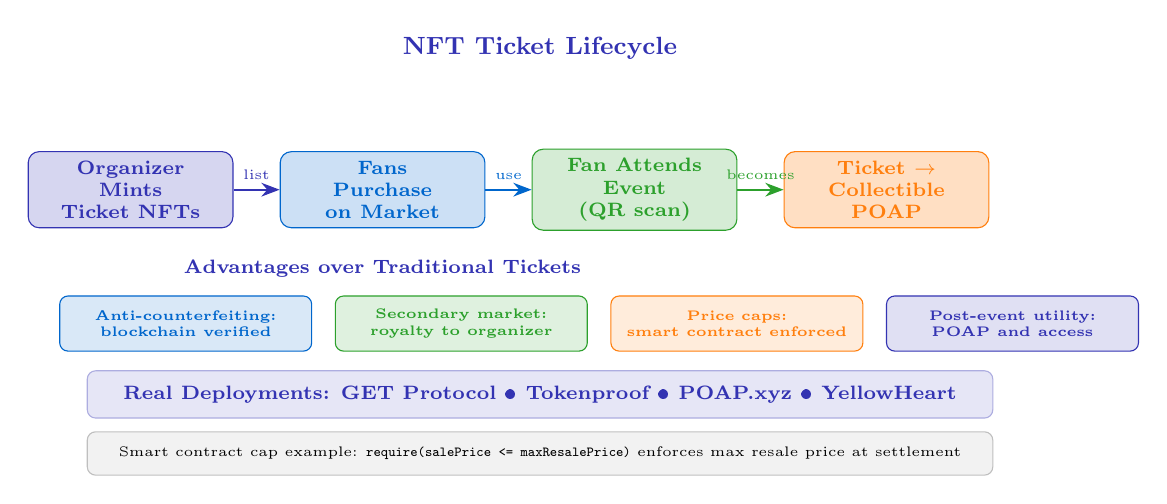
\begin{tikzpicture}[remember picture]
  \node[font=\small\bfseries, text=mlpurple] at (6.0,5.6) {NFT Ticket Lifecycle};

  %--- Event flow ---
  % Organizer mints
  \node[draw=mlpurple, fill=mlpurple!20, rounded corners=4pt, minimum width=2.6cm, minimum height=0.9cm, font=\scriptsize\bfseries, align=center, text=mlpurple] (org) at (0.8,3.8) {Organizer\\Mints\\Ticket NFTs};

  % Fans purchase
  \node[draw=mlblue, fill=mlblue!20, rounded corners=4pt, minimum width=2.6cm, minimum height=0.9cm, font=\scriptsize\bfseries, align=center, text=mlblue] (fans) at (4.0,3.8) {Fans\\Purchase\\on Market};

  % Attend event
  \node[draw=mlgreen, fill=mlgreen!20, rounded corners=4pt, minimum width=2.6cm, minimum height=0.9cm, font=\scriptsize\bfseries, align=center, text=mlgreen] (attend) at (7.2,3.8) {Fan Attends\\Event\\(QR scan)};

  % Ticket becomes POAP
  \node[draw=mlorange, fill=mlorange!25, rounded corners=4pt, minimum width=2.6cm, minimum height=0.9cm, font=\scriptsize\bfseries, align=center, text=mlorange] (poap) at (10.4,3.8) {Ticket $\to$\\Collectible\\POAP};

  \draw[-{Stealth}, thick, mlpurple] (org.east) -- node[above, font=\tiny] {list} (fans.west);
  \draw[-{Stealth}, thick, mlblue] (fans.east) -- node[above, font=\tiny] {use} (attend.west);
  \draw[-{Stealth}, thick, mlgreen] (attend.east) -- node[above, font=\tiny] {becomes} (poap.west);

  %--- Advantages ---
  \node[font=\scriptsize\bfseries, text=mlpurple] at (4.0,2.8) {Advantages over Traditional Tickets};

  \node[draw=mlblue, fill=mlblue!15, rounded corners=3pt, minimum width=3.2cm, minimum height=0.7cm, font=\tiny\bfseries, align=center, text=mlblue] at (1.5,2.1) {Anti-counterfeiting:\\blockchain verified};
  \node[draw=mlgreen, fill=mlgreen!15, rounded corners=3pt, minimum width=3.2cm, minimum height=0.7cm, font=\tiny\bfseries, align=center, text=mlgreen] at (5.0,2.1) {Secondary market:\\royalty to organizer};
  \node[draw=mlorange, fill=mlorange!15, rounded corners=3pt, minimum width=3.2cm, minimum height=0.7cm, font=\tiny\bfseries, align=center, text=mlorange] at (8.5,2.1) {Price caps:\\smart contract enforced};
  \node[draw=mlpurple, fill=mlpurple!15, rounded corners=3pt, minimum width=3.2cm, minimum height=0.7cm, font=\tiny\bfseries, align=center, text=mlpurple] at (12.0,2.1) {Post-event utility:\\POAP and access};

  %--- Real examples ---
  \node[draw=mllavender, fill=mllavender!30, rounded corners=3pt, minimum width=11.5cm, minimum height=0.6cm, font=\scriptsize\bfseries, align=center, text=mlpurple] at (6.0,1.2) {Real Deployments: GET Protocol \textbullet{} Tokenproof \textbullet{} POAP.xyz \textbullet{} YellowHeart};

  \node[draw=mlgray!50, fill=mlgray!10, rounded corners=3pt, minimum width=11.5cm, minimum height=0.55cm, font=\tiny, align=center] at (6.0,0.45) {Smart contract cap example: \texttt{require(salePrice <= maxResalePrice)} enforces max resale price at settlement};
\end{tikzpicture}
\bottomnote{NFT tickets solve counterfeiting while giving organizers control over secondary market pricing}
\end{frame}

% Frame 37: Intellectual Property and Licensing
\begin{frame}{Intellectual Property and Licensing}
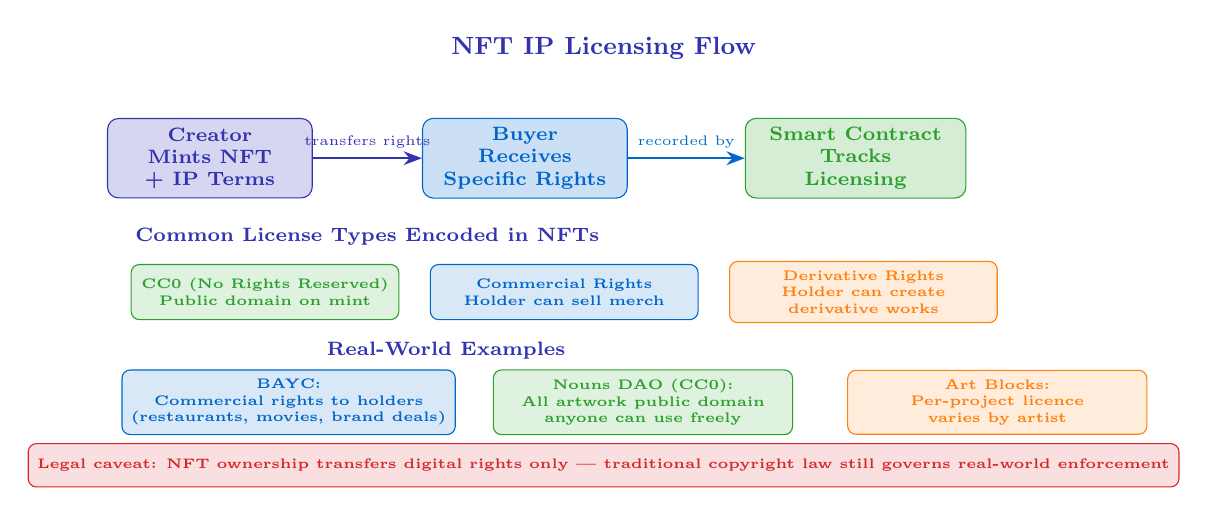
\begin{tikzpicture}[remember picture]
  \node[font=\small\bfseries, text=mlpurple] at (6.0,5.6) {NFT IP Licensing Flow};

  %--- IP flow ---
  % Creator
  \node[draw=mlpurple, fill=mlpurple!20, rounded corners=4pt, minimum width=2.6cm, minimum height=0.9cm, font=\scriptsize\bfseries, align=center, text=mlpurple] (creator) at (1.0,4.2) {Creator\\Mints NFT\\+ IP Terms};

  % Buyer
  \node[draw=mlblue, fill=mlblue!20, rounded corners=4pt, minimum width=2.6cm, minimum height=0.9cm, font=\scriptsize\bfseries, align=center, text=mlblue] (buyer) at (5.0,4.2) {Buyer\\Receives\\Specific Rights};

  % Smart contract
  \node[draw=mlgreen, fill=mlgreen!20, rounded corners=4pt, minimum width=2.8cm, minimum height=0.9cm, font=\scriptsize\bfseries, align=center, text=mlgreen] (sc) at (9.2,4.2) {Smart Contract\\Tracks\\Licensing};

  \draw[-{Stealth}, thick, mlpurple] (creator.east) -- node[above, font=\tiny] {transfers rights} (buyer.west);
  \draw[-{Stealth}, thick, mlblue] (buyer.east) -- node[above, font=\tiny] {recorded by} (sc.west);

  %--- License types ---
  \node[font=\scriptsize\bfseries, text=mlpurple] at (3.0,3.2) {Common License Types Encoded in NFTs};

  \node[draw=mlgreen, fill=mlgreen!15, rounded corners=3pt, minimum width=3.4cm, minimum height=0.7cm, font=\tiny\bfseries, align=center, text=mlgreen] at (1.7,2.5) {CC0 (No Rights Reserved)\\Public domain on mint};
  \node[draw=mlblue, fill=mlblue!15, rounded corners=3pt, minimum width=3.4cm, minimum height=0.7cm, font=\tiny\bfseries, align=center, text=mlblue] at (5.5,2.5) {Commercial Rights\\Holder can sell merch};
  \node[draw=mlorange, fill=mlorange!15, rounded corners=3pt, minimum width=3.4cm, minimum height=0.7cm, font=\tiny\bfseries, align=center, text=mlorange] at (9.3,2.5) {Derivative Rights\\Holder can create\\derivative works};

  %--- Examples ---
  \node[font=\scriptsize\bfseries, text=mlpurple] at (4.0,1.75) {Real-World Examples};

  \node[draw=mlblue, fill=mlblue!15, rounded corners=3pt, minimum width=3.8cm, minimum height=0.65cm, font=\tiny\bfseries, align=center, text=mlblue] at (2.0,1.1) {BAYC:\\Commercial rights to holders\\(restaurants, movies, brand deals)};
  \node[draw=mlgreen, fill=mlgreen!15, rounded corners=3pt, minimum width=3.8cm, minimum height=0.65cm, font=\tiny\bfseries, align=center, text=mlgreen] at (6.5,1.1) {Nouns DAO (CC0):\\All artwork public domain\\anyone can use freely};
  \node[draw=mlorange, fill=mlorange!15, rounded corners=3pt, minimum width=3.8cm, minimum height=0.65cm, font=\tiny\bfseries, align=center, text=mlorange] at (11.0,1.1) {Art Blocks:\\Per-project licence\\varies by artist};

  \node[draw=mlred, fill=mlred!15, rounded corners=3pt, minimum width=11.5cm, minimum height=0.55cm, font=\tiny\bfseries, align=center, text=mlred] at (6.0,0.3) {Legal caveat: NFT ownership transfers digital rights only --- traditional copyright law still governs real-world enforcement};
\end{tikzpicture}
\bottomnote{NFTs can encode intellectual property rights -- but legal enforcement is still evolving}
\end{frame}

% Frame 38: Section 3 Summary
\begin{frame}{Section 3 Summary}
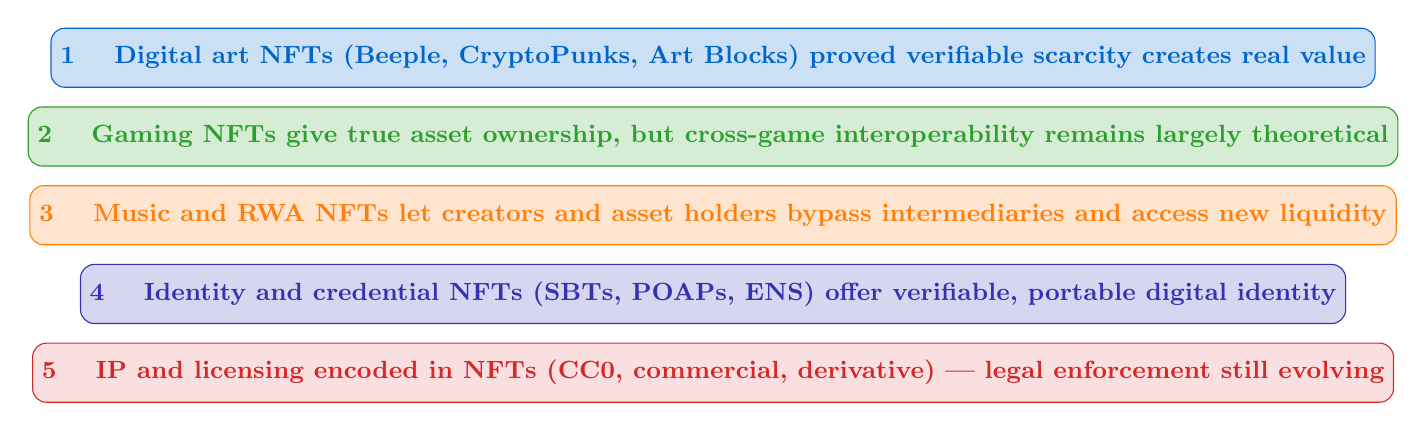
\begin{tikzpicture}[remember picture]
  \node[draw=mlblue, fill=mlblue!20, rounded corners=5pt, minimum width=11.6cm, minimum height=0.75cm, font=\small\bfseries, align=center, text=mlblue] at (6.0,5.2) {1 \quad Digital art NFTs (Beeple, CryptoPunks, Art Blocks) proved verifiable scarcity creates real value};
  \node[draw=mlgreen, fill=mlgreen!20, rounded corners=5pt, minimum width=11.6cm, minimum height=0.75cm, font=\small\bfseries, align=center, text=mlgreen] at (6.0,4.2) {2 \quad Gaming NFTs give true asset ownership, but cross-game interoperability remains largely theoretical};
  \node[draw=mlorange, fill=mlorange!20, rounded corners=5pt, minimum width=11.6cm, minimum height=0.75cm, font=\small\bfseries, align=center, text=mlorange] at (6.0,3.2) {3 \quad Music and RWA NFTs let creators and asset holders bypass intermediaries and access new liquidity};
  \node[draw=mlpurple, fill=mlpurple!20, rounded corners=5pt, minimum width=11.6cm, minimum height=0.75cm, font=\small\bfseries, align=center, text=mlpurple] at (6.0,2.2) {4 \quad Identity and credential NFTs (SBTs, POAPs, ENS) offer verifiable, portable digital identity};
  \node[draw=mlred, fill=mlred!15, rounded corners=5pt, minimum width=11.6cm, minimum height=0.75cm, font=\small\bfseries, align=center, text=mlred] at (6.0,1.2) {5 \quad IP and licensing encoded in NFTs (CC0, commercial, derivative) --- legal enforcement still evolving};
\end{tikzpicture}
\bottomnote{Section 3 complete -- next: NFT Valuation \& Analytics}
\end{frame}

%% ============================================================
%% SECTION 4: NFT VALUATION & ANALYTICS
%% ============================================================
\section{NFT Valuation \& Analytics}

% Frame 39: Section 4 Divider
\begin{frame}{Section 4: NFT Valuation \& Analytics}
\begin{beamercolorbox}[sep=12pt,center,rounded=true,shadow=true]{palette quaternary}
  {\Large\bfseries Section 4: NFT Valuation \& Analytics}\\[4pt]
  {\normalsize Rarity scoring, floor price analysis, wash trading detection, and market metrics}
\end{beamercolorbox}

\vspace{4mm}
\begin{columns}[T]
\column{0.55\textwidth}
\begin{block}{What You Will Learn}
\begin{itemize}\setlength{\itemsep}{2pt}
  \item Why NFT valuation differs fundamentally from traditional finance
  \item Rarity scoring methods and how to calculate rarity scores
  \item Floor price trends and support/resistance analysis
  \item Core market metrics: holders, listings, volume, royalties
  \item Wash trading detection and index construction
\end{itemize}
\end{block}
\column{0.42\textwidth}
\begin{block}{Frames in This Section}
\begin{itemize}\setlength{\itemsep}{1pt}
  \item Frame 39 --- Section overview
  \item Frame 40 --- Valuation challenges
  \item Frame 41 --- Rarity scoring methods
  \item Frame 42 --- Rarity worked example
  \item Frame 43 --- Floor price analysis
  \item Frame 44 --- Market metrics table
  \item Frame 45 --- Wash trading analytics
  \item Frame 46 --- NFT index construction
  \item Frame 47 --- Portfolio analysis
  \item Frame 48 --- Section 4 summary
\end{itemize}
\end{block}
\end{columns}
\bottomnote{Section 4 | Frames 39--48 | NFT Valuation \& Analytics}
\end{frame}

% Frame 40: NFT Valuation Challenges
\begin{frame}{NFT Valuation Challenges}
\begin{columns}[T]
\column{0.47\textwidth}
\begin{block}{Why NFTs Are Hard to Value}
\begin{itemize}\setlength{\itemsep}{3pt}
  \item \textbf{Illiquidity} --- few comparable sales; thin markets
  \item \textbf{Subjectivity} --- aesthetic and cultural value is unquantifiable
  \item \textbf{Wash trading distortion} --- artificial volume inflates perceived demand
  \item \textbf{No cash flows} --- no dividends, no earnings, no DCF anchor
  \item \textbf{Thin markets} --- one-sided order books, wide bid-ask spreads
\end{itemize}
\end{block}

\column{0.50\textwidth}
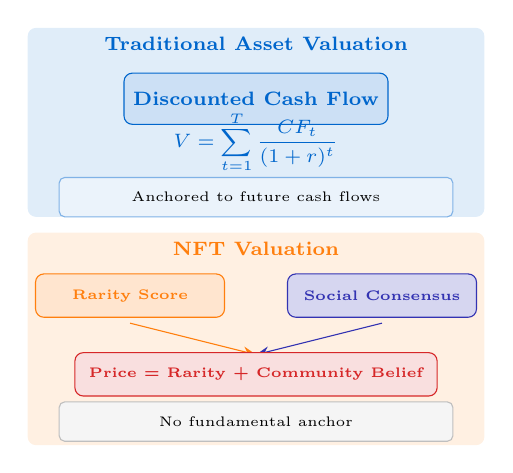
\begin{tikzpicture}[remember picture]
  % Traditional asset panel
  \fill[mlblue!12, rounded corners=3pt] (0,3.1) rectangle (5.8,5.5);
  \node[font=\scriptsize\bfseries, text=mlblue] at (2.9,5.3) {Traditional Asset Valuation};

  \node[draw=mlblue, fill=mlblue!20, rounded corners=3pt, minimum width=2.4cm, minimum height=0.65cm, font=\scriptsize\bfseries, align=center, text=mlblue] at (2.9,4.6) {Discounted Cash Flow};

  \node[font=\scriptsize, text=mlblue, align=center] at (2.9,4.05) {$V = \displaystyle\sum_{t=1}^{T} \frac{CF_t}{(1+r)^t}$};

  \node[draw=mlblue!50, fill=mlblue!8, rounded corners=2pt, minimum width=5.0cm, minimum height=0.5cm, font=\tiny, align=center] at (2.9,3.35) {Anchored to future cash flows};

  % NFT panel
  \fill[mlorange!12, rounded corners=3pt] (0,0.2) rectangle (5.8,2.9);
  \node[font=\scriptsize\bfseries, text=mlorange] at (2.9,2.7) {NFT Valuation};

  \node[draw=mlorange, fill=mlorange!20, rounded corners=3pt, minimum width=2.4cm, minimum height=0.55cm, font=\tiny\bfseries, align=center, text=mlorange] at (1.3,2.1) {Rarity Score};
  \node[draw=mlpurple, fill=mlpurple!20, rounded corners=3pt, minimum width=2.4cm, minimum height=0.55cm, font=\tiny\bfseries, align=center, text=mlpurple] at (4.5,2.1) {Social Consensus};

  \draw[-{Stealth}, thin, mlorange] (1.3,1.75) -- (2.9,1.35);
  \draw[-{Stealth}, thin, mlpurple] (4.5,1.75) -- (2.9,1.35);

  \node[draw=mlred, fill=mlred!15, rounded corners=3pt, minimum width=4.6cm, minimum height=0.55cm, font=\tiny\bfseries, align=center, text=mlred] at (2.9,1.1) {Price = Rarity + Community Belief};

  \node[draw=mlgray!50, fill=mlgray!8, rounded corners=2pt, minimum width=5.0cm, minimum height=0.5cm, font=\tiny, align=center] at (2.9,0.5) {No fundamental anchor};
\end{tikzpicture}
\end{columns}
\bottomnote{NFT valuation is fundamentally different from traditional finance -- there are no discounted cash flow models}
\end{frame}

% Frame 41: Rarity Scoring Methods
\begin{frame}{Rarity Scoring Methods}
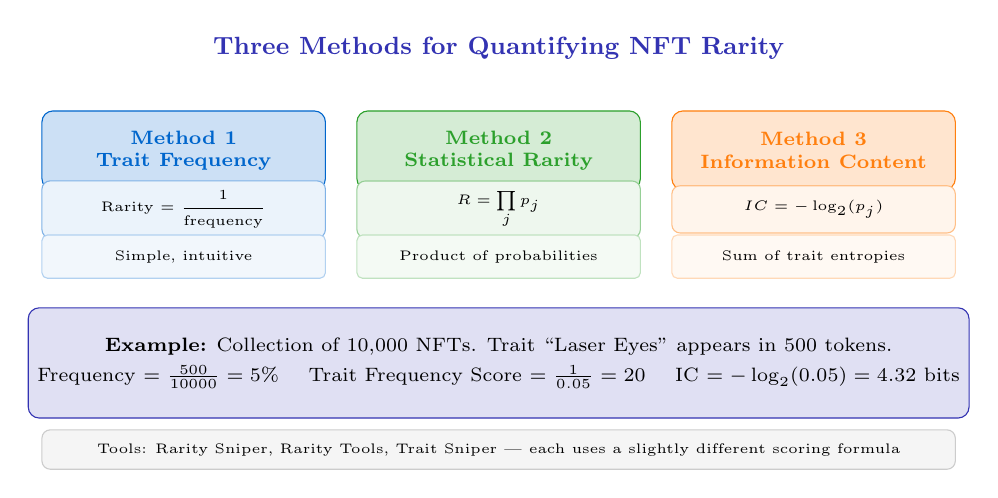
\begin{tikzpicture}[remember picture]
  \node[font=\small\bfseries, text=mlpurple] at (6.0,5.6) {Three Methods for Quantifying NFT Rarity};

  % Method 1: Trait Frequency
  \node[draw=mlblue, fill=mlblue!20, rounded corners=4pt, minimum width=3.6cm, minimum height=1.0cm, font=\scriptsize\bfseries, align=center, text=mlblue] (m1) at (2.0,4.3) {Method 1\\Trait Frequency};
  \node[draw=mlblue!50, fill=mlblue!8, rounded corners=3pt, minimum width=3.6cm, minimum height=0.6cm, font=\tiny, align=center] (m1d) at (2.0,3.55) {Rarity $=\dfrac{1}{\text{frequency}}$};
  \node[draw=mlblue!30, fill=mlblue!5, rounded corners=2pt, minimum width=3.6cm, minimum height=0.55cm, font=\tiny, align=center] at (2.0,2.95) {Simple, intuitive};

  % Method 2: Statistical Rarity
  \node[draw=mlgreen, fill=mlgreen!20, rounded corners=4pt, minimum width=3.6cm, minimum height=1.0cm, font=\scriptsize\bfseries, align=center, text=mlgreen] (m2) at (6.0,4.3) {Method 2\\Statistical Rarity};
  \node[draw=mlgreen!50, fill=mlgreen!8, rounded corners=3pt, minimum width=3.6cm, minimum height=0.6cm, font=\tiny, align=center] (m2d) at (6.0,3.55) {$R = \displaystyle\prod_{j} p_j$};
  \node[draw=mlgreen!30, fill=mlgreen!5, rounded corners=2pt, minimum width=3.6cm, minimum height=0.55cm, font=\tiny, align=center] at (6.0,2.95) {Product of probabilities};

  % Method 3: Information Content
  \node[draw=mlorange, fill=mlorange!20, rounded corners=4pt, minimum width=3.6cm, minimum height=1.0cm, font=\scriptsize\bfseries, align=center, text=mlorange] (m3) at (10.0,4.3) {Method 3\\Information Content};
  \node[draw=mlorange!50, fill=mlorange!8, rounded corners=3pt, minimum width=3.6cm, minimum height=0.6cm, font=\tiny, align=center] (m3d) at (10.0,3.55) {$IC = -\log_2(p_j)$};
  \node[draw=mlorange!30, fill=mlorange!5, rounded corners=2pt, minimum width=3.6cm, minimum height=0.55cm, font=\tiny, align=center] at (10.0,2.95) {Sum of trait entropies};

  % Worked example box
  \node[draw=mlpurple, fill=mlpurple!15, rounded corners=4pt, minimum width=11.6cm, minimum height=1.4cm, font=\scriptsize, align=center] at (6.0,1.6) {%
    \textbf{Example:} Collection of 10{,}000 NFTs. Trait ``Laser Eyes'' appears in 500 tokens.\\[3pt]
    Frequency $= \frac{500}{10000} = 5\%$ \quad
    Trait Frequency Score $= \frac{1}{0.05} = 20$ \quad
    IC $= -\log_2(0.05) = 4.32$ bits
  };

  \node[draw=mlgray!40, fill=mlgray!8, rounded corners=3pt, minimum width=11.6cm, minimum height=0.5cm, font=\tiny, align=center] at (6.0,0.5) {Tools: Rarity Sniper, Rarity Tools, Trait Sniper --- each uses a slightly different scoring formula};
\end{tikzpicture}
\bottomnote{Rarity scores quantify how uncommon an NFT's trait combination is within its collection}
\end{frame}

% Frame 42: Rarity Score Worked Example
\begin{frame}{Rarity Score: Worked Example}
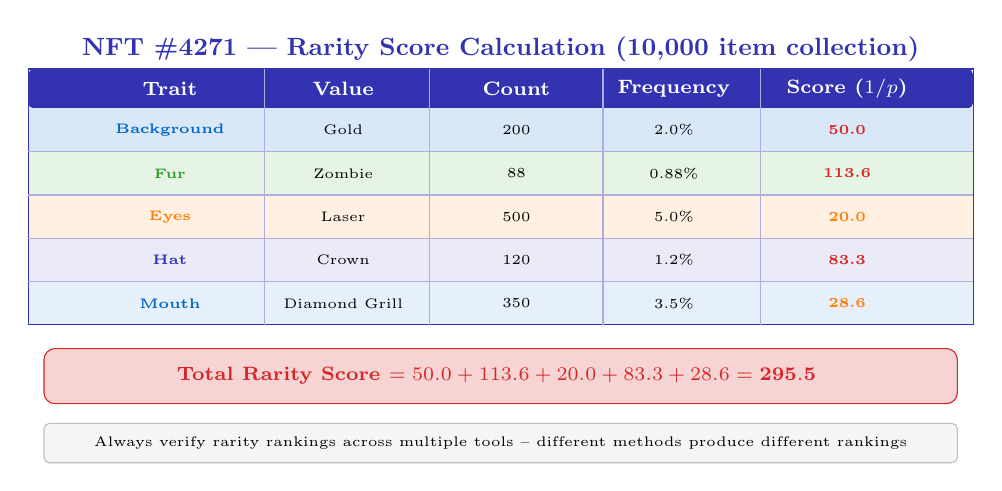
\begin{tikzpicture}[remember picture]
  \node[font=\small\bfseries, text=mlpurple] at (6.0,5.6) {NFT \#4271 --- Rarity Score Calculation (10{,}000 item collection)};

  % Header row
  \fill[mlpurple, rounded corners=2pt] (0,4.85) rectangle (12.0,5.35);
  \node[font=\scriptsize\bfseries, text=white, align=center] at (1.8,5.1) {Trait};
  \node[font=\scriptsize\bfseries, text=white, align=center] at (4.0,5.1) {Value};
  \node[font=\scriptsize\bfseries, text=white, align=center] at (6.2,5.1) {Count};
  \node[font=\scriptsize\bfseries, text=white, align=center] at (8.2,5.1) {Frequency};
  \node[font=\scriptsize\bfseries, text=white, align=center] at (10.4,5.1) {Score ($1/p$)};

  % Row 1
  \fill[mlblue!15] (0,4.3) rectangle (12.0,4.85);
  \node[font=\tiny\bfseries, text=mlblue, align=center] at (1.8,4.575) {Background};
  \node[font=\tiny, align=center] at (4.0,4.575) {Gold};
  \node[font=\tiny, align=center] at (6.2,4.575) {200};
  \node[font=\tiny, align=center] at (8.2,4.575) {2.0\%};
  \node[font=\tiny\bfseries, text=mlred, align=center] at (10.4,4.575) {50.0};

  % Row 2
  \fill[mlgreen!12] (0,3.75) rectangle (12.0,4.3);
  \node[font=\tiny\bfseries, text=mlgreen, align=center] at (1.8,4.025) {Fur};
  \node[font=\tiny, align=center] at (4.0,4.025) {Zombie};
  \node[font=\tiny, align=center] at (6.2,4.025) {88};
  \node[font=\tiny, align=center] at (8.2,4.025) {0.88\%};
  \node[font=\tiny\bfseries, text=mlred, align=center] at (10.4,4.025) {113.6};

  % Row 3
  \fill[mlorange!12] (0,3.2) rectangle (12.0,3.75);
  \node[font=\tiny\bfseries, text=mlorange, align=center] at (1.8,3.475) {Eyes};
  \node[font=\tiny, align=center] at (4.0,3.475) {Laser};
  \node[font=\tiny, align=center] at (6.2,3.475) {500};
  \node[font=\tiny, align=center] at (8.2,3.475) {5.0\%};
  \node[font=\tiny\bfseries, text=mlorange, align=center] at (10.4,3.475) {20.0};

  % Row 4
  \fill[mlpurple!10] (0,2.65) rectangle (12.0,3.2);
  \node[font=\tiny\bfseries, text=mlpurple, align=center] at (1.8,2.925) {Hat};
  \node[font=\tiny, align=center] at (4.0,2.925) {Crown};
  \node[font=\tiny, align=center] at (6.2,2.925) {120};
  \node[font=\tiny, align=center] at (8.2,2.925) {1.2\%};
  \node[font=\tiny\bfseries, text=mlred, align=center] at (10.4,2.925) {83.3};

  % Row 5
  \fill[mlblue!10] (0,2.1) rectangle (12.0,2.65);
  \node[font=\tiny\bfseries, text=mlblue, align=center] at (1.8,2.375) {Mouth};
  \node[font=\tiny, align=center] at (4.0,2.375) {Diamond Grill};
  \node[font=\tiny, align=center] at (6.2,2.375) {350};
  \node[font=\tiny, align=center] at (8.2,2.375) {3.5\%};
  \node[font=\tiny\bfseries, text=mlorange, align=center] at (10.4,2.375) {28.6};

  % Border and column lines
  \draw[mlpurple, thin] (0,2.1) rectangle (12.0,5.35);
  \draw[mlpurple!40, thin] (3.0,2.1) -- (3.0,5.35);
  \draw[mlpurple!40, thin] (5.1,2.1) -- (5.1,5.35);
  \draw[mlpurple!40, thin] (7.3,2.1) -- (7.3,5.35);
  \draw[mlpurple!40, thin] (9.3,2.1) -- (9.3,5.35);
  \draw[mlpurple!40, thin] (0,2.65) -- (12.0,2.65);
  \draw[mlpurple!40, thin] (0,3.2) -- (12.0,3.2);
  \draw[mlpurple!40, thin] (0,3.75) -- (12.0,3.75);
  \draw[mlpurple!40, thin] (0,4.3) -- (12.0,4.3);

  % Total score box
  \node[draw=mlred, fill=mlred!20, rounded corners=4pt, minimum width=11.6cm, minimum height=0.7cm, font=\scriptsize\bfseries, align=center, text=mlred] at (6.0,1.45) {%
    Total Rarity Score $= 50.0 + 113.6 + 20.0 + 83.3 + 28.6 = \mathbf{295.5}$
  };

  \node[draw=mlgray!50, fill=mlgray!8, rounded corners=2pt, minimum width=11.6cm, minimum height=0.5cm, font=\tiny, align=center] at (6.0,0.6) {Always verify rarity rankings across multiple tools -- different methods produce different rankings};
\end{tikzpicture}
\bottomnote{Always verify rarity rankings across multiple tools -- different methods produce different rankings}
\end{frame}

% Frame 43: Floor Price Analysis
\begin{frame}{Floor Price Analysis}
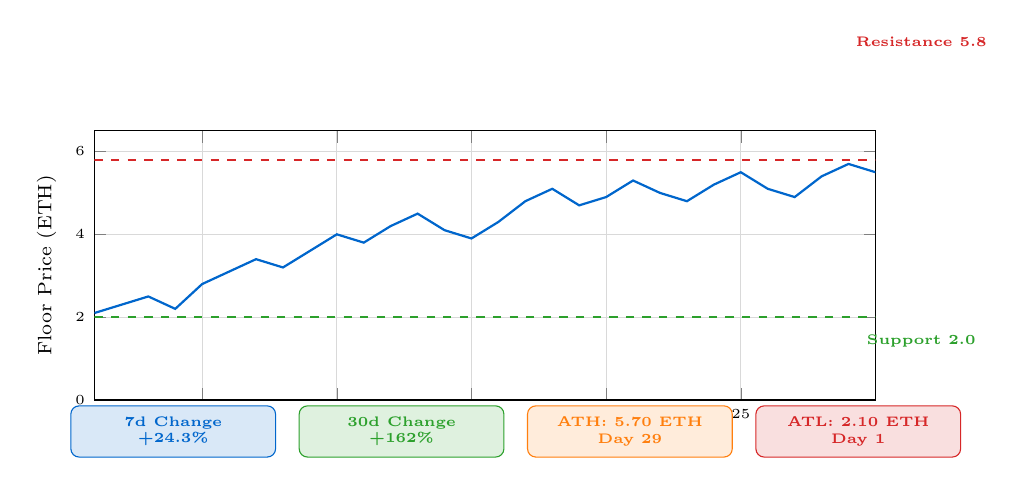
\begin{tikzpicture}[remember picture]
  \begin{axis}[
    at={(0.3cm,0.8cm)},
    width=11.5cm,
    height=5.0cm,
    xlabel={Day},
    ylabel={Floor Price (ETH)},
    xlabel style={font=\scriptsize},
    ylabel style={font=\scriptsize},
    xtick={1,5,10,15,20,25,30},
    xticklabels={1,5,10,15,20,25,30},
    tick label style={font=\tiny},
    ymin=0, ymax=6.5,
    xmin=1, xmax=30,
    grid=major,
    grid style={mlgray!30},
  ]
    \addplot[thick, mlblue, mark=none] coordinates {
      (1,2.1)(2,2.3)(3,2.5)(4,2.2)(5,2.8)(6,3.1)(7,3.4)(8,3.2)(9,3.6)(10,4.0)
      (11,3.8)(12,4.2)(13,4.5)(14,4.1)(15,3.9)(16,4.3)(17,4.8)(18,5.1)(19,4.7)(20,4.9)
      (21,5.3)(22,5.0)(23,4.8)(24,5.2)(25,5.5)(26,5.1)(27,4.9)(28,5.4)(29,5.7)(30,5.5)
    };
    \addplot[dashed, mlgreen, thick, mark=none] coordinates {(1,2.0)(30,2.0)};
    \addplot[dashed, mlred, thick, mark=none] coordinates {(1,5.8)(30,5.8)};
  \end{axis}
  % Labels
  \node[font=\tiny\bfseries, text=mlgreen] at (10.8,1.55) {Support 2.0};
  \node[font=\tiny\bfseries, text=mlred] at (10.8,5.35) {Resistance 5.8};

  % Metric boxes
  \node[draw=mlblue, fill=mlblue!15, rounded corners=3pt, minimum width=2.6cm, minimum height=0.65cm, font=\tiny\bfseries, align=center, text=mlblue] at (1.3,0.4) {7d Change\\+24.3\%};
  \node[draw=mlgreen, fill=mlgreen!15, rounded corners=3pt, minimum width=2.6cm, minimum height=0.65cm, font=\tiny\bfseries, align=center, text=mlgreen] at (4.2,0.4) {30d Change\\+162\%};
  \node[draw=mlorange, fill=mlorange!15, rounded corners=3pt, minimum width=2.6cm, minimum height=0.65cm, font=\tiny\bfseries, align=center, text=mlorange] at (7.1,0.4) {ATH: 5.70 ETH\\Day 29};
  \node[draw=mlred, fill=mlred!15, rounded corners=3pt, minimum width=2.6cm, minimum height=0.65cm, font=\tiny\bfseries, align=center, text=mlred] at (10.0,0.4) {ATL: 2.10 ETH\\Day 1};
\end{tikzpicture}
\bottomnote{Floor price trends reveal market sentiment -- sustained floor above previous lows signals strength}
\end{frame}

% Frame 44: NFT Market Metrics Table
\begin{frame}{NFT Market Metrics}
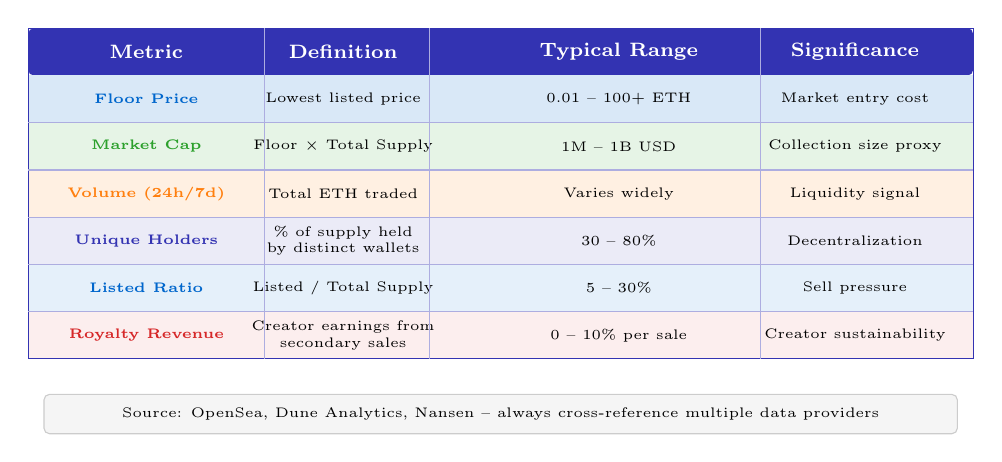
\begin{tikzpicture}[remember picture]
  % Header
  \fill[mlpurple, rounded corners=2pt] (0,5.1) rectangle (12.0,5.7);
  \node[font=\scriptsize\bfseries, text=white, align=center] at (1.5,5.4) {Metric};
  \node[font=\scriptsize\bfseries, text=white, align=center] at (4.0,5.4) {Definition};
  \node[font=\scriptsize\bfseries, text=white, align=center] at (7.5,5.4) {Typical Range};
  \node[font=\scriptsize\bfseries, text=white, align=center] at (10.5,5.4) {Significance};

  % Row 1: Floor Price
  \fill[mlblue!15] (0,4.5) rectangle (12.0,5.1);
  \node[font=\tiny\bfseries, text=mlblue, align=center] at (1.5,4.8) {Floor Price};
  \node[font=\tiny, align=center] at (4.0,4.8) {Lowest listed price};
  \node[font=\tiny, align=center] at (7.5,4.8) {0.01 -- 100+ ETH};
  \node[font=\tiny, align=center] at (10.5,4.8) {Market entry cost};

  % Row 2: Market Cap
  \fill[mlgreen!12] (0,3.9) rectangle (12.0,4.5);
  \node[font=\tiny\bfseries, text=mlgreen, align=center] at (1.5,4.2) {Market Cap};
  \node[font=\tiny, align=center] at (4.0,4.2) {Floor $\times$ Total Supply};
  \node[font=\tiny, align=center] at (7.5,4.2) {1M -- 1B USD};
  \node[font=\tiny, align=center] at (10.5,4.2) {Collection size proxy};

  % Row 3: Volume
  \fill[mlorange!12] (0,3.3) rectangle (12.0,3.9);
  \node[font=\tiny\bfseries, text=mlorange, align=center] at (1.5,3.6) {Volume (24h/7d)};
  \node[font=\tiny, align=center] at (4.0,3.6) {Total ETH traded};
  \node[font=\tiny, align=center] at (7.5,3.6) {Varies widely};
  \node[font=\tiny, align=center] at (10.5,3.6) {Liquidity signal};

  % Row 4: Unique Holders
  \fill[mlpurple!10] (0,2.7) rectangle (12.0,3.3);
  \node[font=\tiny\bfseries, text=mlpurple, align=center] at (1.5,3.0) {Unique Holders};
  \node[font=\tiny, align=center] at (4.0,3.0) {\% of supply held\\by distinct wallets};
  \node[font=\tiny, align=center] at (7.5,3.0) {30 -- 80\%};
  \node[font=\tiny, align=center] at (10.5,3.0) {Decentralization};

  % Row 5: Listed Ratio
  \fill[mlblue!10] (0,2.1) rectangle (12.0,2.7);
  \node[font=\tiny\bfseries, text=mlblue, align=center] at (1.5,2.4) {Listed Ratio};
  \node[font=\tiny, align=center] at (4.0,2.4) {Listed / Total Supply};
  \node[font=\tiny, align=center] at (7.5,2.4) {5 -- 30\%};
  \node[font=\tiny, align=center] at (10.5,2.4) {Sell pressure};

  % Row 6: Royalty Revenue
  \fill[mlred!8] (0,1.5) rectangle (12.0,2.1);
  \node[font=\tiny\bfseries, text=mlred, align=center] at (1.5,1.8) {Royalty Revenue};
  \node[font=\tiny, align=center] at (4.0,1.8) {Creator earnings from\\secondary sales};
  \node[font=\tiny, align=center] at (7.5,1.8) {0 -- 10\% per sale};
  \node[font=\tiny, align=center] at (10.5,1.8) {Creator sustainability};

  % Border and lines
  \draw[mlpurple, thin] (0,1.5) rectangle (12.0,5.7);
  \draw[mlpurple!40, thin] (3.0,1.5) -- (3.0,5.7);
  \draw[mlpurple!40, thin] (5.1,1.5) -- (5.1,5.7);
  \draw[mlpurple!40, thin] (9.3,1.5) -- (9.3,5.7);
  \draw[mlpurple!40, thin] (0,2.1) -- (12.0,2.1);
  \draw[mlpurple!40, thin] (0,2.7) -- (12.0,2.7);
  \draw[mlpurple!40, thin] (0,3.3) -- (12.0,3.3);
  \draw[mlpurple!40, thin] (0,3.9) -- (12.0,3.9);
  \draw[mlpurple!40, thin] (0,4.5) -- (12.0,4.5);

  \node[draw=mlgray!40, fill=mlgray!8, rounded corners=2pt, minimum width=11.6cm, minimum height=0.5cm, font=\tiny, align=center] at (6.0,0.8) {Source: OpenSea, Dune Analytics, Nansen -- always cross-reference multiple data providers};
\end{tikzpicture}
\bottomnote{These six metrics provide a quantitative framework for evaluating any NFT collection}
\end{frame}

% Frame 45: Wash Trading Analytics
\begin{frame}{Wash Trading Analytics}
\begin{columns}[T]
\column{0.52\textwidth}
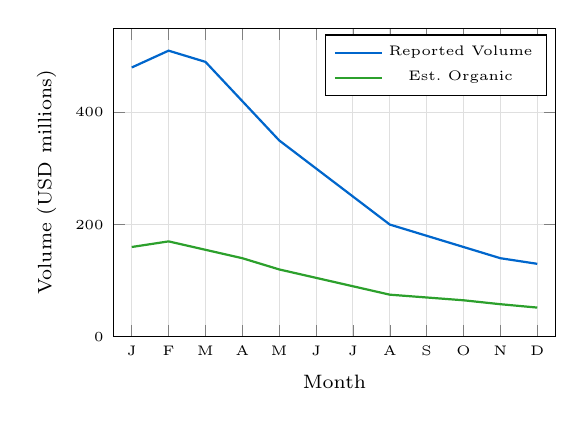
\begin{tikzpicture}[remember picture]
  \begin{axis}[
    at={(0cm,0cm)},
    width=7.2cm,
    height=5.5cm,
    xlabel={Month},
    ylabel={Volume (USD millions)},
    xlabel style={font=\scriptsize},
    ylabel style={font=\scriptsize},
    xtick={1,2,3,4,5,6,7,8,9,10,11,12},
    xticklabels={J,F,M,A,M,J,J,A,S,O,N,D},
    tick label style={font=\tiny},
    ymin=0, ymax=550,
    xmin=0.5, xmax=12.5,
    grid=major,
    grid style={mlgray!25},
    legend style={font=\tiny, at={(0.98,0.98)}, anchor=north east},
  ]
    \addplot[thick, mlblue, mark=none] coordinates {
      (1,480)(2,510)(3,490)(4,420)(5,350)(6,300)(7,250)(8,200)(9,180)(10,160)(11,140)(12,130)
    };
    \addlegendentry{Reported Volume};
    \addplot[thick, mlgreen, mark=none] coordinates {
      (1,160)(2,170)(3,155)(4,140)(5,120)(6,105)(7,90)(8,75)(9,70)(10,65)(11,58)(12,52)
    };
    \addlegendentry{Est.\ Organic};
  \end{axis}
\end{tikzpicture}

\column{0.45\textwidth}
\begin{block}{Detection Heuristics}
\begin{itemize}\setlength{\itemsep}{3pt}
  \item \textbf{Self-trading} --- same wallet buys back its own NFT
  \item \textbf{Circular patterns} --- A sells to B, B sells to C, C sells to A
  \item \textbf{Unprofitable trades} --- buyer pays more than seller received (after gas)
  \item \textbf{Funding source analysis} --- wallets funded from same exchange withdraw
\end{itemize}
\end{block}
\vspace{3mm}
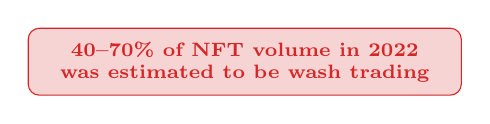
\begin{tikzpicture}[remember picture]
  \node[draw=mlred, fill=mlred!20, rounded corners=4pt, minimum width=5.5cm, minimum height=0.85cm, font=\scriptsize\bfseries, align=center, text=mlred] at (2.75,0.42) {40--70\% of NFT volume in 2022\\was estimated to be wash trading};
\end{tikzpicture}
\end{columns}
\bottomnote{Research estimates 40-70\% of NFT trading volume in 2022 was wash trading}
\end{frame}

% Frame 46: NFT Index Construction
\begin{frame}{NFT Index Construction}
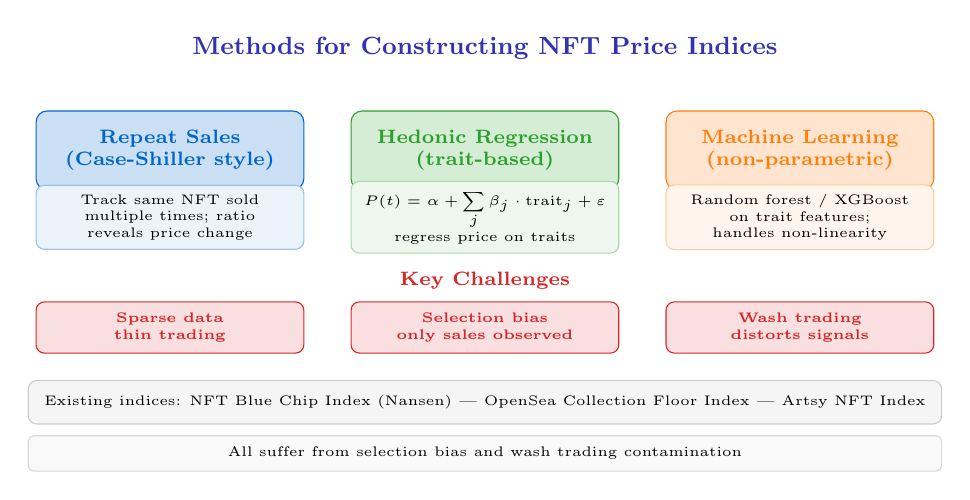
\begin{tikzpicture}[remember picture]
  \node[font=\small\bfseries, text=mlpurple] at (6.0,5.6) {Methods for Constructing NFT Price Indices};

  % Method 1: Repeat Sales
  \node[draw=mlblue, fill=mlblue!20, rounded corners=4pt, minimum width=3.4cm, minimum height=1.0cm, font=\scriptsize\bfseries, align=center, text=mlblue] (r1) at (2.0,4.3) {Repeat Sales\\(Case-Shiller style)};
  \node[draw=mlblue!40, fill=mlblue!8, rounded corners=3pt, minimum width=3.4cm, minimum height=0.7cm, font=\tiny, align=center] at (2.0,3.45) {Track same NFT sold\\multiple times; ratio\\reveals price change};

  % Method 2: Hedonic Regression
  \node[draw=mlgreen, fill=mlgreen!20, rounded corners=4pt, minimum width=3.4cm, minimum height=1.0cm, font=\scriptsize\bfseries, align=center, text=mlgreen] (r2) at (6.0,4.3) {Hedonic Regression\\(trait-based)};
  \node[draw=mlgreen!40, fill=mlgreen!8, rounded corners=3pt, minimum width=3.4cm, minimum height=0.7cm, font=\tiny, align=center] at (6.0,3.45) {$P(t) = \alpha + \displaystyle\sum_{j} \beta_j \cdot \text{trait}_j + \varepsilon$\\regress price on traits};

  % Method 3: Machine Learning
  \node[draw=mlorange, fill=mlorange!20, rounded corners=4pt, minimum width=3.4cm, minimum height=1.0cm, font=\scriptsize\bfseries, align=center, text=mlorange] (r3) at (10.0,4.3) {Machine Learning\\(non-parametric)};
  \node[draw=mlorange!40, fill=mlorange!8, rounded corners=3pt, minimum width=3.4cm, minimum height=0.7cm, font=\tiny, align=center] at (10.0,3.45) {Random forest / XGBoost\\on trait features;\\handles non-linearity};

  % Issues
  \node[font=\scriptsize\bfseries, text=mlred] at (6.0,2.65) {Key Challenges};

  \node[draw=mlred, fill=mlred!15, rounded corners=3pt, minimum width=3.4cm, minimum height=0.65cm, font=\tiny\bfseries, align=center, text=mlred] at (2.0,2.05) {Sparse data\\thin trading};
  \node[draw=mlred, fill=mlred!15, rounded corners=3pt, minimum width=3.4cm, minimum height=0.65cm, font=\tiny\bfseries, align=center, text=mlred] at (6.0,2.05) {Selection bias\\only sales observed};
  \node[draw=mlred, fill=mlred!15, rounded corners=3pt, minimum width=3.4cm, minimum height=0.65cm, font=\tiny\bfseries, align=center, text=mlred] at (10.0,2.05) {Wash trading\\distorts signals};

  \node[draw=mlgray!40, fill=mlgray!8, rounded corners=3pt, minimum width=11.6cm, minimum height=0.55cm, font=\tiny, align=center] at (6.0,1.1) {Existing indices: NFT Blue Chip Index (Nansen) | OpenSea Collection Floor Index | Artsy NFT Index};
  \node[draw=mlgray!30, fill=mlgray!5, rounded corners=2pt, minimum width=11.6cm, minimum height=0.45cm, font=\tiny, align=center] at (6.0,0.45) {All suffer from selection bias and wash trading contamination};
\end{tikzpicture}
\bottomnote{NFT indices are essential for portfolio analysis but face sparse data and selection bias}
\end{frame}

% Frame 47: Portfolio Analysis with NFTs
\begin{frame}{Portfolio Analysis with NFTs}
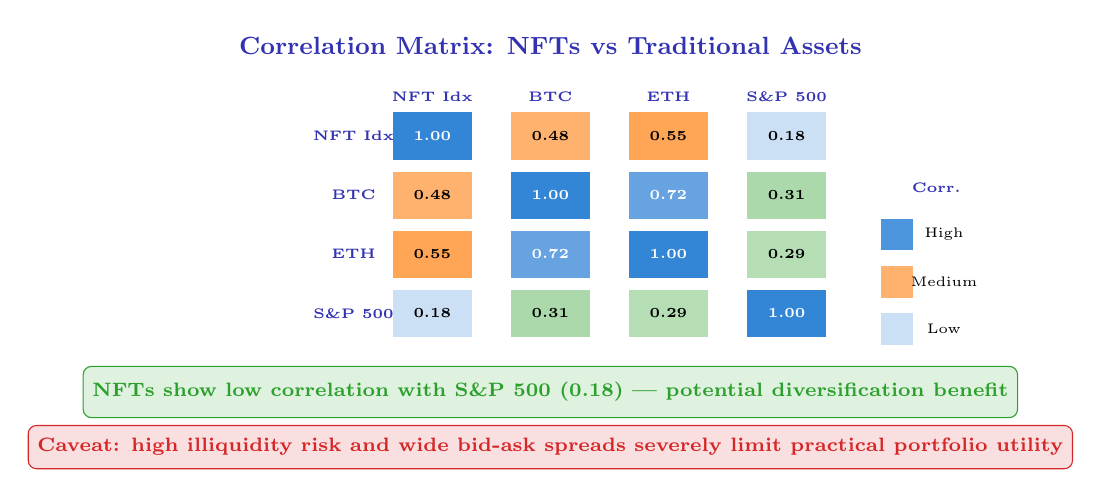
\begin{tikzpicture}[remember picture]
  \node[font=\small\bfseries, text=mlpurple] at (6.0,5.6) {Correlation Matrix: NFTs vs Traditional Assets};

  % Correlation matrix (heatmap style) - 4x4
  % Assets: NFTs, BTC, ETH, SP500

  % Header row labels (columns)
  \node[font=\tiny\bfseries, text=mlpurple, align=center] at (4.5,4.95) {NFT Idx};
  \node[font=\tiny\bfseries, text=mlpurple, align=center] at (6.0,4.95) {BTC};
  \node[font=\tiny\bfseries, text=mlpurple, align=center] at (7.5,4.95) {ETH};
  \node[font=\tiny\bfseries, text=mlpurple, align=center] at (9.0,4.95) {S\&P 500};

  % Row 1: NFT Idx
  \node[font=\tiny\bfseries, text=mlpurple, align=right] at (3.5,4.45) {NFT Idx};
  \fill[mlblue!80] (4.0,4.15) rectangle (5.0,4.75);
  \node[font=\tiny\bfseries, text=white, align=center] at (4.5,4.45) {1.00};
  \fill[mlorange!60] (5.5,4.15) rectangle (6.5,4.75);
  \node[font=\tiny\bfseries, align=center] at (6.0,4.45) {0.48};
  \fill[mlorange!70] (7.0,4.15) rectangle (8.0,4.75);
  \node[font=\tiny\bfseries, align=center] at (7.5,4.45) {0.55};
  \fill[mlblue!20] (8.5,4.15) rectangle (9.5,4.75);
  \node[font=\tiny\bfseries, align=center] at (9.0,4.45) {0.18};

  % Row 2: BTC
  \node[font=\tiny\bfseries, text=mlpurple, align=right] at (3.5,3.7) {BTC};
  \fill[mlorange!60] (4.0,3.4) rectangle (5.0,4.0);
  \node[font=\tiny\bfseries, align=center] at (4.5,3.7) {0.48};
  \fill[mlblue!80] (5.5,3.4) rectangle (6.5,4.0);
  \node[font=\tiny\bfseries, text=white, align=center] at (6.0,3.7) {1.00};
  \fill[mlblue!60] (7.0,3.4) rectangle (8.0,4.0);
  \node[font=\tiny\bfseries, text=white, align=center] at (7.5,3.7) {0.72};
  \fill[mlgreen!40] (8.5,3.4) rectangle (9.5,4.0);
  \node[font=\tiny\bfseries, align=center] at (9.0,3.7) {0.31};

  % Row 3: ETH
  \node[font=\tiny\bfseries, text=mlpurple, align=right] at (3.5,2.95) {ETH};
  \fill[mlorange!70] (4.0,2.65) rectangle (5.0,3.25);
  \node[font=\tiny\bfseries, align=center] at (4.5,2.95) {0.55};
  \fill[mlblue!60] (5.5,2.65) rectangle (6.5,3.25);
  \node[font=\tiny\bfseries, text=white, align=center] at (6.0,2.95) {0.72};
  \fill[mlblue!80] (7.0,2.65) rectangle (8.0,3.25);
  \node[font=\tiny\bfseries, text=white, align=center] at (7.5,2.95) {1.00};
  \fill[mlgreen!35] (8.5,2.65) rectangle (9.5,3.25);
  \node[font=\tiny\bfseries, align=center] at (9.0,2.95) {0.29};

  % Row 4: SP500
  \node[font=\tiny\bfseries, text=mlpurple, align=right] at (3.5,2.2) {S\&P 500};
  \fill[mlblue!20] (4.0,1.9) rectangle (5.0,2.5);
  \node[font=\tiny\bfseries, align=center] at (4.5,2.2) {0.18};
  \fill[mlgreen!40] (5.5,1.9) rectangle (6.5,2.5);
  \node[font=\tiny\bfseries, align=center] at (6.0,2.2) {0.31};
  \fill[mlgreen!35] (7.0,1.9) rectangle (8.0,2.5);
  \node[font=\tiny\bfseries, align=center] at (7.5,2.2) {0.29};
  \fill[mlblue!80] (8.5,1.9) rectangle (9.5,2.5);
  \node[font=\tiny\bfseries, text=white, align=center] at (9.0,2.2) {1.00};

  % Color legend
  \fill[mlblue!20] (10.2,1.8) rectangle (10.6,2.2);
  \fill[mlorange!60] (10.2,2.4) rectangle (10.6,2.8);
  \fill[mlblue!70] (10.2,3.0) rectangle (10.6,3.4);
  \node[font=\tiny, align=left] at (11.0,2.0) {Low};
  \node[font=\tiny, align=left] at (11.0,2.6) {Medium};
  \node[font=\tiny, align=left] at (11.0,3.2) {High};
  \node[font=\tiny\bfseries, text=mlpurple, align=center] at (10.9,3.8) {Corr.};

  % Diversification note
  \node[draw=mlgreen, fill=mlgreen!15, rounded corners=3pt, minimum width=11.6cm, minimum height=0.65cm, font=\scriptsize\bfseries, align=center, text=mlgreen] at (6.0,1.2) {NFTs show low correlation with S\&P 500 (0.18) --- potential diversification benefit};
  \node[draw=mlred, fill=mlred!15, rounded corners=3pt, minimum width=11.6cm, minimum height=0.55cm, font=\scriptsize\bfseries, align=center, text=mlred] at (6.0,0.5) {Caveat: high illiquidity risk and wide bid-ask spreads severely limit practical portfolio utility};
\end{tikzpicture}
\bottomnote{NFTs show low correlation with traditional assets but high illiquidity risk limits portfolio utility}
\end{frame}

% Frame 48: Section 4 Summary
\begin{frame}{Section 4 Summary}
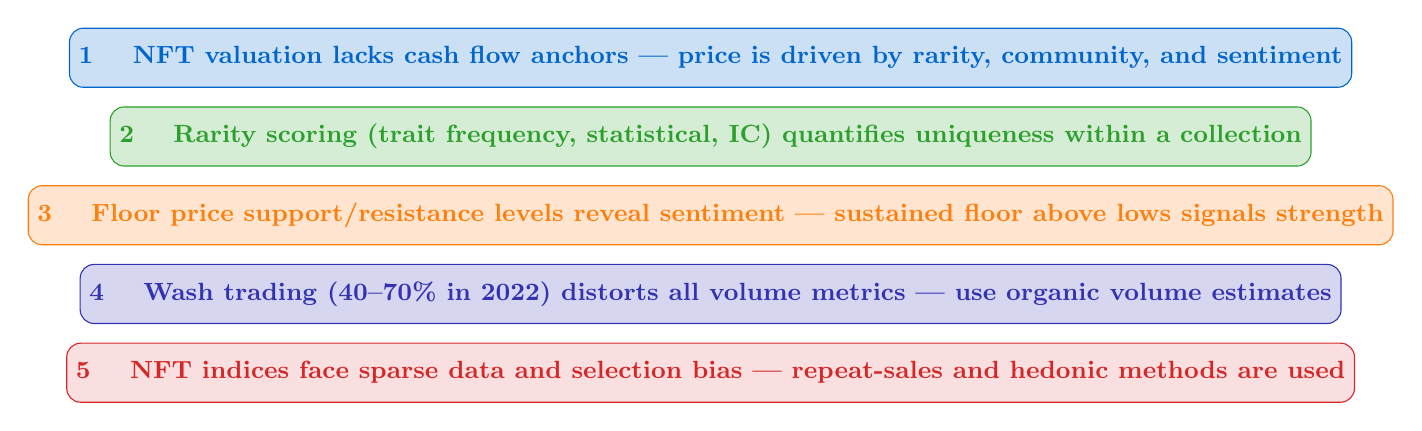
\begin{tikzpicture}[remember picture]
  \node[draw=mlblue, fill=mlblue!20, rounded corners=5pt, minimum width=11.6cm, minimum height=0.75cm, font=\small\bfseries, align=center, text=mlblue] at (6.0,5.2) {1 \quad NFT valuation lacks cash flow anchors --- price is driven by rarity, community, and sentiment};
  \node[draw=mlgreen, fill=mlgreen!20, rounded corners=5pt, minimum width=11.6cm, minimum height=0.75cm, font=\small\bfseries, align=center, text=mlgreen] at (6.0,4.2) {2 \quad Rarity scoring (trait frequency, statistical, IC) quantifies uniqueness within a collection};
  \node[draw=mlorange, fill=mlorange!20, rounded corners=5pt, minimum width=11.6cm, minimum height=0.75cm, font=\small\bfseries, align=center, text=mlorange] at (6.0,3.2) {3 \quad Floor price support/resistance levels reveal sentiment --- sustained floor above lows signals strength};
  \node[draw=mlpurple, fill=mlpurple!20, rounded corners=5pt, minimum width=11.6cm, minimum height=0.75cm, font=\small\bfseries, align=center, text=mlpurple] at (6.0,2.2) {4 \quad Wash trading (40--70\% in 2022) distorts all volume metrics --- use organic volume estimates};
  \node[draw=mlred, fill=mlred!15, rounded corners=5pt, minimum width=11.6cm, minimum height=0.75cm, font=\small\bfseries, align=center, text=mlred] at (6.0,1.2) {5 \quad NFT indices face sparse data and selection bias --- repeat-sales and hedonic methods are used};
\end{tikzpicture}
\bottomnote{Section 4 complete -- next: Advanced Topics \& Future}
\end{frame}

%% ============================================================
%% SECTION 5: ADVANCED TOPICS & FUTURE
%% ============================================================
\section{Advanced Topics \& Future}

% Frame 49: Section 5 Divider
\begin{frame}{Section 5: Advanced Topics \& Future}
\begin{beamercolorbox}[sep=12pt,center,rounded=true,shadow=true]{palette quaternary}
  {\Large\bfseries Section 5: Advanced Topics \& Future}\\[4pt]
  {\normalsize Fractional NFTs, dynamic NFTs, soulbound tokens, composability, and regulation}
\end{beamercolorbox}

\vspace{4mm}
\begin{columns}[T]
\column{0.55\textwidth}
\begin{block}{What You Will Learn}
\begin{itemize}\setlength{\itemsep}{2pt}
  \item Fractional NFTs: splitting high-value assets via ERC-20 tokens
  \item Dynamic NFTs: metadata that changes in response to real-world events
  \item Soulbound tokens: non-transferable identity and reputation
  \item ERC-6551: token-bound accounts and NFT composability
  \item The evolving global regulatory landscape for NFTs
\end{itemize}
\end{block}
\column{0.42\textwidth}
\begin{block}{Frames in This Section}
\begin{itemize}\setlength{\itemsep}{1pt}
  \item Frame 49 --- Section overview
  \item Frame 50 --- Fractional NFTs
  \item Frame 51 --- Dynamic NFTs (dNFTs)
  \item Frame 52 --- Soulbound tokens
  \item Frame 53 --- NFT composability
  \item Frame 54 --- Regulatory landscape
  \item Frame 55 --- Key takeaways
\end{itemize}
\end{block}
\end{columns}
\bottomnote{Section 5 | Frames 49--55 | Advanced Topics \& Future}
\end{frame}

% Frame 50: Fractional NFTs [FRAGILE] -- CODE FRAME 3
\begin{frame}[fragile]{Fractional NFTs}
\begin{columns}[T]
\column{0.48\textwidth}
\begin{block}{What is Fractionalization?}
\begin{itemize}\setlength{\itemsep}{3pt}
  \item A high-value NFT (e.g.\ CryptoPunk \$10M) is locked in a \textbf{vault contract}
  \item The vault mints a fixed supply of \textbf{ERC-20 tokens} representing fractional ownership
  \item Fractions are tradeable on any DEX --- lowering entry barrier
  \item Governance vote required to unlock and sell the underlying NFT
  \item Examples: Fractional.art (now Tessera), NFTX, PartyDAO
\end{itemize}
\end{block}
\vspace{2mm}
\begin{block}{Economic Benefit}
Fractionalization enables price discovery and liquidity for illiquid, high-value NFTs --- analogous to REITs for real estate.
\end{block}

\column{0.49\textwidth}
\begin{lstlisting}[language=Solidity]
// Simplified NFT Fractionalization
contract FractionalVault {
    IERC721 public nft;
    uint256 public tokenId;
    ERC20 public fractions;

    function fractionalize(
        address _nft, uint256 _id,
        uint256 totalFractions
    ) external {
        IERC721(_nft).transferFrom(
            msg.sender, address(this), _id
        );
        fractions.mint(
            msg.sender, totalFractions
        );
    }
}
\end{lstlisting}
\end{columns}
\bottomnote{Fractional NFTs lower the barrier to entry by splitting ownership into ERC-20 tokens}
\end{frame}

% Frame 51: Dynamic NFTs (dNFTs)
\begin{frame}{Dynamic NFTs (dNFTs)}
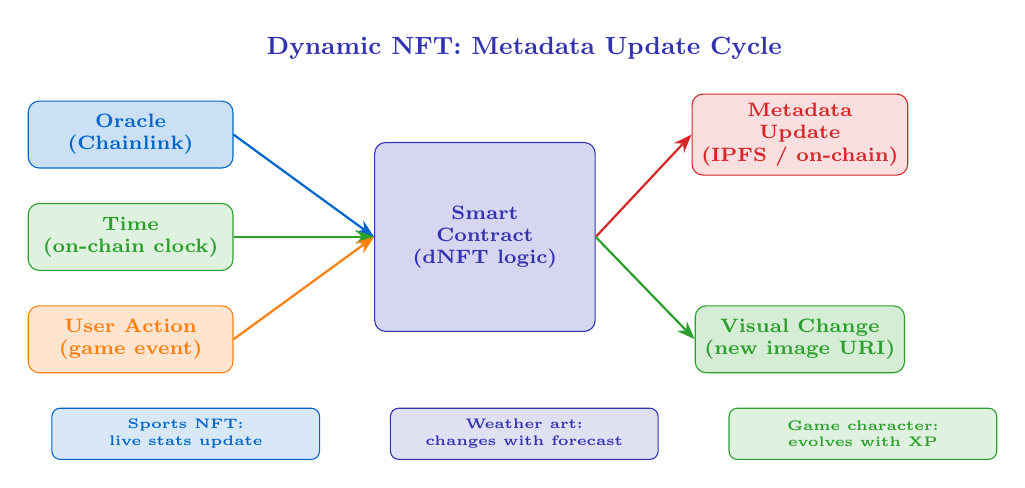
\begin{tikzpicture}[remember picture]
  \node[font=\small\bfseries, text=mlpurple] at (6.0,5.6) {Dynamic NFT: Metadata Update Cycle};

  % Trigger sources
  \node[draw=mlblue, fill=mlblue!20, rounded corners=4pt, minimum width=2.6cm, minimum height=0.85cm, font=\scriptsize\bfseries, align=center, text=mlblue] (oracle) at (1.0,4.5) {Oracle\\(Chainlink)};
  \node[draw=mlgreen, fill=mlgreen!15, rounded corners=4pt, minimum width=2.6cm, minimum height=0.85cm, font=\scriptsize\bfseries, align=center, text=mlgreen] (time) at (1.0,3.2) {Time\\(on-chain clock)};
  \node[draw=mlorange, fill=mlorange!20, rounded corners=4pt, minimum width=2.6cm, minimum height=0.85cm, font=\scriptsize\bfseries, align=center, text=mlorange] (useract) at (1.0,1.9) {User Action\\(game event)};

  % Smart contract
  \node[draw=mlpurple, fill=mlpurple!20, rounded corners=4pt, minimum width=2.8cm, minimum height=2.4cm, font=\scriptsize\bfseries, align=center, text=mlpurple] (sc) at (5.5,3.2) {Smart\\Contract\\(dNFT logic)};

  % Metadata update
  \node[draw=mlred, fill=mlred!15, rounded corners=4pt, minimum width=2.6cm, minimum height=0.85cm, font=\scriptsize\bfseries, align=center, text=mlred] (meta) at (9.5,4.5) {Metadata\\Update\\(IPFS / on-chain)};

  % Visual change
  \node[draw=mlgreen, fill=mlgreen!20, rounded corners=4pt, minimum width=2.6cm, minimum height=0.85cm, font=\scriptsize\bfseries, align=center, text=mlgreen] (visual) at (9.5,1.9) {Visual Change\\(new image URI)};

  % Arrows
  \draw[-{Stealth}, thick, mlblue] (oracle.east) -- (sc.west);
  \draw[-{Stealth}, thick, mlgreen] (time.east) -- (sc.west);
  \draw[-{Stealth}, thick, mlorange] (useract.east) -- (sc.west);
  \draw[-{Stealth}, thick, mlred] (sc.east) -- (meta.west);
  \draw[-{Stealth}, thick, mlgreen] (sc.east) -- (visual.west);

  % Examples
  \node[draw=mlblue, fill=mlblue!15, rounded corners=3pt, minimum width=3.4cm, minimum height=0.65cm, font=\tiny\bfseries, align=center, text=mlblue] at (1.7,0.7) {Sports NFT:\\live stats update};
  \node[draw=mlpurple, fill=mlpurple!15, rounded corners=3pt, minimum width=3.4cm, minimum height=0.65cm, font=\tiny\bfseries, align=center, text=mlpurple] at (6.0,0.7) {Weather art:\\changes with forecast};
  \node[draw=mlgreen, fill=mlgreen!15, rounded corners=3pt, minimum width=3.4cm, minimum height=0.65cm, font=\tiny\bfseries, align=center, text=mlgreen] at (10.3,0.7) {Game character:\\evolves with XP};
\end{tikzpicture}
\bottomnote{Dynamic NFTs can change their metadata based on external data}
\end{frame}

% Frame 52: Soulbound Tokens (SBTs)
\begin{frame}{Soulbound Tokens (SBTs)}
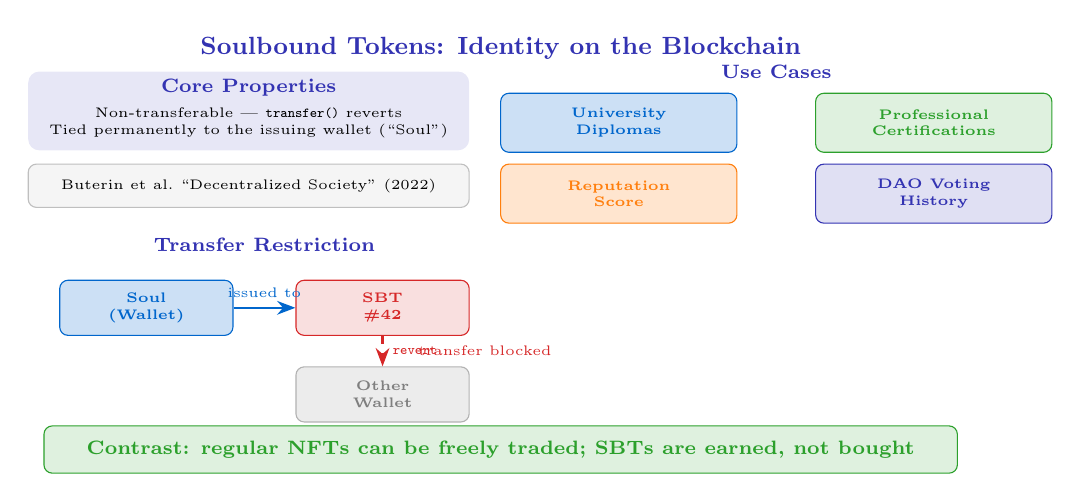
\begin{tikzpicture}[remember picture]
  \node[font=\small\bfseries, text=mlpurple] at (6.0,5.6) {Soulbound Tokens: Identity on the Blockchain};

  % Core properties panel
  \fill[mlpurple!12, rounded corners=4pt] (0,4.3) rectangle (5.6,5.3);
  \node[font=\scriptsize\bfseries, text=mlpurple] at (2.8,5.1) {Core Properties};
  \node[font=\tiny, align=center] at (2.8,4.65) {Non-transferable --- \texttt{transfer()} reverts\\Tied permanently to the issuing wallet (``Soul'')};

  % Buterin reference
  \node[draw=mlgray!50, fill=mlgray!8, rounded corners=3pt, minimum width=5.6cm, minimum height=0.55cm, font=\tiny, align=center] at (2.8,3.85) {Buterin et al.\ ``Decentralized Society'' (2022)};

  % Use case grid
  \node[font=\scriptsize\bfseries, text=mlpurple] at (9.5,5.3) {Use Cases};

  \node[draw=mlblue, fill=mlblue!20, rounded corners=3pt, minimum width=3.0cm, minimum height=0.75cm, font=\tiny\bfseries, align=center, text=mlblue] at (7.5,4.65) {University\\Diplomas};
  \node[draw=mlgreen, fill=mlgreen!15, rounded corners=3pt, minimum width=3.0cm, minimum height=0.75cm, font=\tiny\bfseries, align=center, text=mlgreen] at (11.5,4.65) {Professional\\Certifications};
  \node[draw=mlorange, fill=mlorange!20, rounded corners=3pt, minimum width=3.0cm, minimum height=0.75cm, font=\tiny\bfseries, align=center, text=mlorange] at (7.5,3.75) {Reputation\\Score};
  \node[draw=mlpurple, fill=mlpurple!15, rounded corners=3pt, minimum width=3.0cm, minimum height=0.75cm, font=\tiny\bfseries, align=center, text=mlpurple] at (11.5,3.75) {DAO Voting\\History};

  % Transfer restriction diagram
  \node[font=\scriptsize\bfseries, text=mlpurple] at (3.0,3.1) {Transfer Restriction};

  \node[draw=mlblue, fill=mlblue!20, rounded corners=3pt, minimum width=2.2cm, minimum height=0.7cm, font=\tiny\bfseries, align=center, text=mlblue] (soul) at (1.5,2.3) {Soul\\(Wallet)};
  \node[draw=mlred, fill=mlred!15, rounded corners=3pt, minimum width=2.2cm, minimum height=0.7cm, font=\tiny\bfseries, align=center, text=mlred] (sbt) at (4.5,2.3) {SBT\\\#42};
  \node[draw=mlgray!60, fill=mlgray!15, rounded corners=3pt, minimum width=2.2cm, minimum height=0.7cm, font=\tiny\bfseries, align=center, text=mlgray] (other) at (4.5,1.2) {Other\\Wallet};

  \draw[-{Stealth}, thick, mlblue] (soul.east) -- node[above, font=\tiny] {issued to} (sbt.west);
  \draw[-{Stealth}, thick, mlred, dashed] (sbt.south) -- node[right, font=\tiny, text=mlred] {\texttt{revert}} (other.north);
  \node[font=\tiny, text=mlred] at (5.8,1.75) {transfer blocked};

  % Contrast with transferable
  \node[draw=mlgreen, fill=mlgreen!15, rounded corners=3pt, minimum width=11.6cm, minimum height=0.6cm, font=\scriptsize\bfseries, align=center, text=mlgreen] at (6.0,0.5) {Contrast: regular NFTs can be freely traded; SBTs are earned, not bought};
\end{tikzpicture}
\bottomnote{Soulbound tokens represent identity and reputation -- they cannot be bought or sold, only earned}
\end{frame}

% Frame 53: NFT Composability and Nesting (ERC-6551)
\begin{frame}{NFT Composability and Nesting}
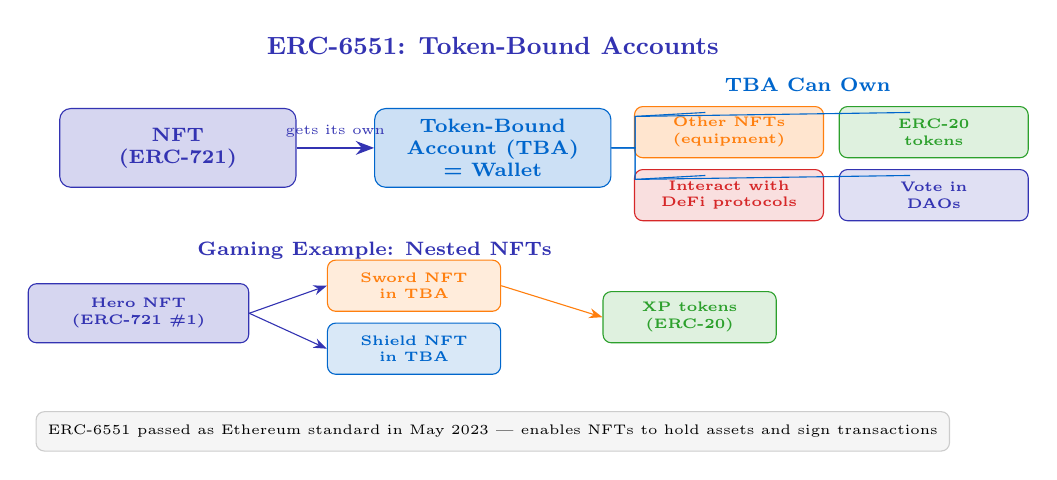
\begin{tikzpicture}[remember picture]
  \node[font=\small\bfseries, text=mlpurple] at (6.0,5.6) {ERC-6551: Token-Bound Accounts};

  % ERC-6551 concept
  \node[draw=mlpurple, fill=mlpurple!20, rounded corners=4pt, minimum width=3.0cm, minimum height=1.0cm, font=\scriptsize\bfseries, align=center, text=mlpurple] (nft) at (2.0,4.3) {NFT\\(ERC-721)};
  \node[draw=mlblue, fill=mlblue!20, rounded corners=4pt, minimum width=3.0cm, minimum height=1.0cm, font=\scriptsize\bfseries, align=center, text=mlblue] (tba) at (6.0,4.3) {Token-Bound\\Account (TBA)\\= Wallet};
  \draw[-{Stealth}, thick, mlpurple] (nft.east) -- node[above, font=\tiny] {gets its own} (tba.west);

  % What TBA can own
  \node[font=\scriptsize\bfseries, text=mlblue] at (10.0,5.1) {TBA Can Own};
  \node[draw=mlorange, fill=mlorange!20, rounded corners=3pt, minimum width=2.4cm, minimum height=0.65cm, font=\tiny\bfseries, align=center, text=mlorange] at (9.0,4.5) {Other NFTs\\(equipment)};
  \node[draw=mlgreen, fill=mlgreen!15, rounded corners=3pt, minimum width=2.4cm, minimum height=0.65cm, font=\tiny\bfseries, align=center, text=mlgreen] at (11.6,4.5) {ERC-20\\tokens};
  \node[draw=mlred, fill=mlred!15, rounded corners=3pt, minimum width=2.4cm, minimum height=0.65cm, font=\tiny\bfseries, align=center, text=mlred] at (9.0,3.7) {Interact with\\DeFi protocols};
  \node[draw=mlpurple, fill=mlpurple!15, rounded corners=3pt, minimum width=2.4cm, minimum height=0.65cm, font=\tiny\bfseries, align=center, text=mlpurple] at (11.6,3.7) {Vote in\\DAOs};

  \draw[thin, mlblue] (tba.east) -- ++(0.3,0) -- ++(0,0.4) -- (8.7,4.75);
  \draw[thin, mlblue] (tba.east) -- ++(0.3,0) -- ++(0,0.4) -- (11.3,4.75);
  \draw[thin, mlblue] (tba.east) -- ++(0.3,0) -- ++(0,-0.4) -- (8.7,3.95);
  \draw[thin, mlblue] (tba.east) -- ++(0.3,0) -- ++(0,-0.4) -- (11.3,3.95);

  % Game example
  \node[font=\scriptsize\bfseries, text=mlpurple] at (4.5,3.0) {Gaming Example: Nested NFTs};

  \node[draw=mlpurple, fill=mlpurple!20, rounded corners=3pt, minimum width=2.8cm, minimum height=0.75cm, font=\tiny\bfseries, align=center, text=mlpurple] (hero) at (1.5,2.2) {Hero NFT\\(ERC-721 \#1)};
  \node[draw=mlorange, fill=mlorange!15, rounded corners=3pt, minimum width=2.2cm, minimum height=0.65cm, font=\tiny\bfseries, align=center, text=mlorange] (sword) at (5.0,2.55) {Sword NFT\\in TBA};
  \node[draw=mlblue, fill=mlblue!15, rounded corners=3pt, minimum width=2.2cm, minimum height=0.65cm, font=\tiny\bfseries, align=center, text=mlblue] (shield) at (5.0,1.75) {Shield NFT\\in TBA};
  \node[draw=mlgreen, fill=mlgreen!15, rounded corners=3pt, minimum width=2.2cm, minimum height=0.65cm, font=\tiny\bfseries, align=center, text=mlgreen] (xp) at (8.5,2.15) {XP tokens\\(ERC-20)};

  \draw[-{Stealth}, thin, mlpurple] (hero.east) -- (sword.west);
  \draw[-{Stealth}, thin, mlpurple] (hero.east) -- (shield.west);
  \draw[-{Stealth}, thin, mlorange] (sword.east) -- (xp.west);

  \node[draw=mlgray!40, fill=mlgray!8, rounded corners=3pt, minimum width=11.6cm, minimum height=0.5cm, font=\tiny, align=center] at (6.0,0.7) {ERC-6551 passed as Ethereum standard in May 2023 --- enables NFTs to hold assets and sign transactions};
\end{tikzpicture}
\bottomnote{ERC-6551 gives every NFT its own wallet, enabling NFTs to own assets and interact with protocols}
\end{frame}

% Frame 54: NFT Regulation Landscape
\begin{frame}{NFT Regulation Landscape}
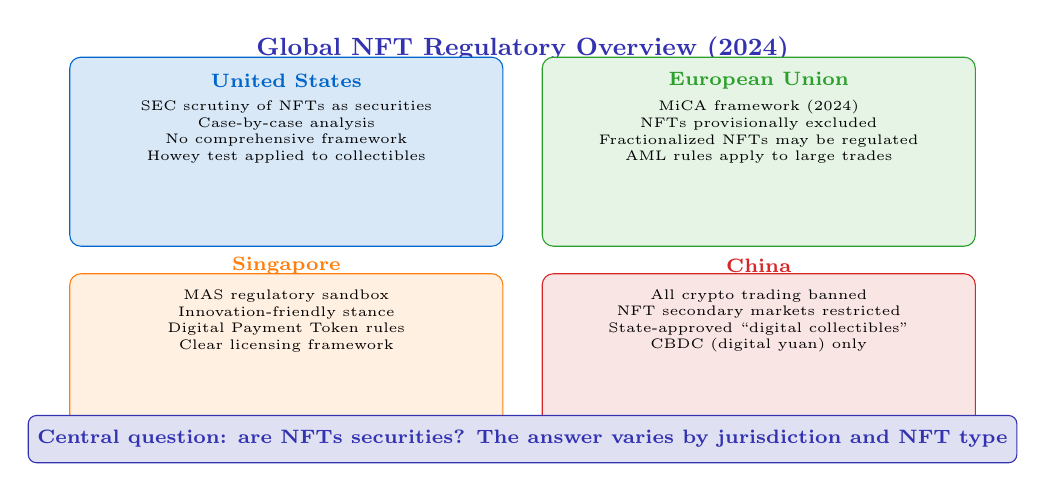
\begin{tikzpicture}[remember picture]
  \node[font=\small\bfseries, text=mlpurple] at (6.0,5.6) {Global NFT Regulatory Overview (2024)};

  % US box
  \node[draw=mlblue, fill=mlblue!15, rounded corners=4pt, minimum width=5.5cm, minimum height=2.4cm, font=\scriptsize\bfseries, align=center, text=mlblue] (us) at (3.0,4.3) {};
  \node[font=\scriptsize\bfseries, text=mlblue, align=center] at (3.0,5.2) {United States};
  \node[font=\tiny, align=center] at (3.0,4.55) {SEC scrutiny of NFTs as securities\\Case-by-case analysis\\No comprehensive framework\\Howey test applied to collectibles};

  % EU box
  \node[draw=mlgreen, fill=mlgreen!12, rounded corners=4pt, minimum width=5.5cm, minimum height=2.4cm, font=\scriptsize\bfseries, align=center, text=mlgreen] (eu) at (9.0,4.3) {};
  \node[font=\scriptsize\bfseries, text=mlgreen, align=center] at (9.0,5.2) {European Union};
  \node[font=\tiny, align=center] at (9.0,4.55) {MiCA framework (2024)\\NFTs provisionally excluded\\Fractionalized NFTs may be regulated\\AML rules apply to large trades};

  % Singapore box
  \node[draw=mlorange, fill=mlorange!12, rounded corners=4pt, minimum width=5.5cm, minimum height=2.0cm, font=\scriptsize\bfseries, align=center, text=mlorange] (sg) at (3.0,1.75) {};
  \node[font=\scriptsize\bfseries, text=mlorange, align=center] at (3.0,2.85) {Singapore};
  \node[font=\tiny, align=center] at (3.0,2.15) {MAS regulatory sandbox\\Innovation-friendly stance\\Digital Payment Token rules\\Clear licensing framework};

  % China box
  \node[draw=mlred, fill=mlred!12, rounded corners=4pt, minimum width=5.5cm, minimum height=2.0cm, font=\scriptsize\bfseries, align=center, text=mlred] (cn) at (9.0,1.75) {};
  \node[font=\scriptsize\bfseries, text=mlred, align=center] at (9.0,2.85) {China};
  \node[font=\tiny, align=center] at (9.0,2.15) {All crypto trading banned\\NFT secondary markets restricted\\State-approved ``digital collectibles''\\CBDC (digital yuan) only};

  % Key question box
  \node[draw=mlpurple, fill=mlpurple!15, rounded corners=3pt, minimum width=11.6cm, minimum height=0.6cm, font=\scriptsize\bfseries, align=center, text=mlpurple] at (6.0,0.65) {Central question: are NFTs securities? The answer varies by jurisdiction and NFT type};
\end{tikzpicture}
\bottomnote{NFT regulation is evolving rapidly -- the classification of NFTs as securities remains a central debate}
\end{frame}

% Frame 55: Key Takeaways and Course Summary
\begin{frame}{Key Takeaways and Course Summary}
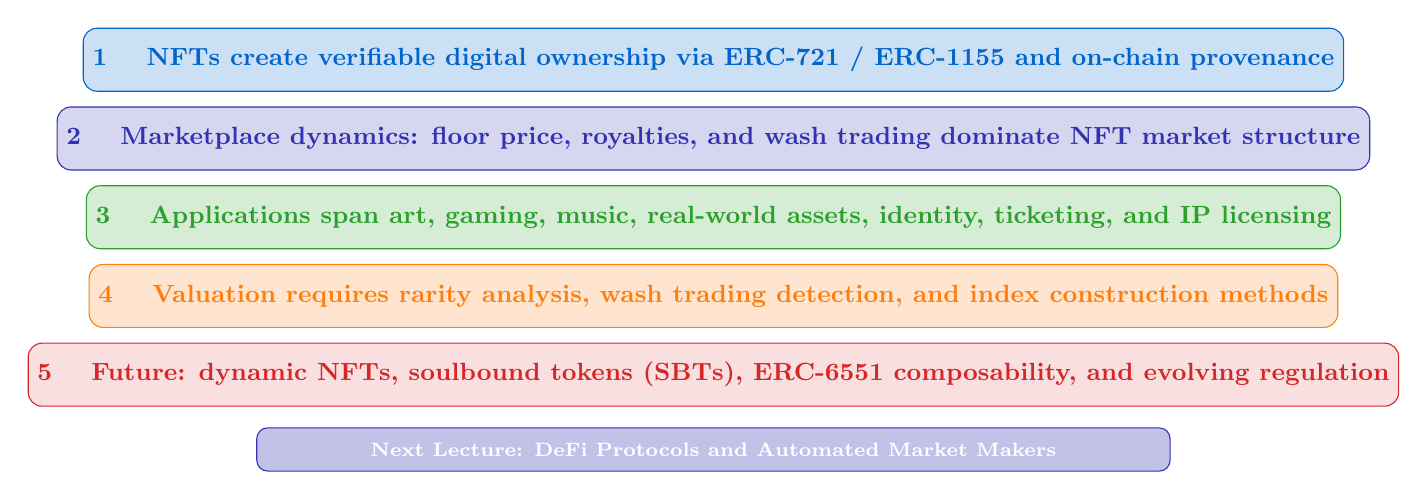
\begin{tikzpicture}[remember picture]
  \node[draw=mlblue, fill=mlblue!20, rounded corners=5pt, minimum width=11.6cm, minimum height=0.8cm, font=\small\bfseries, align=center, text=mlblue] at (6.0,5.25) {1 \quad NFTs create verifiable digital ownership via ERC-721 / ERC-1155 and on-chain provenance};
  \node[draw=mlpurple, fill=mlpurple!20, rounded corners=5pt, minimum width=11.6cm, minimum height=0.8cm, font=\small\bfseries, align=center, text=mlpurple] at (6.0,4.25) {2 \quad Marketplace dynamics: floor price, royalties, and wash trading dominate NFT market structure};
  \node[draw=mlgreen, fill=mlgreen!20, rounded corners=5pt, minimum width=11.6cm, minimum height=0.8cm, font=\small\bfseries, align=center, text=mlgreen] at (6.0,3.25) {3 \quad Applications span art, gaming, music, real-world assets, identity, ticketing, and IP licensing};
  \node[draw=mlorange, fill=mlorange!20, rounded corners=5pt, minimum width=11.6cm, minimum height=0.8cm, font=\small\bfseries, align=center, text=mlorange] at (6.0,2.25) {4 \quad Valuation requires rarity analysis, wash trading detection, and index construction methods};
  \node[draw=mlred, fill=mlred!15, rounded corners=5pt, minimum width=11.6cm, minimum height=0.8cm, font=\small\bfseries, align=center, text=mlred] at (6.0,1.25) {5 \quad Future: dynamic NFTs, soulbound tokens (SBTs), ERC-6551 composability, and evolving regulation};

  \node[draw=mlpurple, fill=mlpurple!30, rounded corners=4pt, minimum width=11.6cm, minimum height=0.55cm, font=\scriptsize\bfseries, align=center, text=white] at (6.0,0.3) {Next Lecture: DeFi Protocols and Automated Market Makers};
\end{tikzpicture}
\bottomnote{End of lecture -- 55 frames covering NFT fundamentals to advanced topics.}
\end{frame}

\end{document}
